\documentclass[openright]{normas-utf-tex} %openright = o capitulo comeca sempre em paginas impares

\special{papersize=210mm,297mm}

\usepackage[alf,abnt-emphasize=bf,bibjustif,recuo=0cm, abnt-etal-cite=2, abnt-etal-list=99]{abntcite} %configuracao correta das referencias bibliograficas.

\usepackage[brazil]{babel} % pacote portugues brasileiro
\usepackage[utf8]{inputenc} % pacote para acentuacao direta
\usepackage{amsmath,amsfonts,amssymb} % pacote matematico
\usepackage{graphicx} % pacote grafico
\usepackage{times} % fonte times
\usepackage[final]{pdfpages} % adicao da ata
\usepackage{float}
\usepackage{scalefnt}
\usepackage{algorithmic}% http://ctan.org/pkg/algorithms

\instituicao{Universidade Tecnológica Federal do Paraná} % nome da instituicao
\programa{Programa de Pós-graduação em Engenharia Elétrica e Informática Industrial} % nome do programa
\area{Informática Industrial} % [Engenharia Biom\'edica] ou [Inform\'atica Industrial] ou [Telem\'atica]

\documento{Dissertação} % [Disserta\c{c}\~ao] ou [Tese]
\nivel{Mestrado} % [Mestrado] ou [Doutorado]
\titulacao{Mestre} % [Mestre] ou [Doutor]

\titulo{{Proposta de um modelo para representar cenários de acidente usando conceitos de Norma, Sanção e Violação}} % titulo do trabalho em portugues
\title{\MakeUppercase{Title in English}} % titulo do trabalho em ingles

\autor{Jonathan Morris Samara} % autor do trabalho
\cita{Morris Samara, Jonathan} % sobrenome (maiusculas), nome do autor do trabalho

\palavraschave{sistema multiagente, norma, sanção, violação} % palavras-chave do trabalho
\keywords{Keyword 1, Keyword 2, ...} % palavras-chave do trabalho em ingles

\comentario{\UTFPRdocumentodata\ apresentada ao \UTFPRprogramadata\ da \ABNTinstituicaodata\ como requisito parcial para obtenção do grau de ``\UTFPRtitulacaodata\ em Ciências'' -- Área de Concentração: \UTFPRareadata.}

\orientador{Cesar Augusto Tacla} 
\local{Curitiba} % cidade
\data{\the\year} % ano automatico

% desativa hifenizacao mantendo o texto justificado.
% thanks to Emilio C. G. Wille
\tolerance=1
\emergencystretch=\maxdimen
\hyphenpenalty=10000
\hbadness=10000
\sloppy

%---------- Inicio do Documento ----------
\begin{document}

\capa % geracao automatica da capa
\folhaderosto % geracao automatica da folha de rosto

% Lembre-se de que a ficha catalografica eh impressa no verso da folha de rosto
% Ficha catalografica
\fichacatpum{T137}
\fichacatautor{Morris Samara, Jonathan}
\fichacatpgbib{\pageref{bibstart}-\pageref{bibend}}
\fichacatpalcha{1. Sistema Multiagente. 2. Normas. 3. Sanção, Violação}
\fichacatpdois{CDD (22. ed.) 621.3}
\fichacatbib{Biblioteca xxxxxx}
\fichacat

% insercao da ATA
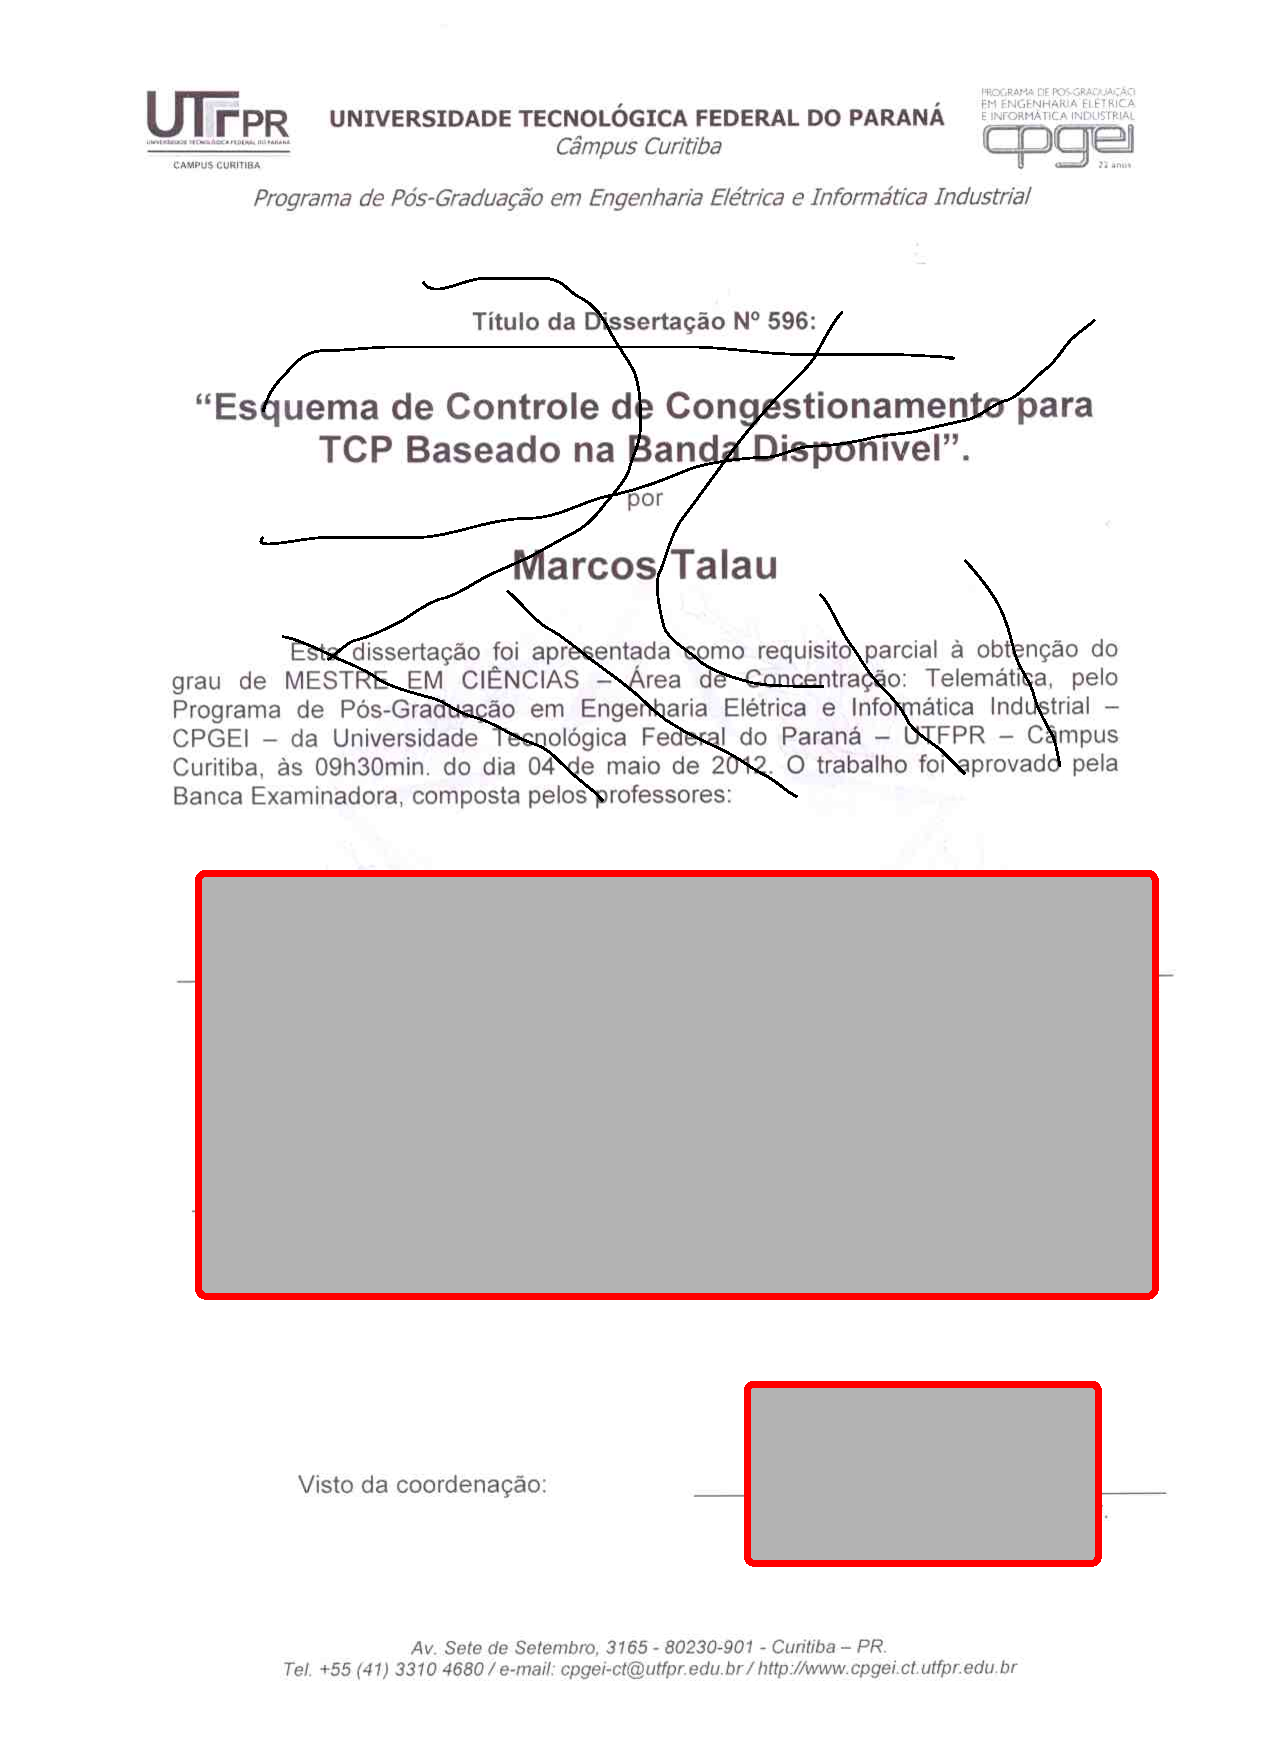
\includepdf{ata.pdf}

% dedicatoria
\begin{dedicatoria}
Texto da dedicat\'oria.
\end{dedicatoria}

% agradecimentos (opcional)
\begin{agradecimentos}
Texto dos agradecimentos.
\end{agradecimentos}

% epigrafe (opcional)
\begin{epigrafe}
Texto da ep\'igrafe.
\end{epigrafe}

%resumo
\begin{resumo}
Texto do resumo (m\'aximo de 500 palavras).
\end{resumo}

%abstract
\begin{abstract}
Abstract text (maximum of 500 words).
\end{abstract}

% listas (opcionais, mas recomenda-se a partir de 5 elementos)
\listadefiguras % geracao automatica da lista de figuras
\listadetabelas % geracao automatica da lista de tabelas
\listadequadros % adivinhe :)
\listadesiglas % geracao automatica da lista de siglas
\listadesimbolos % geracao automatica da lista de simbolos

% sumario
\sumario % geracao automatica do sumario

\setcounter{page}{12}

%---------- Primeiro Capitulo ----------
\chapter{Introdução}

	Diversas pessoas são submetidas a algum tipo de risco na execução de atividades profissionais. Trabalhos como de eletricistas, bombeiros, área petroquímica, serviços de telecomunicações e de transporte (motoristas de ônibus e de carro) são apenas alguns em que onde profissionais são expostos a condições de risco.

Acidentes em situações assim ocorrem pelos mais diversos motivos. Investigar as cadeias de causalidade que resultam nessas situações pode trazer um entendimento de como lidar com essas circunstâncias. Consequentemente, isso traz um potencial para diminuir o número de acidentes. A computação é uma ciência que apresenta um grande potencial de contribuição para a resolução desse problema. Isso envolve criar representações que descrevam atividades com riscos de acidentes e que permitam realizar raciocínios sobre essas relações de causalidade.

Algo que exemplifica essa situação são as atividades praticadas por profissionais que trabalham com eletricidade em linha viva. Isso, pois esses trabalhadores realizam procedimentos de manutenção em componentes, estruturas e equipamentos elétricos energizados que demandam fluxo de potência elétrica (ex. transformadores, condutores). A particularidade nos processos de linha viva consiste no fato de que esses equipamentos e estruturas se mantêm energizados durante a ação dos profissionais. Essa situação expõem esses profissionais a perigos de acidentes com eletricidade causando mortes ou ferimentos extremamente sérios com danos permanentes a vida dos acidentados.  
	
	\section{Motivação}	
		\label{motivation}
		Uma das motivações desse estudo reside em obter uma compreensão do problema em voga por meio de um modelo conceitual concebido com base em dois fatores. O primeiro fator consiste numa averiguação de modelos computacionais que são aplicados em sistemas multiagentes (inclusive os normativos). O segundo fator consiste em averiguar um dado estudo de caso a fim de abstrair estruturas conceituais que possam ser do interesse dessa pesquisa.

Uma outra motivação desse estudo consiste em averiguar como o modelo conceitual resultante pode ser vinculado a arcabouços e modelos computacionais que fazem parte do \textit{mainframe} acadêmico no campo da computação em sistemas multiagentes normativos.

A motivação desse estudo, portanto, reside em explorar e entender a problemática atrelada a cenários de acidentes e riscos com a finalidade de avaliar com clareza as possibilidades existentes dentro do contexto computacional.
	
	\section{Relevância}
		\label{relevance}
		A computação pode contribuir de inúmeras maneiras por conceber sistemas que resolvam de diferentes formas os problemas atrelados a acidentes de manutenção. Contudo, isso não pode ser feito sem um entendimento, em termos conceituais e computacionais, do estado deste problema. Por conta disso, os autores entendem que a relevância desse estudo reside na apresentação de um modelo conceitual que defina em termos de classes e relacionamento uma estrutura lógico-descritiva de fatores ambientais e organizacionais que resultam em acidentes. 

Por mais que existam modelos computacionais altamente sofisticados que possam ser aplicados a situações assim, um modelo conceitual dessa problemática apresenta potencial de análise de novas perspectivas do problema. Assim sendo, esse estudo também é relevante por estimular o debate do uso da computação em cenários de acidentes explorando novos tópicos de reflexão. Sendo que esse estudo visa explorar esse problema a partir de uma análise criativa, contudo racional, lógica, transparente e científica. 

	\section{Objetivos}
		\label{goals}
		Essa subseção tem a finalidade de apresentar o objetivo geral bem como os objetivos específicos dessa pesquisa. 

		\subsection{Objetivo Geral}

			Sintetizar, construir e avaliar, por intermédio de observações, de análises de documentos técnicos, de análises de modelos computacionais e de entrevista com profissionais da área, um modelo conceitual que define os conceitos e as relações para representar os cenários de ambientes de atividades, bem como os respectivos acidentes que podem acontecer, em que a validação ocorre por verificar se os raciocínios (para um dado estudo de caso do setor de energia elétrica) resultantes desse modelo são correspondentes com a realidade a fim de levantar um entendimento formal do problema para a comunidade acadêmica no que tange a que tipo de representação computacional é mais apropriada para determinado contexto. 
			
		\subsection{Objetivos Específicos}

			\begin{itemize}
    \item Identificar os pontos essenciais que devem fazer parte da estrutura do modelo em relação aos riscos e consequências (acidentes) para os atores e atividades (continuidade), que sejam relevantes na prática da atividade de manutenção, em caso de falha na operação. 
    \item Construir um modelo conceitual que implementável computacionalmente e que produza as inferências que respondam às questões definidas como essenciais.
    \item Validar o modelo por aplica-lo a um dado estudo de caso a fim de averiguar se os raciocínios produzidos nessa situação estão de acordo com a realidade.  
    \item Analisar modelos computacionais em relação ao modelo conceitual desse estudo a fim de ter um levantamento formal do estado do problema.
\end{itemize}


%---------- Segundo Capitulo ----------

\chapter{Fundamentação Teórica}
\label{chap:fundteoric}

	Este capítulo apresenta os estudos que fundamentam essa pesquisa. Isso consiste em estudos acadêmicos que dão base para consolidação do modelo aqui proposto abrangendo seguintes áreas: Agentes, Artefatos, Sistemas Multiagentes, Normas (em conjunto com Violações e Sanções), Riscos e Lógica Modal. 

A palavra \textit{arcabouço} será usada em diversos momentos ao longo deste texto. O sentido desse termo deve ser interpretado como correspondente ao sentido do termo em inglês \textit{framework}.

	\section{Agentes} \label{agent}
 
		Não existe uma definição universal para tratar o conceito de agente sendo que esse tópico se encontra em meio a debates e controvérsias. Contudo, existe um entendimento generalizado de que 
um comportamento \textit{autonomo} é o cerne de noção que se tem por agente \cite{whatisagent}.  Apesar disso, a construção de um modelo computacional não pode ser feito sem uma definição. Assim sendo, nesse texto um agente é
 um sistema computacional que está situado em um dado ambiente e que apresenta comportamento autonomo \cite{definitionagent} \cite{whatisagent}. Não apenas isso, mas um agente faz uso
 so seu comportamento autonomo com o propósito de atingir objetivos que a ele é designado \cite{definitionagent} \cite{whatisagent}.

Dentro do contexto presente na definição de agentes, um ambiente apresenta as seguintes propriedades \cite{artificialinteligencemodermapproach} \cite{whatisagent}; 
\begin{itemize}
    \item \textit{Acessibilidade vs Inacessibilidade}; Um ambiente acessível é aquele onde um agente consegue ter informações claras, precisas e atualizadas no que tange a característica do ambiente.
    \item \textit{Determinístico vs Não-Determinístico}; Um comportamento determinístico é aquele onde uma ação possui um efeito claro e garantido, sem incertezas sobre o estado que irá resultar.
    \item \textit{Episódico vs Não-Episódico}; Um ambiente tende a ser o mais episódico possível tanto quando o desempenho do agente estiver associado a um episódio discreto e específico no ambiente.
    \item \textit{Estático vs Dinâmico}; Um ambiente é estático se não houver outros processos em parapelo aos eventos associados ao agente.
    \item \textit{Discreto vs Contínuo}; Um ambiente é discreto se existe um número finito de ações e percepções. 
\end{itemize}

Outro aspecto a ser considerado em um agente implica o comportamento autonomo. Uma entidade que possui essa natureza tem a capacidade agir por sí mesmo. Essa entidade não precisa de nenhuma outra entidade externa 
(ex. ser humano) para realizar decisões \cite{whatisagent} \cite{definitionagent}.

Há uma série de exemplos que se enquadram dentro dessa deinição. Sistemas de controle se enquadram nesses exemplos. Um \textit{termostato} é um sistema de controle que está em um dado ambiente 
(como um quarto ou uma sala) \cite{whatisagent}, gera dois sinais de saída (um desses sinais indica que a temperatura está baixa demais (ou alta demais dependendo da aplicação) e o outro sinal
demonstra que a temperatura está no nível aceitável). O termostato tem o seu comportamento autonomo baseado em duas regras \cite{whatisagent}:

\begin{itemize}
    \item Se a temperatura estiver abaixo (ou acima) do nível de temperatura definido, então ligar o atuador.
    \item Se a temperatura estiver dentro do nível estabelecido, então desligar o atuador.
\end{itemize}

Outro exemplo de agentes consiste nos programas \textit{Daemons} em sistemas \textit{UNIX}. Esses algoritmos trabalham em segundo plano e monitoram um dado ambiente de \textit{software}. Com base
em certas regras, na ocorrência de um dado evento no ambiente, esses programas realizam uma dada atuação \cite{whatisagent}.   

Os exemplos presentes neste texto são apropriados dentro do conceito de agentes. Contudo, esses exemplos não ase equandram dentro da denição de agentes inteligentes \cite{whatisagent}. Uma entidade que se enquadra
dentro das caracterísiticas de um agente inteligente deve necessariamente respeitar a definição já apresenta e deve apresentar as seguintes propriedades; reatividade (capaz de perceber as mudanças
que ocorrem no ambiente e responder a delas de maneira apropriada no que condiz aos objetivos do agente), pro-atividade (apresenta comportamento orientado a objetivos sendo que o agente toma as decisões
a fim de satisfazer os objetivos em interesse) e habilidades sociais (capacidade de interagir com outros agentes (e possivelmente humanos) a fim de poder satisfazer os próprios objetivos) \cite{whatisagent} \cite{artificialinteligencemodermapproach}.

Os agentes podem ser definidos em categorias. Um desses são agentes puramente reativos. Esses agentes tomam decisões considerando apenas informações que estão no instante presente. Por consequência, 
o comportamento deles ocorre por respostas diretas ao ambiente \cite{whatisagent}. 

Outra categoria de agentes são aqueles que possuem estados. Essas entidades possum uma dada estrutura de dados internar que são considerados quando agente toma uma uma certa decisão \cite{whatisagent}.

Uma outra maneira de analisar os agentes se dá por meio das arquiteturas e modelos disponiveis para representar os agentes (tomada de decisão, estado interno). Para o propósito do estudo que está
sendo apresentando neste texto, é o suficiente considerar de forma sucinta quatros dessas arquiteturas. A primeira consiste nos agentes baseados em lógica onde os agentes realizam deduções lógicas
para tomar uma decisão \cite{logicagent}, a segunda arquitetura consiste nos agentes reativos que tomam decisões com base em um dado mapeamento de uma certa situação em uma dada ação \cite{reactiveagent}, a terceira arquitetura é \textit{BDI}
cuja decisão ocorrem da manipulação de estruturas de dados que representam crenças, desejos e intenções do agente \cite{bdi} e a quarta arquitetura consiste em uma estrutura em camadas onde a tomada de decisão
acontecem por intermédio de diversas camadas abstração a cerca do ambiente \cite{layeragent} \cite{whatisagent}.  

	\section{Artefatos} \label{artefact}

		A definição de um artefato pode ser feita por analisar, antes, o comportamento de um agente. De maneira genérica, existe duas formas que podem ser usadas para caracterizar o comportamento de um agente, e essas são \textit{goal-governed} e \textit{goal-oriented} \cite{relationwithagentprogram} \cite{programingagentartefact}.

Um agente que é caracterizado como \textit{goal-governed} são aqueles que apresentam capacidades cognitivas, que podem representar os seus respectivos objetivos e, portanto, são capazes de estruturar seu interesse \cite{relationwithagentprogram} \cite{programingagentartefact}. Em contraste com isso, \textit{goal-oriented} consiste nos agentes que são programados com a finalidade de alcançar um determinado objetivo \cite{relationwithagentprogram} \cite{programingagentartefact}. Em um sistema multiagente muitas vezes
uma dada entidade não é adequadamente representada por nenhuma dessas duas categorias. 

Assim sendo, artefatos são entidades que não se enquadram em  \textit{goal-governed}, não se enquadram em \textit{goal-oriented}, são explicitamente projetados com o propósito de serem explorados pelos agentes para que possam alcançar seus objetivos individuais e sociais \cite{programingagentartefact} \cite{cartago}. 

Para ilustrar usando como referência a sociedade humana; se agentes (entidades autônomas) estão para seres humanos então artefatos estão para as ferramentas (não autônomas) que são usadas com uma determinada finalidade (ex. um marceneiro, agente, usa um martelo (artefato) para pregar um prego (artefato)) \cite{programingagentartefact}.

Uma outra distinção entre agentes e artefatos se torna claramente explícita quando verificada sobre o ponto de vista conceitual e filosófico. Isso, pois agentes apresentam a capacidade de se comunicar com outros agentes, em contraste com isso artefatos não apresentam essa condição \cite{programingagentartefact}.

Existem quatro elementos que podem ser usados para caracterizar um artefato \cite{programingagentartefact}, que são; \textit{interface de uso}, \textit{instruções de operação}, \textit{funcionalidade} e \textit{estrutura-comportamento}.

A \textit{interface de uso} consiste no conjunto de operações que podem ser invocadas pelo agente a fim explorar as suas funcionalidades \cite{programingagentartefact}. A \textit{instruções de operação} consiste na descrição de como fazer o uso das funcionalidades do artefato. Isso implica protocolos de uso das operações que devem ser invocadas pelo agente \cite{programingagentartefact}. A \textit{Funcionalidade} do artefato consiste no propósito definido pelo programador do sistema \cite{programingagentartefact}. A \textit{estrutura-comportamento} consiste nos aspectos internos do artefato, que é como o artefato é implementado a fim de providenciar as suas funcionalidades \cite{programingagentartefact}.    

Existe arcabouços para especificar artefatos. Um desses recebe o nome de \textit{Cartago} e será descrito com maior riqueza de detlahes na subeseção que se segue.
 
 \subsection{Cartago}

Cartago (\textit{Common "Artefacts for Agents" Open Framework}) é um arcabouço usado para especificar as relações entre agentes e artefatos. Tendo em vista o fato de ser um dos principais \textit{frameworks} na descrição das interações entre agentes e artefatos, não é possível falar no tema de artefatos em \textit{SMA} sem ao menos comentar a estrutura conceitual presente no Cartago. Esse modelo é composto de três blocos, que são; \textit{agent bodies} , \textit{artefact} e \textit{workspace} \cite{cartago}.

 \textit{Agent bodies} é  o que possibilita a inteligência do agente se relacionar com o ambiente. Para cada agente criado, há um \textit{agent bodies} construído. Um \textit{agent bodies} possui \textit{effectors} (efetores) que tem o propósito de executar ações sobre o ambiente de trabalho e possui sensores (captam sinais do ambiente em sua volta). A relação completa entre agente-\textit{agent bodies}-artefato, no Cartago, é dada da seguinte forma; eventos observáveis são gerados pelos artefatos, sensores (componentes presentes no \textit{agent bodies}) são sensibilizados, essa informação é transmitida para a inteligência do  agente (esta, por sua vez, realiza os raciocínios e toma as  decisões necessárias), o agente comunica ao \textit{agent bodies} a ação que deve ser feita ao 
 meio e, por último, através do \textit{effectors} uma dada ação é produzida no ambiente de trabalho. 

 \textit{Artifacts} (artefatos) são os tijolos básicos na gerência do Cartago. Cada artefato apresenta um nome lógico e número de identificação (id) único que são definidos pelo \textit{artefact creator} no momento da instanciação. O nome lógico consiste num caminho ágil para o agente poder referenciar  e compartilhar o respectivo artefato com os demais agentes. O id é requisitado na identificação dos artefatos quando uma dada ação é executada. Os artefatos também apresentam nome completo que inclui o nome do(s) \textit{workspace(s)} onde está logicamente localizados \cite{cartago}.

 A localização lógica dos artefatos ocorre dentro de \textit{workspace}, que pode ser usado para definir a topologia do ambiente de trabalho. Neste âmbito, o \textit{workspace} é feito com a finalidade de especificar nome lógico e id. Está dentro do escopo deste item definir uma topologia de ambiente possibilitando que uma estrutura de interação entre agentes e artefatos. Assim sendo o agente só pode usar um artefato que está no mesmo \textit{workspace} onde ele está contido. 
 
	\section{Sistema Multiagente} \label{sma}

		Um sistema multiagente(SMA) organizado é aquel constituido por agentes autonomos que interagem visando um propósito em comum tendo como consequência um comportamento global \cite{mosieframework} 
\cite{organiationofmultiagentsystem}. Assim sendo, uma organização com essas características deve ser capaz de manifestar conhecimento em comum, cultura, memória, história, distribuição de atividades 
e a capaciade de distinguir um  agente em espeçifico \cite{organiationofmultiagentsystem}. Deste fato é possível identificar o fenômeno "supra-individual" que implica em um comportamento que existe
além dos comportamentos e atributos particulares no que diz respeito as entidades constituintes do sistemas. 

Uma organização de um sistema multiagente deve conter relações sociais no que tange a agentes, institutos e grupos sociais \cite{organiationofmultiagentsystem}. Ainda sobre isso, uma organização 
\textit{SMA} deve apresentar uma \textit{extensão de um espaço abstrato}. Isso implica uma representação dos seguintes conceitos; estrutra espacial, estrutura temporal, símbolos, semântica e 
capacidade de dedução. Há organizações que não se enquadram em todas essas restrições, contudo são suficientes para tratar o problema dentro de uma perspectiva computacional \cite{organiationofmultiagentsystem}.

\subsection{Conceitos Gerais de uma Organização SMA}

A finalidade desta subseção consiste trabalhar com uma maior riqueza de detalhes todos os conceitos que constituem a ideia de uma organiozação de um sistema multiagente.  
  
\textbf{Divisão em tipos de atividades:} Uma organização não é uniformemente estruturada. Isso, pois as atividades são distribuidas de forma desigual entre as diferentes entidades.
Dentro do ponto de vista fenomenologico as atividades são sujeitas a classificação e ocorrem com diferentes frequências e em diferentes regiões dentro das definições espaciais da organização \cite{organiationofmultiagentsystem}.

\textbf{Integração:} Dentro de uma organização ocorre a presenção de interdependência entre diferentes espaços de ativiades. Essas, por sua vez, estão relacionadas em uma estrutura única definida
dentro de um contexto alinhado e integrado \cite{organiationofmultiagentsystem}.

\textbf{Composição} Uma organnização é composta por elementos menores. No caso dos multiagentes, os elementos atomicos que estruturam a organização são os agentes \cite{organiationofmultiagentsystem}.

\textbf{Estabilidade/Flexibilidade:} Uma organização apresenta padrões de atividades. Esses padrões possum cateristicas que podem ser enquadradas em dois aspectos; estaveis e flexiveis. 
No que tange as características estaveis, essas são constituidas por elementos/processos que definem o padrão em sí mesmo. Em constraste com isso um comportamento flexível acontece quando o 
sistema é submetido a situações incomuns \cite{organiationofmultiagentsystem} \textbf{?}.

\textbf{Coordenação:} Todo sistema é dependente de algum dado recurso. Assim sendo, se faz necessário que esse recurso seja utilizado de forma inteligente a fim de que possa se manter ao longo 
do tempo. Para que isso, se faz necessário que a organização se comporte como uma amplificadora de recursos a fim de que as estruturas operacionais tenham um comportamente cada vez mais organizado 
\cite{selforganization}, \cite{selforganizatioenvoriment}, \cite{defintionselforganization}, \cite{organiationofmultiagentsystem}. Ainda  



\cite{multiagentsystemmodernapproach}
\cite{multiagentsystemwhatis}
\cite{organiationofmultiagentsystem}
\cite{amodelmultiagentsystemdynamicrelationship}
\cite{mosieframework}
\cite{modelingsocialactionforaiagents}
\begin{itemize}
    \item Apresentar definições de SMA
    \item Aprestar conceito de objetivo
    \item Apresentar conceito de papel
    \item Apresentar os conceitos de relações deonticas
\end{itemize}

	\section{Normas} \label{normasdastani}
		Quando se trata de normas em sistemas multiagentes é de crucial importância definir claramente este termo. Isso se deve ao fato de que há diversos estudos que tratam o conceito de norma sobre perspectivas diferentes. Por exemplo, os estudos \cite{formalizeagent} \cite{formalizeagent2} apresentam normas, em sistemas multiagentes, para representar a presença de sociedades, institutos e organizações. Há estudos que tratam normas como maneiras dos agentes trabalharem de forma coordenada com propósito de cumprir um objetivo global e também como uma maneira de obedecer as autoridades do sistema \cite{modelingnormsforautnomousagent} \cite{amodelmultiagentsystemdynamicrelationship}. No \textit{MOISE+} normas são tratadas sobre a ótica da lógica deôntica e é usada para especificar os agentes com dado papel no que condiz com as suas obrigações em relação as missões \cite{moiseframework} \cite{moiseframeworktwo}.

O estudo \cite{dastaniframework} apresenta uma linguagem formal para especificar sistemas multiagentes normativos. Essa linguagem contem os conceitos de normas que são os mesmos usados neste texto. A figura \ref{descreveprograma} apresenta a linguagem em notação EBNF \cite{dastaniframework}.

\begin{figure}[H]
  \centering
  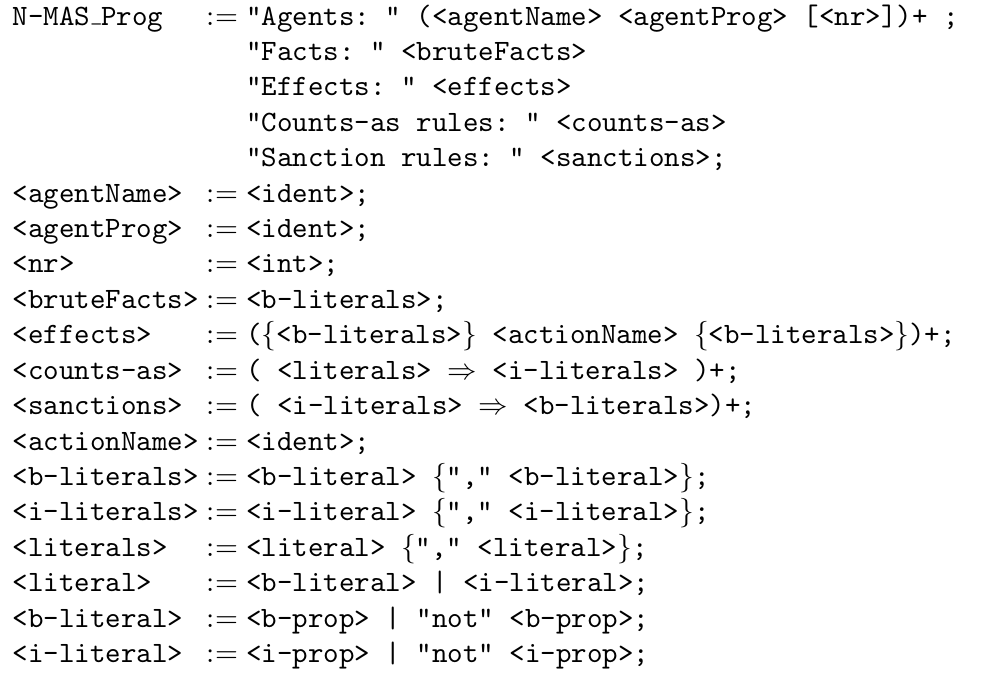
\includegraphics[width=0.8\linewidth]{figure/masprogram.png} 
  \caption{Linguagem para descrever um programa de multiagentes normativos com a possibilidade de violações e sanções na notação EBNF segundo o texto \cite{dastaniframework}. Nesta notação, $<ident>$ é usado para denotar uma \textit{string} e $<int>$ inteiros. Os termos $<b-prop>$ e $<i-prop>$ são usados para designar dois tipos de conjuntos de proposições que são disjuntos entre si}
  \label{descreveprograma}
\end{figure}

Os \textit{Facts} implementados em forma de \textit{brute facts} definem os estados iniciais do sistema dentro de um ambiente compartilhado por todos os agentes. O termo \textit{Effects}, implementado por meio de $effects$ define como se dá a transição de estados do sistema. A tag $<actionName>$ representa os eventos que geram transição dos estados. Uma norma, portanto, é definida em termos de \textit{Counts\_as rules}. O termo $<counts-as>$ aponta para transição entre $<literals>$ e $<i-literals>$. Isso representa os fatos que resultam em violações. Portanto, em \cite{dastaniframework} as normas são descritas por intermédio de suas violações. Violação, dentro deste contexto, é dado como o descumprimento da norma 
\cite{ontologynormative}.

O termo \textit{Sanction Rules} aponta para $<sanctions>$ e esses, por sua vez, para a transição entre $<i-literals>$ e $<b-literals>$ sendo que esses $<i-literals>$ advêm de \textit{Counts\_as Rules}. Assim sendo, \textit{Sanction Rules} define as consequências da violação. Essas consequências denotam caráter negativo ao agente tendo como foco uma natureza de ordem punitiva \cite{dastaniframework}. 

A figura \ref{exemploprograma} apresenta um programa escrito nessa linguagem. 

\begin{figure}[H]
  \centering
  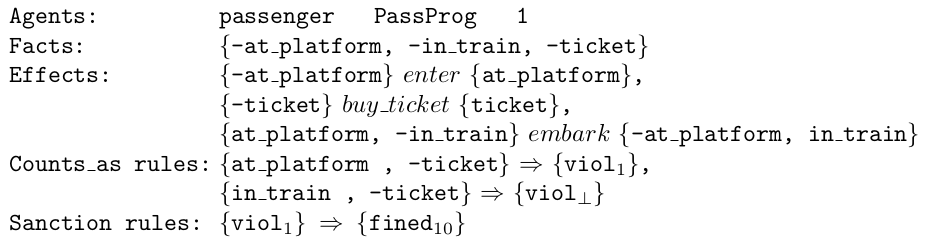
\includegraphics[width=0.8\linewidth]{figure/programdastani.png} 
  \caption{Um programa descrito na linguagem proposta neste estudo onde um agente representa um passageiro em uma estação de trem que pode entrar com ou sem um \textit{ticket} na plataforma e no trem \cite{dastaniframework}.}
  \label{exemploprograma}
\end{figure}

Esse programa contem um agente chamado de \textit{passenger} (especificações desse agente são detalhadas com maior rigor em \textit{PassProg}). Os \textit{Facts} deste programa são \textit{-at\_plataform} (agente não está na plataforma), \textit{-in\_train} (agente não está no trem) e \textit{-in\_ticket} (agente não possui o \textit{-in\_ticket}). As regras de \textit{Effects} apresentam dois $<actionName>$. O primeiro é denominado por \textit{enter} que tem por finalidade alternar entre os estados \textit{-at\_plataform} e \textit{at\_plataform}, 
ou seja, é uma ação onde o agente muda o estado de não está na plataforma para está na plataforma. O segundo estado é o \textit{buy\_ticket} que gera a transição entre os fatos \textit{-ticket} para \textit{ticket}, ou seja - na ocorrência \textit{buy\_ticket} o agente passa a ter um \textit{ticket} \cite{dastaniframework}.

O programa especifica duas regras em \textit{Counts\_as rules}. A primeira regra denota a ocorrência de uma violação para um agente que entra numa plataforma sem um \textit{ticket}. A segunda regra define que uma violação que acontece para o caso de um agente entrar em um trem sem um \textit{ticket} \cite{dastaniframework}.

O programa também define uma regra para \textit{Sanction rules}. Essa regra se aplica a $viol_1$, que - se verdade - então resulta no fato $fined_{10}$, cuja semântica denota um pagamento no valor de 10 unidades de moeda \cite{dastaniframework}.  


	\section{Riscos} \label{risksec}

		O primeiro estudo teórico sobre acidentes de trabalho se da no texto \cite{riskoldschool}. Essa pesquisa conclui que os erros em industria não podem ser definidos apenas nas falhas de 
humanos, mas sim como consequência de um comportamento global da instituição. Ainda dentro deste âmbito, esse comportamento advêm de uma forte pressão tendo em vista eficiência e otimização dos processos de produção \cite{riskoldschool} \cite{safety}.

Com base neste entendimento, o estudo \cite{safety} apresenta um arcabouço a fim de identificar as redes de causalidade que resultam em acidentes de trabalho. Assim sendo, a gestão de 
segurança se dá com base nos seguintes fatores; 
\begin{itemize}
    \item Políticas; \textit{leis, diretrizes, padrões e regras}
    \item Corporativo; \textit{regras, estratégias, politicas internas, gerenciamento}
    \item Projeto de Equipamentos de Trabalho; \textit{especificação, integração de segurança}
\end{itemize}

O item Política é mais relevante que os itens Corporativo e Projeto de Equipamentos de Trabalho. Esses dois últimos apresentam a mesma importância para uma estrutura de prevenção de acidentes 
bem sucedida. 

A primeira análise a ser feita diz respeito ao nível Corporativo-Projeto de Equipamentos de Trabalho. Muitas vezes a equipe adota atividades paliativas a fim de otimizar os processos de produção. Isso envolve assumir níveis de tolerância no que diz respeito ao desempenho e a segurança. Essa situação está dentro do conceito, para o arcabouço, de \textit{atividades
limites}, isso pois tratam de situações que trabalham no limiar com os riscos. Assim sendo, as decisões feitas pelo profissional podem resultar muito facilmente em acidentes ou incidentes \cite{safety}. 
Dentro desta perspectiva que se apresenta o ator \textit{BATU} - \textit{Boundary Activities Tolerated during Use} (Atividades Limites Toleradas Durante o Uso).

Existe dois tipos de \textit{BATU} que devem ser verificados tendo como base os processos de trabalho. Esses são; operacional e gerencial (administrativo - termo identificado no texto original; \textit{managerial}). Aquele faz referência as atividades relacionadas a melhoria da produtividade com o propósito de resultar em aumento das metas de produção, qualidade e segurança. Este diz respeito a decisões administrativas independentes dos processos operacionais mas que os impactam.

Outro conceito presente em \cite{safety} é o de \textit{Boundary Conditions Tolerated by Use} - \textit{BCTU} (Condições Limites Toleradas Durante o Uso). O termo condição faz referência a uma situação, um estado, circunstâncias externas às quais pessoas ou até mesmo entidades são afetados no que diz respeito a uma certa decisão. Assim sendo, \textit{BCTU} consiste em uma série de elementos e circunstâncias (ambiental, material, humana, produtos) que por conta de sua natureza ou de como se relaciona com as demais entidades e processos apresenta um certo potencial na geração de situações particulares, tendo em vista causas decorrentes de operações dinâmicas. Tanto os \textit{BATUs bem como os BCTUs} não podem ser analisados diretamente, mas devem ser analisados por intermédio das ações e escolhas dos operadores e dos atores que constituem esse trabalho \cite{safety}. 

Existe dois tipos de \textit{BCTU}. O primeiro consiste no \textit{BCTU} interno que se apresenta como uma concepção global de trabalhos e situações no que tange as relações de política da empresa. Nesta concepção, \textit{BCTU} interno faz referência as diferenças hierarquias em termos de nível e decisões centrais. Em contraste com esse ponto, o \textit{BCTU} externo aponta para o projeto da instalação. Como resultado, há o surgimento de quatro derivações, que são; soluções de segurança - funções de segurança (diz respeito as questões que podem fazer com que um dispositivo de segurança venha a falhar), soluções técnicas - requisições de trabalho (quando as soluções técnicas são incompatíveis com as requisições de trabalho), modelo de projeto - modelo de instalação (se da quando a solução final não é ótima ou está degradada quando comparada com a solução inicial) e condições nominais preventivos - condições reais de operação
\cite{safety}.

As relações entre \textit{BATU}s e \textit{BCTU}s são dinâmicas e são dependentes do processo. Para exemplificar, pode-se considerar o seguinte cenário; O projeto de uma máquina de dobra de papel obriga o operador a adotar uma dada posição que o faz assumir riscos para acessar determinados pontos da máquina.  Assim sendo, as escolhas do projeto da máquina (relacionada ao \textit{BCTU}) não levam em consideração todos os aspectos relacionados a dinâmica profissional-máquina fazendo o que o profissional envolvido tenha que atuar dentro de um certo intervalo de tolerância no que diz respeito a segurança profissional \textit{BATU}.
		

	\section{Lógica Modal} \label{logic}

		A lógica modal consiste em uma linguagem para tratar proposições que necessariamente ocorrem e proposições que possivelmente ocorrem. As proposições dadas como necessárias são aquelas que necessariamente são verdade. Por exemplo, A água sobre 1 atm e entre 0,1 ºC - 99 ºC se apresenta no estado líquido. O conceito de possibilidade é totalmente dependente do conceito de necessidade. Isso pois uma proposição possível é aquela que necessariamente não é falsa \cite{modallogic}. 

A lógica modal é do tipo \textbf{K} e isso significa que nela está condita símbolos $ \sim $ para não, $ \rightarrow$ para "se ... então" e $\Box$ para "Isto é necessário". 

De \textbf{K} e $\Box$, tem-se as seguintes regras;

Sendo que $isTheorem(A,\textbf{K})$ representa "Se A é teorema de \textbf{K}". 

\begin{equation} 
isTheorem(A,\textbf{K}) \rightarrow \Box A
\end{equation}
\label{ktheorema}

\begin{equation} 
 \Box (A \rightarrow B) \rightarrow (\Box A \rightarrow \Box B) 
\end{equation}
\label{boxdist}

O operador $\Diamond$ apresenta o seguinte correspondente semântico; "Isto é possível". A relação entre $\Box$ e $\Diamond$ é dada pela regra que se segue.

\begin{equation} 
 \Diamond A = \sim\Box\sim A
\end{equation}
\label{dianotboxnota}

As relações a seguir apresentam outras regras válidas para essa lógica;

\begin{equation} 
 \Box (A \wedge B)  \rightarrow \Box A \wedge \Box B
\end{equation}
\label{boxand}

\begin{equation} 
 \Box A \vee \Box B \rightarrow \Box (A \vee B)
\end{equation}
\label{boxaor}

\begin{equation} 
 \Box A \rightarrow A
\end{equation}
\label{boxtoa}

\begin{equation} 
    \Box A \rightarrow \Box\Box A
\end{equation}
\label{aboxbox}

\begin{equation} 
    \Diamond A \rightarrow \Box\Diamond A
\end{equation}
\label{diaaboxdiaa}

\begin{equation} 
    \Box\Box...\Box = \Box
\end{equation}
\label{alotbox}

\begin{equation} 
    \Diamond\Diamond...\Diamond = \Diamond
\end{equation}
\label{diamont}

\begin{equation} 
    A \rightarrow \Box\Diamond A
\end{equation}
\label{diamont}


\chapter{Metodologia}
\label{chap:metod}

	ofkhgojfgpoksdogśgp[sigṕwgs


    \section{Levantamento de Requisitos} 
    
        O interesse desse estudo reside conceber um modelo que possa ser aplicado a uma certa classe de problemas. Assim sendo é importante que os requisitos não sejam focados com base em casos específicos mas que resultem em algo com certa capacidade de generalização. Nessa linha de raciocínio os requisitos são necessariamente os objetivos propostos nesse estudo. 

Os objetivos desse estudo não definem um caso de estudo em específico, mas estruturam o que deve ser modelado e quais são os compomentes que devem necessariamente fazer parte desse sistema. A natureza desses requisitos é estática, ou seja - uma ves que foram definidos (processo obtido na busca do que se deseja investigar), esses elementos não foram modificados. 

Outro ponto interessante reside no fato de que, em muitos casos, os requisitos não são claramente definidos (diversos são os fatores que ocasionam nisso, mas em Engenharia de \textit{Software} isso se dá tendo em vista uma certa falta de comunicação entre o implementador e o solicitante) \cite{softwareeng}. Contudo, esse problema não acontece nesse estudo de caso porque os requisitos são definidos pelos próprios implementadores e os termos são construidos em um vocabulário comum para toda comunidade acadêmica da ciência da computação (agentes, sma, normas, violações, objetivos e entre outros). 
 
 
    \section{Levantamento de Requisitos} 
    
        O interesse desse estudo reside conceber um modelo que possa ser aplicado a uma certa classe de problemas. Assim sendo é importante que os requisitos não sejam focados com base em casos específicos mas que resultem em algo com certa capacidade de generalização. Nessa linha de raciocínio os requisitos são necessariamente os objetivos propostos nesse estudo. 

Os objetivos desse estudo não definem um caso de estudo em específico, mas estruturam o que deve ser modelado e quais são os compomentes que devem necessariamente fazer parte desse sistema. A natureza desses requisitos é estática, ou seja - uma ves que foram definidos (processo obtido na busca do que se deseja investigar), esses elementos não foram modificados. 

Outro ponto interessante reside no fato de que, em muitos casos, os requisitos não são claramente definidos (diversos são os fatores que ocasionam nisso, mas em Engenharia de \textit{Software} isso se dá tendo em vista uma certa falta de comunicação entre o implementador e o solicitante) \cite{softwareeng}. Contudo, esse problema não acontece nesse estudo de caso porque os requisitos são definidos pelos próprios implementadores e os termos são construidos em um vocabulário comum para toda comunidade acadêmica da ciência da computação (agentes, sma, normas, violações, objetivos e entre outros). 
 
    
    \section{Conceitualização} 
    
        Uma vez identificado quais são esses modelos e uma vez realizada as observações em campo, os pesquisadores formularam conceitos e relações interessantes para o estudo em análise. Feito isso, ocorre a etapa da adaptação, onde essas categorias são redefinidas em estruturas conceituais mais específicas com objetivo de construir um vocabulário especializado para as condições de interesse desse estudo. Como resultado dessa, os pesquisadores obtiveram uma lista de conceitos e suas relações específicas para representar cenários delineados pelos resultados das observações. 

A próxima etapa reside em escrever esses conceitos em algum tipo de formalismo. Nesse estudo, os pesquisadores optaram por usar teoria de conjuntos e lógica de predicados. Isso possibilitou estruturar o modelo em voga numa linguagem formal onde cada parte (conjunto, elemento e predicados) é um vocabulo com uma semântica clara. 

Os conjuntos são usados para representar um dado conceito. Os elementos de um conjunto representam os objetos atrelados ao conceito. Por exemplo, supondo que uma loja de Carros venda os seguintes veículos; \textit{Jetta}, \textit{Gol}, \textit{Uno}.
Nesta situação, o conceito de carro é representado pelo conjunto $C$ e os modelos são elementos do mesmo. Portanto, numa linguagem matemática formal tem-se a seguinte situação $C = \{Jetta,Gol,Uno\}$. 

Dentro do conceito matemático, uma relação é uma correspondência entre elementos de conjuntos não vazio, sendo dada por $R \subseteq  A \times B = \{(a,b)| a \in A \wedge b \in B \}$. A Lógica de Predicados foi usada para representar essas
relações.

O \textit{UML} também é uma ferramenta que foi usada para criar representações do modelo. O propósito disto consiste nos seguintes aspectos; apresentar perspectiva global do modelo, definir melhor os critérios existenciais (agregação, composição),
tornar o processo de apresentação mais didático e aproxima-lo de mecanismos de implementação (ex. linguagens de programação).  
 

\chapter{Resultados}
\label{chap:resul}

	Esse capítulo tem como finalidade exibir os resultados obtidos ao longo do estudo dessa pesquisa. Os resultados presentes em \ref{resrevisaoexploratoria} são referentes a etapa metodológica descrita ta seção \ref{revexpanalcamp}, já os resultados presentes em \ref{estconceitual} são consequências da descrição metodológica apresentada em \ref{modconceitual}. A seção \ref{introdutorycase} mostra a aplicação deste modelo para um caso simples com a finalidade de introduzir didaticamente o leitor à estrutura do modelo. 
	
	\section{Estrutura Conceitual}

	Essa parte do texto é estruturado em; Módulo (exibe informações sobre os módulos e os conceitos neles contidos), Predicados (apresenta os predicados e justifica a sua existência) e as regras (exibe as regras e explica porque sua existência dentro do modelo é necessário). 

		\subsection{Módulos} 
			\label{mods}			
			Os conjuntos que representam os conceitos são organizados em  módulos. Isso ocorre porque muitos conceitos apresentam similariedades, sendo razoavel conceber uma taxonomia desses conjuntos organizando-os em conjuntos maiores. A figura \ref{module} apresenta a estrutura de módulos (a fim de evitar poluição visual, as relações serão apresentadas em outra figura). 

\begin{figure}[H]
  \centering
  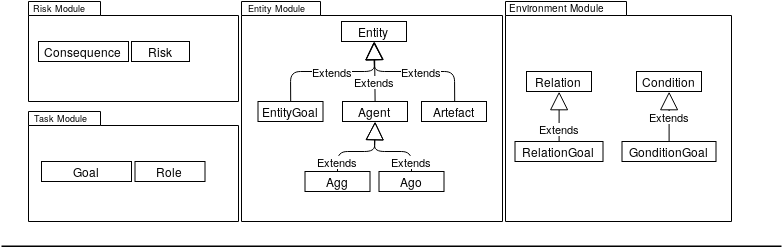
\includegraphics[width=1\linewidth]{figure/Module.png} 
  \caption{A estrutura geral das classes do modelo}
  \label{module}
\end{figure}

Assim sendo, assumindo que existe $\Omega_{Model}$ (um conjunto global onde todos os outros conjuntos do modelo estão contidos nele), os módulos são representados da seguinte maneira; 

\begin{equation} 
    \Omega_{Model} = \{ M_{Risk}, M_{Task}, M_{Entity}, M_{Environment}\}
\end{equation}
\label{modules}


O mundo sobre o qual este modelo pretende representar trabalha com o fato de que tanto agentes bem como artefatos possuem algumas propriedades em comum, que é; existem, ocupam lugar no espaço, estão sujeitos ao tempo, apresentam estados e participam de processos. Essa premissa possue os seus fundamentos alicerçados em \ref{agent} e \ref{artefact} e isso será demonstrado com maior rigor no texto que se segue. Tendo em vista o ocorrência de certos conceitos necessários para lidar com essas questões, se fez necessário definir um módulo de entidades para agrupa-los em uma estrutura única. Esse módulo é composto pelos seguintes conceitos;

\begin{equation} 
M_{Entity} = \{ Entity, Agent, Artefact, EntityGoal, Agg, Ago\}
\end{equation}\label{modent}

\textbf{Entity} - O termo entidade é sujeito a profundos debates filosóficos, porém neste texto o termo é usado para referenciar uma "coisa" que pode ser identificada, como uma pessoa, companhia ou um evento \cite{entity}. É dado que as propriedades anteriormente mencionadas caracterizam as "coisas" que podem ser identificadas, logo entidades. É digno de nota a existência de entidades que não se adequam a todas essas propriedades. Contudo, essas propriedades fazem referência ao que se caracteriza por entidade respeitando o conceito padrão \cite{entity} e restringindo para o escopo deste modelo. Isso contempla tanto os agentes assim como artefatos, como fica claro na relação \ref{defineentity}. O texto a seguir demonstra como essas propriedades se aplicam a agentes e a artefatos (se isso ficar demonstrado, logo fica demonstrado que são entidades).

\textit{Existe -} Dado como quantificador, se há um ou mais, então existe. Assim sendo, tanto agentes como artefatos existem porque, dentro da representação, ambos fazem referência a coisa que correspondem a um ou mais. 

\textit{Ocupa lugar no espaço, estão sujeitos ao tempo - } Como definido em \ref{agent} e \ref{artefact}, ambos são situados em ambientes. 
Isso possibilita inferir que se faz necessário a presença de um conceito que se apresente como uma propriedade de estado para agentes e artefatos. Um ambiente, no contexto onde os agentes e artefatos são usados para representar atividades das pessoas, condiz com a relação de espaço e tempo. 

\textit{Participa de Processos -} Processos podem constituir entidades bem como entidades necessariamente constituem processos por intermédio a ação que aquelas manifestam nesses. No que se verifica ao primeiro caso, é possível usar o ser humano como exemplo - onde
a entidade humano é formulada por uma série de processos bio-químicos. Sobre o segundo caso, relações climáticas exemplificam isso, onde a água é uma entidade presente em processos termodinâmicos. 

\textit{Apresenta estados -} O fato de que artefatos bem como agentes apresentam atributos (que podem mudar e podem assumir diferentes valores no que tange aos eventos externos e internos), então ambos também apresentam a concepção de estados (sendo esse termo usado diretamente em certos pontos dos textos presentes tanto em \ref{agent} \ref{artefact}). 


\begin{equation} \label{defineentity} 
( Agent \cup Artefact ) \subset Entity
\end{equation}

\textbf{Agent} - Esse estudo adota a definição de agentes presentes no primeiro parágrafo da seção \ref{agent}. Isso implica entidades autônomas, ou seja -que apresenta a capacidade de agir por si mesma quando diante de condições onde isso é necessário. A seção \ref{agent}, apresenta o conceito de agentes inteligentes e esse mesmo conceito é adotado neste modelo. 

Não é preocupação deste estudo delimitar as representações do agente bem como definir algoritmos para verificar como se da as relações de tomada de decisão. Assim sendo, fica em aberto para o modelador definir como se dá os processos de tomada de decisão, estados internos e modelos de representação que serão usados para definir o comportando do agente. 

\textbf{Artefact} - são entidade que existem para que os agentes possam cumprir com os seus objetivos e que apresentam interface de uso, instruções de operação, funcionalidade e estrutura-comportamento. Essas entidades não são orientados a objetivos e 
não apresentam capacidade de comunicação como definido na seção \ref{artefact}. Predicados que contemplam esses aspectos do artefato serão apresentados mais adiante ao decorrer do texto. 

Os agentes são autônomos e orientados a objetivos sendo esses dois elementos descaracterizantes do que se defini como por artefato. Logo, apesar de agentes e artefatos serem entidades, não é possível existir um agente que seja artefato ou um artefato que seja agente, o que é dado por \ref{agentsartefactvoid}. 

\begin{equation} \label{agentsartefactvoid}
    Agent \cap Artefact = \{ \emptyset \}
\end{equation}


\textbf{EntityGoal} - Condiz a subconjuntos de \textbf{Entity} que, por intermédio de um predicado que será apresentado posteriormente, se relacionam com elementos do conjunto \textbf{Goal} (representam os objetivos). Assim sendo, consiste nas entidades necessárias que devem estar presentes no ato da execução de um certo objetivo para que este possa ser alcançado. Para exemplificar é possível conceber o seguinte cenário; 

\textbf{Exemplo da Redação:} "O Professor Aristóteles definiu uma atividade; Escrever uma redação sobre o livro Metafísica. Para isso, o aluno Alexandre o Grande deve escrever um dado texto, deve ler o livro sobre o tópico em definido, deve pegar uma folha, deve pegar um lápis e escrever a redação".  


Neste modelo, esse cenário pode ser especificado da seguinte forma; $E = \{aristoteles, alexadre, folha, lapis, livro\}$, em termos de objetivo (esse conceito será descrito com maior detalhe no texto em diante) há três $G = \{ g_0, g_1,g_2\}$  onde $g_0$ corresponde ao ato do professor definir a atividade, $g_1$ corresponde ao ato de ler o livro e $g_2$ ao ato de escrever a redação. Então, é possível 
definir três subconjuntos de $E$, esses são os conjuntos \textbf{EntityGoal}, $E_g = \{ eg_{0}, eg_{1}, eg_{2} \}$, onde $eg_{0} = \{ aristoteles \}$ $eg_{1} = \{ alexandre, livro\}$ e $eg_{2} = \{ aluno, folha, lapis \}$. Em termos de relação, que será melhor trabalhado 
em partes futuras deste texto, considera-se que $eg_0$ se relaciona com $g_0$, $eg_1$ se relaciona com $g_1$ e $eg_2$ com $g_2$.

\textbf{Agg, Ago} - ambos correspondem ao conjunto de agentes que atingiram um determinado objetivo. Contudo, \textbf{Agg} faz referência aos gentes que atingiram o objetivo sem serem obrigados a isso, e \textbf{Ago} condiz aos agentes que atingiram o objetivo sendo obrigados a isso. Em um primeiro momento essa diferença para ser desnecessária, mas é relevante para criação de regras que serão apresentadas futuramente. A necessidade deste conjunto pode por ser demonstrada com o \textbf{Exemplo da Redação}, pois Alexandre e Aristóteles são obrigados a alcançar os objetivos. Então, é definido por $Ago = \{ ago_0, ago_1, ago_1 \}$ onde $ago_0 = \{ \emptyset \}$ , $ago_1 = \{ \emptyset \}$ e $ago_2 = \{ \emptyset \}$. Ao atingir $g_0$ o $ago_o = \{ artistoteles\}$ pois o professor cumpriu com o objetivo de passar a atividade. O mesmo ocorre para $ag_1$, $g_1$ e para $ag_2$, $g_2$.


\textbf{O Módulo de Atividades} - \textit{Task Module} representado por $M_{Task}$ condiz com os conceitos relacionados aos obetivos que devem ser atingidos bem como aos papéis que são assumidos pelos agentes.
\begin{equation}
    M_{Task} = \{ Goal, GoalPreRequisite, Role \}
\end{equation}

\textbf{Goal} - faz referência aos objetivos que devem ser atingidos pelos agentes. Os fundamentos semânticos deste conjunto está presente na seção \ref{sma} mais especificamente na subseção \ref{moiseformalizesma}. Neste modelo, um objetivo é descrito em termos de $eg$ e $rg$ (conjuntos de relacionamentos, será explicado com maior detalhes no texto adiante), que são as entidades e os relacionamentos (será explicado) que devem ser ser feitos para que o objetivo possa ser dado como concluído. Com o propósito de explorar com maior granularidade as relações entre o agente e o objetivo, neste modelo o conceito de missão foi removido. Como será apresentado posteriormente, as relações deônticas entre os papéis se dão com o objetivo e não com a missão. O estudo presente no \textit{MOISE+} faz uso de grafos para representar objetivos-subobjetivos. Esse modelo não importou a estrutura em grafos para descrever o comportamento de objetivos. 

\textbf{Role} - apresenta o papel que um agente pode adotar dentro de um \textit{SMA}. Esse conceito também é importado no \textit{MOISE+} 
\ref{moiseformalizesma} e define as relações deonticas entre os agentes e os objetivos. Para exemplificar, pode-se considerar o \textbf{Exemplo da Redação} onde existe dois agentes $Agent = \{ aristoteles, alexandre \}$, existe dois papéis $Role = \{ professor, aluno\}$. Neste caso, o agente $aristoteles$ é o $professor$ e o agente $alexandre$ é o $aluno$.

\textbf{O Módulo de Ambiente} - \textit{Environment Module} - consiste em conjuntos que representam relações e condições ambientes, esses são;

\begin{equation}
    M_{Environment} = \{ Relation, Condition, Circumstance, ReationGoal, ConditionGoal \}
\end{equation}

\textbf{Relation} - Uma entidade estabelece relações com outras entidades ao seu redor \cite{entity}. No modelo proposto neste texto, 
os pesquisadores optaram por definir um conjunto que representa essas relações. Os pesquisadores optaram por um conjunto para representar
os relacionamentos entre as entidades porque isso possibilita identifica-los. Isso facilita o desenvolvimento de raciocínios. O uso 
dos relacionamentos podem ser exemplificado por meio do \textbf{Exemplo da Redação}. Ao definir uma atividade, o professor Aristóteles
, que é uma entidade, estabeleceu uma relação com o seu aluno Alexandre, representado aqui por $relAristotelesAlexandre$. Para cumprir com essa tarefa o aluno teve de ler o livro - $relAlexandreLivro$, teve de pegar uma folha - $relAlexandreFolha$, teve de pegar um lápis $relAlexandreLapis$ e teve de escrever a redação o que implica em uma relação entre lápis e folha $relLapisFolha$. Portanto, o conjunto de relacionamentos se dá da seguinte maneira;

\begin{eqnarray}\label{Environment}\nonumber
    M_{Environment} = \{ relAristotelesAlexandre, relAlexandreFolha, relAlexandreLivro, \\ \nonumber
     relAlexandreLapis, relLapisFolha \}
\end{eqnarray}

Obviamente, cada entidade do grupo \textit{Relation} tem uma vínculo com elementos do grupo \textit{Entity}, como por exemplo $relAlexandreFolha$ apresenta um dado vinculo com as entidades $Alexandre$ e $Folha$. Há um predicado que trata disto e será exibido posteriormente. Assim como o conjunto $EntityGoal$, existe relacionamentos que devem estar presentes para que dados objetivos possam ser atingidos, revelando - portanto - a necessidade de um conjunto para representar esse tipo de situação, que neste caso é $RelationGoal$. O exemplo em análise é descrito por três objetivos. O objetivo $g_0$ corresponde ao ato  do professor definir a atividade. Esse objetivo não pode ser cumprido sem relacionamento $relAristotelesAlexandre$. Portanto, existe $rg_0$ associado a $g_0$ onde $rg_0 = \{ relAristotelesAlexandre \}$ e que $rg_0 \subset RelationGoal$. O conjunto $g_1$ está relacionado com $rg_1$ e esse, por sua vez, é composto por $\{ relAlexandreFolha\}$. O conjunto $g_2$ está relacionado com $rg_2$ e os elementos correspondem a $\{ relAlexandreLapis, relLapisFolha, relAlexandreFolha\}$.

\textbf{Condition} - Esse conjunto representa as condições que devem ser mantidas para que um dado objetivo possa ser alcançado. Em analogia a $EntityGoal$ e a $RelationGoal$, há um conjunto denominado de $ConditionGoal$ que define essas condições para os objetivos. Para exemplificar o uso deste conjunto é possível considerar o \textbf{Exemplo da Redação}. Com certeza nenhum dos três objetivos se tornam viáveis se não houver luz suficiente para que todos possam ver. O ambiente deve ser mantido em um certo silêncio, do contrário não há possibilidade do professor e do aluno exercer suas atividades intelectuais. Assim sendo é possível definir duas entidades; $Condition = \{ luz,silencio \}$. Ambas as condições são válidas para todos os objetivos (para esse
exemplo), portanto existe um $cg_1 = \{ luz,silencio \} | CondtionGoal = \{ cg_1 \}$, sendo que $cg_1$ estabelece relações com 
$g_0$, $g_1$ e $g_2$.

Certos relacionamentos, que serão apresentados com maior riqueza de detalhes mais adiante, exigem definir uma certa abstração entre \textbf{Condition} e \textbf{Relation}. Assim sendo, os pesquisadores assumem a existência de um conjunto \textbf{Circumstance} que é dado pela seguinte relação; 

\begin{equation}
    Circumstance = \{ Relation, Condition \} |  Relation \cap Condition = \{ \emptyset \}
\end{equation}


\textbf{Módulo de Risco} - \textit{Risk Module} contem conjuntos que correspondem a conceitos relacionados a temática da segurança.
O módulo de risco é dado pela relação que se segue;

\begin{equation}
    M_{Risk} = \{ Risk, Consequence \}
\end{equation}

\textbf{Risk} - Na seção \ref{risksec} o termo risco é usado para referenciar a um evento que apresenta um potencial de ocorrer e que gera consequências negativas as pessoas associadas quando acontece. Para exemplificar pode-se considerar uma condição onde um eletricista está trocando um disjuntor de um quadro elétrico. Nesse processo, o eletricista está sujeito ao risco de ser eletrocutado. Essas consequências negativas também são representadas por um conjunto, e esse é \textbf{Consequence}. O uso deste conjunto pode ser apresentado utilizando esse mesmo exemplo do eletricista, pois a consequência de se submeter a um evento desses implica morte (nem sempre é assim, mas para efeitos didáticos pode-se considerar que o quadro elétrico é de certa potência que a morte é certa para o profissional que for eletrocutado).
		
		\subsection{Predicados} 
			\label{predic}
			O predicado $thereIsRelation(r_l,e_i,e_k) | r_l \in Relation \wedge  e_i, e_k \in Entity$ é usado para tratar as questões de identificar a relação entre duas entidades com a sua relação. Esse predicado se lê da seguinte forma: O relacionamento $r_l$ possui a entidade $e_i$ e a entidade $e_k$. Para demonstrar como se dá o uso desse predicado pode-se considerar o \textbf{Exemplo da Redação}. A entidade $alexandre$ apresenta uma relação com $folha$ que é identificada como $relAlexandreFolha$. Portanto, com o predicado, a representação 
fica; $thereIsRelation(relAlexandreFolha,alexandre,folha)$

O predicado $hasRole(ag_n,\rho_m) | ag_n \in Agent \wedge \rho_m \in Role$ que tem sua origem nos estudos do \textit{MOISE+} onde 
cada agente tem uma função dentro do contexto do \textit{SMA}. Esse predicado se lê da seguinte forma: O agente $ag_n$ tem um
papel $\rho_m$. Usando o \textbf{Exemplo da Redação} tem-se o seguinte: $hasRole(artistoteles,professor)$. 

O predicado $hasObligation(\rho_m,g_j) | \rho_m \in Role, g_j \in Goal $ tem suas origens nos estudos da lógica deôntica também 
presentes no modelo \textit{MOISE+}. Esse predicado pode ser lido da seguinte maneira: O agente que assumir o papel $\rho_m$ tem a 
obrigação de concluir o objetivo $g_j$. No exemplo padrão deste texto (\textbf{Exemplo da Redação}), o primeiro objetivo é uma
obrigação do professor, portanto: $hasObligation(professor,g_0)$

O predicado $hasPermission(\rho_m, g_j) | \rho_m \in Role, g_j \in Goal $ também está associado aos estudos da lógica deôntica
relacionada ao \textit{MOISE+}. A leitura se dá desta maneia: O agente que $\rho_m$ tem a permissão de concluir o objetivo $g_j$.
Usando o exemplo padrão como base, onde $professor$ tem a obrigação para executar $g_0$, então também tem permissão (isso
será melhor explicado em uma regra que será apresentada mais tarde). Portanto; $hasPermission(professor,g_0)$.  

O predicado $isReached(g_k) | g_k \in Goal $ Todos os agentes, que eram obrigados a concluir o objetivo $g_k$, concluíram. A 
existência desse predicado se dá devido ao fato de que em certos raciocínios é necessário identificar que um dado objetivo 
foi atingido. 

O predicado $stopIn(g_n, ag_m) | g_n \in Goal, ag_m \in Agent$ apresenta a seguinte leitura: Toda a atividade foi encerrada no
objetivo $g_n$ por uma ação associada ao agente $ag_m$. Para certos raciocínios se faz necessário identificar o encerramento
das atividades como um todo e por quem isso aconteceu. Em certos casos não há a necessidade de identificar o agente $ag_m$. Para
isso há uma outra versão deste mesmo predicado escrito da seguinte forma: $stopIn(g_n)$ e sua semântica indica que a atividade 
foi encerrada do objetivo $g_n$.

O predicado $nextGoal(g_i,g_j) |g_i, g_j \in Goal$ possui a seguinte semântica: O objetivo $g_i$ tem um próximo o objetivo que 
é $g_j$. Sua necessidade advêm do fato de que este modelo trabalha os mesmos conceitos presentes em \textit{MOISE+} porém sobre
uma abordagem diferente. Em vez de usar estrutura de super-sub objetivos e definindo operadores de série e paralelo, os objetivos 
não possuem estruturas e suas relações se dão por um objetivo apontado para o próximo. Então, para exemplificar pode-se 
considerar uma atividade descrita por quatro objetivos, sendo que $g_0$ é pré-requisito para $g_1$ e $g_2$. Em contrapartida
$g_3$ só começar a ser atingido depois da finalização de $g_1$ e $g_2$. Assim sendo, na linguagem proposta neste estudo, 
esse problema é escrito da seguinte forma: $nextGoal(g_0,g_1), nextGoal(g_0,g_2), nextGoal(g_1,g_3), nextGoal(g_2,g_3)$.

O predicado $hasCondition(g_i,cg_n) | g_i \in Goal, cg_n \subset GoalCondition$ é lido da seguinte forma: O objetivo $g_i$ só pode 
ser iniciado se todas as condições presentes em $cg_n$ estiverem presentes quando o agente iniciar a tentativa de alcança-lo. 
O uso deste predicado pode ser exemplificado por meio do exemplo padrão. Tendo em vista que o objetivo $g_0$ pode começar apenas 
se as condições $cg_1 = \{ luz, silencio \}$, então para este caso, é possível escrever o seguinte predicado: $hasCondition(g_0,cg_1)$.

O predicado $hasEntity(g_i,eg_m) | g_i \in Goal, eg_m \subset EntityGoal $ é lido da seguinte forma: Para que o objetivo $g_i$ seja atingido, as entidades presentes em $eg_m$ devem estar presentes. O propósito deste predicado reside na necessidade de identificar quais são as entidades que devem estar presentes para que um dado objetivo possa ser executado. No \textbf{Exemplo da Redação}, um objetivo $g_2$ só pode ser 
atingido se as entidades $eg_2 = \{ aluno, folha, lapis\}$ estiverem presentes. Para essa situação, esse predicado é escrito da 
seguinte forma $hasEntity(g_2,eg_2)$.

O predicado $hasEntity(g_i,rg_m) | g_i \in Goal \wedge rg_m \subset RelationGoal $ é lido da seguinte forma: Para que o objetivo $g_i$
seja atingido se faz necessário a realização de todos os relacionamentos contidos em $rg_m$. Dentro do exemplo padrão, o objetivo 
$g_2$ só pode ser atingido se os relacionamentos $rg_2$ estiverem presentes. Portando, a especificação para esse situação é escrita
da seguinte forma: $hasRelagion(g_2,rg_2)$.

O predicado $isPresent(X) | X = cg_n \vee X = c_k \vee  X = rg_k \vee X = r_k \vee X = eg_k \vee X = e_k $. Esse predicado é lido 
da seguinte forma: $X$ está presente neste instante. Em alguns raciocínios e de importância verificar se um elemento ou um conjunto
de elementos está presente durante a tentativa de um dado agente tentar executar algum objetivo.

O predicado $tryReach(ag_i,g_j) | ag_i \in Agent \wedge g_j \in Goal $ é lido da seguinte forma: Um dado agente $ag_i$ está tentando 
atingir o objetivo $g_j$. Para algumas situações é de crucial importância identificar quando um agente está tentando atingir um 
dado objetivo, fazendo-se necessário a existência de um predicado apenas para esse propósito. Para exemplificar pode-se considerar 
o exemplo presente no quadro do professor Aristóteles com o seu aluno Alexandre. Para que o professor $Aristoteles$ possa alcançar 
o objetivo $g_0$, ele precisa tentar fazer isso. Neste modelo, essa situação é representada da seguinte maneira: $tryReach(aristoteles,g_0)$.
Seguindo a linha desse predicado, há também o $ableTryReach(ag_i,g_j) | ag_i \in Agent \wedge g_j \in Goal$ cuja semântica expressa que o agente $ag_i$ está habilitado para tentar buscar o objetivo $g_j$. Contudo, não significa que o agente fará o correspondente de $tryReach(ag_i,g_j)$. O que definirá a transição de estado: habilitado a alcançar um dado objetivo para o estado: tentando alcançar um dado objetivo consiste em estados internos do agente. Contudo, não é do interesse deste estudo aprofundar na dinâmica do agente em si - deixando esse processo em aberto para o programador decidir como resolverá essa questão.

O predicado $ violationCondition(ag_i,g_j,c_k) $ sendo que $ ag_i \in Agent \wedge g_k \in Goal \wedge c_k \in Condition \wedge c_k  \in cg_n \wedge cg_n \subset ConditionGoal $. Esse predicado deve ser lido da seguinte maneira: O agente $ag_i$ comente uma violação de condição no objetivo $g_j$ por tentar realizar uma determinada atividade em que a condição $c_k$ era essencial porém não estava presente. Os fundamentos deste predicado está vinculado com a seção \ref{normasdastani}. No modelo em \ref{normasdastani} para representar aspectos normativos dos agentes, a regra do tipo \textit{Count-as} apresenta quais são as circunstâncias que ocasionam numa violação. Esse predicado cumpre com esse propósito para o conjunto \textbf{Conditions}. Para exemplificar, no \textbf{Exemplo da Redação}, se o professor Aristóteles lecionar sem que haja luz suficiente para isso, então ele cometeu uma violação de condição caracterizada da seguinte maneira: $violationCondition(aristoteles,g_0,luz)$

O predicado $ violationRelation(ag_i,g_j,r_k) $ sendo que $ ag_i \in Agent \wedge g_k \in Goal \wedge c_k \in relation \wedge r_k  \in rg_n \wedge rg_n \subset RelationCondition $. Esse predicado possui a mesma situação presente em $ violationCondition(ag_i,g_j,c_k) $ contudo o foco diz respeito aos relacionamentos. A leitura se dá desta forma: O agente \textit{ag\_i} pratica uma violação de relação no objetivo $g_j$ por executar a atividade sem que a relação $r_k$ esteja presente. O uso deste predicado por ser feito considerando o exemplo em análise com a adição de uma breve descrição de uma situação que possa ocorrer que é o seguinte; A ponta do lápis que Alexandre tenta usar para escrever a redação está quebrada. Portanto, a relação \textit{relLapisFolha} não pode ser feita. Se o agente \textit{Alexandre} alcançar o objetivo $g_2$ sem ter as circunstancias necessárias para isso, então comente uma violação de relação sendo escrito da seguite forma: $violationRelation(alexandre,g_2,r_2)$.

O predicado $ violationEntity(ag_i,g_j,e_k) $ sendo que $ag_i \in Agent \wedge g_j \in Goal \wedge e_k \in Entity \wedge e_k \in eg_n \wedge eg_n \subset EntityGoal $. Esse predicado advêm das mesmas situações dos dois predicados a cima. A leitura deste predicado se dá da seguinte forma: O agente $ag_i$ cometeu uma violação por tentar alcançar o objetivo $g_j$ sem que a entidade $e_k$ esteja presente. No exemplo padrão o uso deste predicado consiste em Alexandre tentar executar $g_2$ sem ter a entidade lápis o que resulta no seguinte: $violationEntity(alexandre, g_2, lapis)$.

O predicado $ hasRisk(X, risk_j, cs_k) | risk_k \in Risk \wedge cs_k \in Consequence \wedge (X = c_k \vee X = r_k $ é baseado nos estudos 
presentes na seção \ref{risksec} e tem a finalidade definir os riscos associados a tentar executar algum atividade sem que 
$c_k$ ou $r_k$ esteja presente. Portanto, a leitura deste predicado é dada da seguinte forma; A ocorrência de uma violação 
onde $X$ está envolvido ocasiona em um evento associado ao $risk_j$ com a consequência $cs_k$. Ao explicar sobre o conjunto 
\textbf{Conequence}, foi dado um exemplo sobre um eletricista que tem o potencial de ser eletrocutado. Para esse exemplo, 
o uso deste predicado apresenta o seguinte formado: $hasRisk(relFerramentaIsolanteBarramento, eletrocutado, morte)$ que traduz
o ato do eletricista não efetuar o relacionamento de uma ferramenta isolante para entrar em contato com o barramento $relFerramentaIsolanteBarramento$, é eletrocutado e acaba se submetendo a $morte$ por conta disto.

O predicado $possibilityHappensBadEvent(r_l) | r_l \in Relation $ tem seus fundamentos associados ao estudo da lógica modal, presente na seção \ref{logic}, no operador $\Diamond$ cuja semântica denota possibilidade. Contudo, neste estudo esse termo apresenta o seguinte conceito semântico: há a possibilidade de acontecer um evento ruim associado ao risco $r_l$ vinculado ao agente que está associado a essa relação mesmo que esse agente não tenha cometido nenhum erro durante o procedimento. Esse predicado tem como por finalidade representar situações onde um evento ruim acontece não pelo erro do profissional diretamente associado a situação, mas sim por outras cadeias causais complexas de serem identificadas e justamente por isso são abstraídas por conceitos de aleatoriedades, idem possibilidades. Para exemplificar pode-se considerar a situação onde um eletricista de linha viva usa um bastão isolante para acessar um barramento altamente energizado. Contudo, esse bastão pode estar com isolamento comprometido. Em testes que deveriam ser feitos antes do eletricista fazer uso desta ferramenta, esse comportamento pode ser revelado eliminado qualquer possibilidade de que os riscos venham a se tornar eventos reais, pois se o bastão estiver em bom estado então o eletricista não se envolverá em um acidente por esse fator, se o bastão estiver em mal estado - isso será identificado e a ferramenta será adequadamente substituída. Contudo, considerando um cenário onde por negligencia de profissionais a medição não é feita, surge uma possibilidade do isolamento estar comprometido. Essa situação torna verdade o seguinte predicado $possibilityHappensBadEvent(relBastaoBarramento)$.

O predicado $affectsOtherRelations(r_k,r_n) | \{ r_k, r_n\} \subset Relation $ trabalha em conjunto $possibilityHappensBadEvent(r_l)$. Esse predicado se lê da seguinte forma: Se $r_k$ não foi realizado, ou se for realizado de forma inapropriada, isso afeta  $r_n$ tornando verdade 
$possibilityHappensBadEvent(r_n)$. Ambos são importantes em raciocínios onde se deseja mostrar que a não execução de um dada relação 
não gera consequências negativas imediatas a ninguém, mas resulta em consequências futuras inclusive sobre pessoas que não compartilham 
da mesma situação. No exemplo do eletricista, a relação $relBastaoBarramento$ e afetada pela não execução da relação $relBastaoMedidor$ 
que define a relação entre o aparelho medidor de corrente de fulga e o bastão isolante, sendo este evento escrito da seguinte maneira:
$affectsOtherRelations(relBastaoMedidor,relBastaoBarramento)$

O predicado $consequenceOfBadEvenet(g_k, ag_i,risk_k,cs_m)$ pode ser lido da seguinte maneira; ocorreu um evento ruim no 
objetivo $g_k$ associado ao agente $ag_i$ e associado ao risco $risk_k$ que atribuiu ao agente $ag_i$ consequências $cs_m$. Esse 
predicado tem por finalidade traduzir semanticamente as consequências ruins sobre alguém quando ocorre o pior caso. Sobre o exemplo 
do eletricista que acessa um barramento de alta tensão, esse predicado é escrito da seguinte forma: $consequenceOfBadEvenet(g_{acessoBarramento}, eleticista,eletrocutado,morte)$. Associado a isso há o predicado $happensBadEvent(r_m)$ cujo propósito define que um evento ruim aconteceu no relacionamento $r_m$.

O predicado $lastGoal(g_i,\rho_m) | g_i \in Goal, \rho_m \in Role $ apresenta um ultimo objetivo $g_i$ que deve ser alcançado 
por agentes com determinado papel $\rho_m$, Esse predicado tem sua existência justificada em certos raciocínios, que serão demonstrados 
mais adiante, onde esse tipo de informação é relevante.
			
		\subsection{Diagrama de Classes}
			Diferente da figura \ref{module}, o foco da figura \ref{classdiagrama} consiste em apresentar como se da a estrutura de classes e dos relacionamentos. Ambas situações poderiam ser representadas em uma única figura, contudo os pesquisadores decidiram por seccionar em duas a fim de tornar o processo mais didático. Por esse mesmo motivo não está apresentado neste \textit{UML} todas as classes e propriedades.  

\begin{figure}[H]
  \centering
  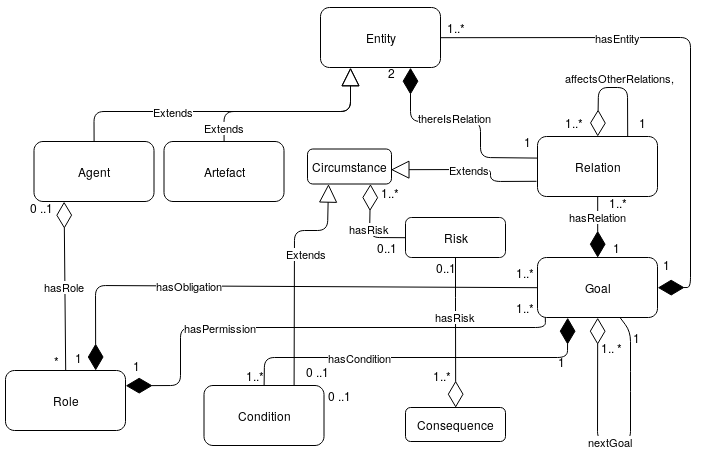
\includegraphics[width=1\linewidth]{figure/Class.png} 
  \caption{Diagrama de classes do Modelo }
  \label{classdiagrama}
\end{figure}

Uma vantagem deste tipo de diagrama em relação a representação por conjuntos consiste na ocorrência de uma sintaxe específica para tratar dois pontos relevantes dentro do contexto computacional: cardinalidade e relações existenciais. Um dos predicados interessantes de serem analisados, neste contexto, é \textit{adoptsRole} que define um relacionamento fracamente agregado entre \textit{Agent} e \textit{Role}. Isso, pois (dentro do escopo deste modelo) um agente pode existir sem ter um papel, portanto este não é um critério necessário para definir aquele. A cardinalidade se justifica tendo como base o fato de que um agente pode ter um ou mais papeis. 

As relações \textit{hasObligation}, \textit{hasPermission} se dão por meio de agregações fortes tendo vista que não há sentido para um papel $\rho$ existir sem que esteja vinculado a ao menos um objetivo. Como um papel se relaciona com diversos objetivos, os engenheiros adotaram a cardinalidade de $1$ para $1 .. *$.

Em \textit{UML} e relação de conjunto-subconjunto entre $Circumstance$ com $Relation$ e com $Condition$ é definida por meio de classes que possuem esses mesmos nomes. No \textit{UML}, as clases $Relation$ e $Condition$ são extensões da classe $Circumstance$. Dado essa situação, é possível representar a relação \textit{hasRisk} que ocorre entre $Circumstance$, $Relation$ e $Risk$ e isso é feito por meio do ternário entre essas classes. 

Um objetivo não pode ser definido sem saber quais são as entidades $Entity$, relações $Relation$ e consequências $Consequence$ necessários para que seja alcançado. Por isso os predicados $requiresCirc$,$requiresEntity$ e $hasRelation$ estabelecem composição forte de suas respectivas classes com $Goal$. Como um objetivo pode apontar para diversas instâncias dessas classes, os pesquisadores optaram - para cada uma das relações - trabalhar com a cardinalidade 
$1 - 1 .. *$.

No modelo proposto $Relation$ deve estar relacionada com duas entidades. Por esse motivo o predicado $possEntityRel$ faz composição forte com $Entity$ e a sua cardinalidade é dada $1 - 2$. 

A classe $Goal$ possui uma relação consigo mesma dada por $nextGoal$. Essa é uma agregação fraca, pois do contrários seria impossível haver uma única instância desta classe. Isso se deve ao fato de que a primeira instância necessitaria de uma instância de $Goal$ para existir. Contudo, como não há um elemento de $Goal$ antes do primeiro elemento de $Goal$, logo esse primeiro elemento não pode existir. Um objetivo poder ter como próximo um ou mais objetivos, justificando a ocorrência da cardinalidade $1 .. n$. 

O predicado $affectsRels$, por motivos similares a $nextGoal$ deve ter agregação fraca. Como uma relação pode afetar uma ou mais, a cardinalidade adequada para essa circunstância é dada pro $1$ - $1 ..*$


		\subsection{Regras}
			\label{regras}
			A Regra \ref{reldeonticrole} tem os fundamentos teóricos na lógica deôntica e em modelos como \textit{MOISE+}. Assim sendo, todas as relações de obrigação implicam relações de permissão. O que essa regra determina consiste no fato de que se um agente $a_j$ é obrigado a trabalhar sob o objetivo $g_j$, então esse agente também tem a permissão de trabalhar sobre o objetivo $g_j$ 

\begin{eqnarray}\label{reldeonticrole}
	hasObligation(\rho_m,g_j) \to hasPermission(\rho_m,g_j), \nonumber \\
    \rho_m \in Role \wedge g_j \in Goal
\end{eqnarray}

As regras \ref{conditionViol}, \ref{relationViol}, e \ref{entityViol} são fundamentadas em Seção \ref{normasdastani} onde o conceito do que pode ser feito é definido em termos das regras \textit{Count-as}. Essas regras determinam quais são os elementos que resultam em violação. Inspirando-se nesse tipo de estrutura são trabalhadas as referidas regras. 

A complexidade de estudo é extramente ampla, e com certeza existe mais tipos de violações do que as três consideradas a seguir, contudo optou-se por estudar essas violações porque são essenciais para os objetivos deste estudo. Outro questionamento que pode surgir consiste no por que definir três tipos de violações? Isso reside no fato de que essas violações resultam em consequências diferentes, por conta disto em um primeiro momento os engenheiros do modelo decidiram tratá-las em estruturas diferentes. 

A explicação das regras será feita sempre analisando-se a semântica do predicado que é implicado em relação aos estudos pelos quais elas se fundamentam. Partindo desta premissa, o entendimento da relação \ref{conditionViol} somente pode ser feito na ocorrência de uma  investigação sobre quais são os elementos que semanticamente correspondem ao predicado $conditionViol(ag_m,g_i,c_k)$. O primeiro ponto reside em verificar quais são as condições necessárias de $g_i$. Quem tem essa finalidade é o predicado $requiresCirc(g_i,c_k)$. Contudo, saber todas as condições não são o suficientes, pois a violação acontece na ausência de uma condição $c_k$ e isso deve ser verificado nesta relação de implicabilidade. Então se faz necessário considerar um predicado que analisa se $c_k$ está presente no ato da manutenção, e é com esse propósito que $isPresent(c_k)$ faz parte da relação. Contudo, as informações ficam desencontradas se $c_k$ não for uma instância de $Condition$, por isso é importante fazer essa análise também através do predicado $instanceOfCond(c_k)$. Esses são componentes essenciais, porém não são suficientes porque não consideram a condição do agente. Assim, afirmar sobre a ocorrência de uma violação de um agente sem considerar se ele esta efetivamente tentando alcançar um objetivo consiste em desconsiderar a semântica daquilo que está sendo implicado. Isso é resolvido por considerar o termo  $starts(ag_m,g_i)$. 

\begin{eqnarray}\label{conditionViol}\nonumber
	requiresCirc(g_i,c_k) \wedge \neg isPresent(c_k) \wedge instanceOfCond(c_k) \wedge starts(ag_m,g_i)  \to \\ \nonumber   
	conditionViol(ag_m,g_i,c_k) \nonumber \\  
    g_i \in Goal, c_k \in Condition, ag_m \in Agent
\end{eqnarray}

O propósito da regra \ref{conditionViol}, quando definido em termos de linguagem natural tem a finalidade de exprimir o seguinte: se um agente tentar executar um determinado objetivo sem que existam todas as condições ambientes necessárias para isso, então esse agente comete uma violação de condição neste respectivo objetivo. 

A regra \ref{relationViol} define as condições que resultam em uma violação de relação. O predicado $relationViol(ag_m,g_i,r_k)$ considera que a violação se dá por um agente $ag_m$ em um objetivo $g_i$ na relação $r_k$. Portanto, para respeitar a semântica deste predicado se faz necessário considerar ao menos um termo que vincule o objetivo $g_i$ com a relação $r_k$. Para esse propósito é que se considera o termo $requiresCirc(g_i,circ_k)$ pois define quais são as circunstâncias que devem estar presentes para que o objetivo $g_i$ possa ser alcançado. Contudo, só isso não é o suficiente, pois se faz necessário analisar se $r_k$ está contido em $Relation$. Isso se deve ao fato de que o predicado $requiresCirc(g_i,circ_k)$ não permite saber se $circ_k$ está contido em $Relation$ ou se está contido em $Condition$. O predicado $instanceOfRel(r_k)$ resolve essa situação. Outro fator atrelado e importante para que o predicado $relationViol(ag_m,g_i,r_k)$ retorne verdade, reside em saber se o agente em sua tentativa de atingir $g_i$ não executa $r_k$ de forma apropriada. Por conta disso se faz necessário considerar o $isPresent(r_k)$. A semântica de $relationViol$ só é conservada em sua inteireza se a presença do agente também for analisada. Para esse propósito é que se verifica a necessidade do uso de $starts(ag_m,g_i)$ que deverá retornar se o agente está tentando alcançar o objetivo $g_i$.   

\begin{eqnarray}\label{relationViol}\nonumber
	requiresCirc(g_i,r_k)\wedge \neg isPresent(r_k) \wedge instanceOfRel(r_k) \wedge starts(ag_m,g_i) \to \nonumber \\
	relationViol(ag_m,g_i,r_k) \nonumber \\  
    g_i \in Goal, r_k \in Relation, ag_m \in Agent
\end{eqnarray}

Traduzindo a regra \ref{relationViol} para linguagem natural obtêm-se a seguinte expressão: se um agente tentar alcançar um certo objetivo sem que todas as relações necessárias para isso estejam presentes (considerando as relações do domínio dele, tal como manuseio de uma ferramenta específica, e considerando as relações que são independentes dele), então esse agente comete uma violação de relação. 

A regra \ref{entityViol} tem o propósito de definir quais são as condições que resultam em uma violação de entidade. Como em outras situações, para cumprir com esse propósito é necessário que os fatores implicantes sejam correspondentes com $entityViol(ag_m,g_i,e_k)$. Para cumprir com essa finalidade, se faz necessário considerar o predicado $requiresEntity(g_i,eg_n)$ (para avaliar as entidades $e_k \in Entity$ que devem estar presentes a fim de cumprir com o objetivo $g_i$), $isPresent(e_k)$ (para verificar se a entidade $e_k$ está ou não, presente no momento da execução) e $starts(ag_m,g_i)$ (para avaliar se $ag_m$ começou a tentar alcançar o objetivo $g_i$). A semântica do predicado também considera o momento em que o agente está atuando sobre o objetivo $g_i$, por isso o predicado $starts(ag_m,g_i)$ também é posto na relação de implicabilidade.

\begin{eqnarray}\label{entityViol}\nonumber
	requiresEntity(g_i,eg_n) \wedge \neg isPresent(e_k) \wedge starts(ag_m,g_i) \to \nonumber \\ 
    entityViol(ag_m,g_i,e_k)  \nonumber \\  
    g_i \in Goal, e_k \in Entity, ag_m \in Agent
\end{eqnarray}

Em termos de linguagem natural, a regra \ref{entityViol} se apresenta da seguinte forma: se um agente tentar alcançar um certo objetivo sem ter todas as entidades presentes para isso, então esse agente cometeu uma violação de entidade.

As regras \ref{consconditionViol} e \ref{consrelationViol} são inspiradas nos estudos presentes na Seção \ref{normasdastani} onde as consequências de uma violação são definidas como sanções no que é denominado por $Sanction Rule$. A estrutura dessas regras, em \ref{normasdastani} e em \cite{dastaniframework} é dada como $violation \to ... $. Contudo, este estudo leva em consideração não apenas o termo que se refere a violação, mas também as circunstâncias que são consideradas juntas, que neste caso advêm do predicado $hasRisk$. Assim como em \ref{normasdastani}, o modelo deste estudo define que uma sanção corresponde a uma penalidade que o agente deve pagar. Na estrutura da problemática em análise, a penalidade ocorre pelo fato do agente sofrer fisicamente os efeitos dos seus erros. Esse comportamento é dado pelo predicado $negConseqFor(g_i,ag_m,risk_j,cs_m)$ cujo correspondente semântico define que o agente $ag_m$ sofre o evento associado em $risk_j$, no objetivo $g_i$ com a consequência $cs_m$. Se os engenheiros deste modelo considerarem apenas $conditionViol(ag_m,g_i,c_k)$ para a relação \ref{consconditionViol} e $relationViol(ag_m,g_i,r_k)$, o correspondente semântico de $negConseqFor(g_i,ag_m,risk_j,cs_m)$ é desrespeitado, não especificando $risk_j,cs_m$. Contudo, isso é resolvido por levar em consideração o predicado $hasRisk(c_k,risk_j,cs_m)$ para \ref{consconditionViol} e o predicado $hasRisk(r_k,risk_j,cs_m)$ para \ref{consrelationViol}. 

\begin{eqnarray}\label{consconditionViol}\nonumber
	conditionViol(ag_m,g_i,c_k)  \wedge hasRisk(c_k,risk_j,cs_m) \to \nonumber \\ 
	negConseqFor(g_i,ag_m,risk_j,cs_m) \nonumber \\ 
    ag_m \in Agent, g_i \in Goal, c_k \in Condition, risk_k \in Risk, cs_m \in Consequence
\end{eqnarray}

Em termos de linguagem natural, a relação em \ref{consconditionViol} é definida da seguinte maneira: "uma violação de condição de um determinado agente, em um dado objetivo ocasiona em uma consequência ruim a ele. Essa consequência ruim está associada ao risco da condição violada". 

\begin{eqnarray}\label{consrelationViol}\nonumber
	relationViol(ag_m,g_i,r_k) \wedge hasRisk(r_k,risk_j,cs_m) \to \\ 
	negConseqFor(g_i,ag_m,risk_j,cs_m) \nonumber \\ 
    ag_m \in Agent, g_i \in Goal, r_k \in Relation, risk_k \in Risk, cs_m \in Consequence 
\end{eqnarray}

A regra \ref{consrelationViol}, quando posta em linguagem natural é definida desta forma: "uma violação de relação de um determinado agente, em um dado objetivo resulta em uma consequência ruim a ele. Essa consequência está atrelada ao risco da relação violada". 

Neste estudo o termo \textit{risco} deve ser analisado com muito cuidado, pois, dependendo do contexto, a complexidade deste termo é praticamente infinita e neste estudo a concepção deste termo se reduz a dois dos muitos possíveis usos. Neste modelo, risco é analisado como um evento que tem potencial de acontecer. Contudo, nas relações de implicação um dos usos do termo risco advém de considerá-lo como evento que acontece apenas na ausência de uma dada condição ou de uma dada relação. Optou-se por essa tratativa ao estudar os conceitos presentes no referencial teórico na Seção \ref{risksec} e ao analisar o estudo de caso (que será apresentado mais tarde). Com base nestes estudos, verificou-se que acidentes acontecem porque profissionais tentam executar uma certa atividade sem ter as condições apropriadas para isso e é à essa circunstância sobre a qual o risco está associado (em \cite{safety}, isso é explicado visando a melhoria da eficiência e da produção). Por exemplo, para poder navegar em alto mar a fim de poder pescar, um barco pesqueiro deve ter a sua disposição uma determinada condição climática. Se a tripulação decidir por navegar sem a presença da condição climática apropriada, então o barco está submetido ao risco de naufragar sob as consequências de morte da tripulação inteira. Portanto é com essa semântica que as relações de implicação \ref{consconditionViol} e \ref{consrelationViol} empregam o conceito de risco. 

Obviamente, existe a possibilidade do barco poder desbravar um mar sem as apropriadas condições e voltar para a terra a salvo. Contudo, considerar situações assim, apesar de serem interessantes, levam a um aprofundamento da complexidade deste modelo. Não que isso seja uma justificativa coerente para não se fazer isso, contudo - neste estudo o interesse reside em uma primeira versão que torne possível a modelagem de condições assim por meio de um vocabulário mais específico. Nesse sentindo, decidiu-se por simplificar essa situação e considerar que toda a ação tomada por um agente sem que as condições necessárias estejam presentes, ou as relações apropriadas sejam feitas, resultam em penalidades associadas ao risco da ausência desses elementos.  

Dentro do que condiz ao conceito de sanção que é tratado neste estudo, apenas as regras \ref{consconditionViol} e \ref{consrelationViol} são sanções. Isso se deve ao fato de que essas regras consideram que o equívoco do agente, gerou penalidades a ele mesmo. Apesar de levar em consideração predicados associados à violação, as demais regras não são consideradas como regras de sanção porque elas apresentam uma condição onde o comportamento inapropriado de um agente A, resulta em consequências ruins a outros agentes. Como o erro do agente A não recai sobre si, é um inequívoco, dentro do escopo deste estudo, afirmar que ele sofreu uma sanção por conta disto. 


A regra \ref{entityViolaffect} é usada com o propósito de demonstrar que uma dada violação em uma certa relação afeta outras relações. Muitas vezes o ato de não executar uma determinada relação não gera consequências imediatas no instante a ser considerado, contudo essas consequências se manifestam em relações futuras. Não somente isso, mas a regra \ref{entityViolaffect} também considera um dado componente de aleatoriedade que está atrelado com este tipo de raciocínio. O predicado $possOfNegConseqFor(r_n)$ semanticamente corresponde que existe a possibilidade de acontecer algo errado associado ao relacionamento $r_n$. O sentido deste termo é correspondido quando se verificam os elementos que causam este tipo de condição - que no caso desta regra envolve a ocorrência de uma violação em $r_k$, sendo que esse relacionamento afeta $r_n$.

\begin{eqnarray}\label{entityViolaffect}
	relationViol(ag_m,g_i,r_k) \wedge affectsRels(r_k,r_n) \nonumber \\
    \to possOfNegConseqFor(r_n)  \nonumber \\
    ag_m \in Agent, g_i \in Goal, r_k,r_n \in Relation, 
\end{eqnarray}

O entendimento desta regra pode ser feito ao considerar um exemplo que já foi mencionado neste texto ao apresentar o correspondente do predicado \textit{possOfNegConseqFor} e o predicado \textit{affectsRels}, onde um eletricista usa um bastão isolante para acessar um dado barramento. Naquela parte do texto o problema é modelado por meio de duas relações: $relBastaoMedidor$ (que define a relação que deve ser feita entre o bastão isolante com um aparelho medidor de correte de fuga) e $relBastaoBarramento$ (que consiste na relação entre o bastão com o barramento elétrico do quadro de energia). Tendo em vista que a ausência de uma medida em $g_{medida}$ afeta a possibilidade de ocorrer algum evento grave em $relBastaoBarramento$, é dado - para esse caso - como verdade o seguinte predicado $affectsRels(relBastaoMedidor, relBastaoBarramento)$. Assim sendo, em um cenário em que ocorre a violação de relação em $g_{medida}$, o seguinte raciocínio pode ser feito: $relationViol(eletricista_{medidor},g_{medida},relBastaoMedidor) \wedge affect(relBastaoMedidor, relBastaoBarramento) $ \\ $\to  possOfNegConseqFor(relBastaoBarramento)$.   

A regra \ref{entityViolaffect} demonstra como um agente pode ser submetido a consequências ruins sem necessariamente ser culpado por isso. Contudo, essa regra denota apenas possibilidade, não demonstrando o que acontece efetivamente quando o agente é submetido ao lado não favorável da possibilidade. Essa situação está atrelada à regra \ref{paybutiamnotguilty}. Para lidar com as situações onde um agente é submetido a condições ruins, fez-se o uso do predicado $possOfNegConseqFor(g_i,ag_m,risk_j,cs_m) $. Entretanto, diferente das regras \ref{consconditionViol} e \ref{consrelationViol}, essas consequências negativas tem seus correspondentes semânticos em outros predicados. O predicado $possOfNegConseqFor(r_k)$ é invocado com o propósito demonstrar que $r_k$ apresenta a possibilidade da ocorrência de um evento ruim mesmo que o agente que esteja executando essa relação não faça nada de errado. Contudo, esse predicado só denota a possibilidade. Para que o sentido semântico de que a possibilidade de um evento ruim realmente acontece foi considerado o uso do predicado $happensNegConseqFor(r_k)$. Para o contexto desta regra, a semântica deste predicado exibe o seguinte significado: o evento ruim associado a essa relação realmente aconteceu. Nesta situação se faz necessário adotar a outra concepção associada ao termo risco que é adotado neste modelo. Nesta regra, esse termo é adotado como um evento em potencial devido a incerteza associada ao evento. 

Para compreender melhor essa situação é possível voltar ao exemplo do eletricista-bastão isolante-quadro de energia. Como já citado anteriormente o fato do agente medidor não executar sua atividade gera uma incerteza sobre a condição do isolamento do bastão. Se a medida for executada com sucesso (partido do pressuposto de que o medidor está em condições apropriadas de funcionamento), a condição do bastão é revelada eliminando qualquer incerteza a respeito disto. Contudo, como está sendo considerado um cenário em que isso não foi feito, a não execução de $relBastaoMedidor$ resultou no surgimento do risco $eletrocutado$ com uma consequência de morte. Esse risco é definido como um potencial evento até que o eletricista de acesso ao barramento faça uso da ferramenta. Por conta disto, se usa o predicado $hasRisk(r_k,risk_j,cs_m)$. Tendo em vista que isso se dá por uma relação que está atrelada a um objetivo, se faz necessário considerar $requiresCirc(g_i,r_k) \wedge (r_k \in rg_n) $ e  $instanceOfRel(r_k)$ . Para verificar a ação do agente nesta situação, o predicado $starts(ag_m,g_i)$ também deve compor a regra.


\begin{eqnarray}\label{paybutiamnotguilty}
	possOfNegConseqFor(r_k) \wedge  happensNegConseqFor(r_k) \wedge requiresCirc(g_i,r_k) \nonumber \\ 
	\wedge instanceOfRel(r_k) \wedge hasRisk(r_k,risk_j,cs_m) \wedge starts(ag_m,g_i) \nonumber \\ 
	\to negConseqFor(g_i,ag_m,risk_j,cs_m) \nonumber \\ 
    r_k \in Relation, g_i \in Goal, risk_k \in Risk, cs_m \in Consequence
\end{eqnarray}

O exemplo em voga pode ser implementado nesta regra da seguinte forma: 

\begin{eqnarray}\nonumber
   possOfNegConseqFor(relBastaoBarramento) \nonumber \\
    \wedge happensNegConseqFor(relBastaoBarramento) \nonumber \\ 
    \wedge requiresCirc(g_{acessoBarramento},relBastaoBarramento) \nonumber \\  
    \wedge instanceOfRel(relBastaoBarramento) \nonumber \\ 
    \wedge hasRisk(relBastaoBarramento,eletrocutado,morte) \nonumber \\  
    \wedge starts(eletricista_{executor},g_{acessoBarramento}) \nonumber \\ 
    \to negConseqFor(g_{acessoBarramento},eletricistaExecutor,eletrocutado,morte) \\ \nonumber
\end{eqnarray}

O exemplo se traduz na situação em que um bastão apresenta uma possibilidade de estar com o seu isolamento comprometido e isso resulta em um risco de eletrocutar o profissional que o usa, resultando na morte dele. Portanto, no momento em que a ferramenta é usada o eletricista morre eletrocutado, porque esse bastão pertencia as ferramentas cujo isolamento estava deteriorado. 

A violação de entidade, dada pela regra \ref{consvioent}, diferente das demais, resulta apenas no encerramento da atividade referente ao objetivo onde o método foi invocado. Os engenheiros desse modelo definiram essa regra partindo do pressuposto que a ausência de uma ferramenta, profissional, peça de substituição ou máquina simplesmente gera o impedimento do prosseguimento das atividades. Voltando ao exemplo do eletricista, se o profissional não tiver o bastão isolante para executar a ação, ele simplesmente não consegue dar prosseguimento ao objetivo fazendo com que o procedimento seja encerrado naquele exato instante. 

\begin{eqnarray}\label{consvioent}
	entityViol(ag_m,g_i,e_k) \to stopped(g_i) \nonumber \\  
    ag_m \in Agent, g_i \in Goal, e_k \in Entity \\ \nonumber
\end{eqnarray}

Em termos de linguagem natural, a regra \ref{consvioent} é definida da seguinte forma: se acontecer uma violação de entidades, então o procedimento é encerrado no objetivo onde aconteceu. 

A regra \ref{badcons} advém do pressuposto de que na ocorrência de uma calamidade onde um profissional sai extremamente ferido ou morto (ocorrência do acidente), os demais envolvidos na manutenção não continuam por executar os procedimentos. 
 
 \begin{eqnarray}\label{badcons}
	negConseqFor(g_k,ag_m,risk_j,cs_m) \to stopped(g_k) \nonumber \\ 
    g_k \in Goal, risk_j \in Risk, cs_m \in Consequence, ag_m \in Agent
\end{eqnarray}

Essa regra, no escopo da linguagem natural, pode ser lida desta forma: Se acontecer um evento ruim em que um profissional sai morto ou gravemente ferido, então a manutenção é encerrada no objetivo onde a fatalidade aconteceu. Não há como afirmar que as regras  \ref{consvioent} e \ref{badcons} se aplicam para todo tipo de situação em qualquer procedimento. Operações militares, por exemplo, não se enquadram em situações assim, pois a morte de um soldado ferido não impede que o resto do batalhão continue em conflito. Contudo, neste estudo entendeu-se que o pressuposto dessas duas regras englobam diversos cenários, tais como: cenário industrial, subestação, usinas de produção de energia, certas atividades hospitalares, e entre outras da mesma natureza.  

A regra estabelecida pela Figura \ref{wenStop} define o critério para quando um dado objetivo é considerado como atingido. Isso ocorre quando todos os agentes $ag_n | n = i ... j$ que são obrigados a atingir um certo objetivo $ g_k $ fazem isso sem a ocorrência e uma interrupção $stopped(g_k,ag_n)$. A expressão \ref{wenStop} retrata isso. Diferente das outras regras, especificar-se essa expressão como um algoritmo que avalia se um determinado objetivo foi interrompido agente por agente através de um \textit(foreach) sobre $agentArray$ (um $array$ que trás todos os agentes que tentaram alcançar o objetivo $goal$). 

\begin{figure}[H]
  \centering
  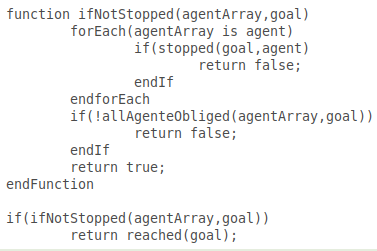
\includegraphics[width=0.6\linewidth]{figure/algrule6.png} 
  \caption{Condição para definir se um dado objetivo foi atingido ou não} \label{wenStop}  
\end{figure}

Se o teste dado por $if(stopped(goaL,agent))$ é verdadeiro para pelo menos um dos agentes, então a função $ifNotStopped(agentArray,goal)$ retorna falso. Se essa situação não acontecer para todos os agentes carregados em $agentArray$, então o algoritmo determina um segundo teste, que é dado pela função $allAgenteObliged(agentArray,goal)$. Essa função verifica se todos os agentes que são obrigados a alcançar o objetivo $goal$ estão contidos em $agentArray$. No contexto desse algoritmo, se a função $allAgenteObliged(agentArray,goal)$ retorna falso, então $ifNotStopped$ também retorna falso, caso contrário $ifNotStopped$ retorna verdade. Se a função $ifNotStopped(agentArray,goal)$ retorna verdade, então o predicado $reached(goal)$ é verdade também. O algoritmo apresenta a função $isTrue$ onde o argumento é o predicado $reached(goal)$. A função $isTrue(arg)$ sempre retorna verdade e tem como por objetivo informar que o seu respectivo argumento é verdade. Isso é necessário tendo em vista a diferença do formalismo adotado pelas demais regras em relação a \ref{wenStop}.

Na linguagem natural essa expressão fica da seguinte forma: se todos os agentes que têm permissão para alcançar um dado objetivo o fizeram sem que esse tenha sido interrompido e considerando que um subgrupo deles é constituído por agentes que são obrigados a isso, então o objetivo é dado como alcançado.

A regra \ref{rolenextgoal} apresenta a condição adequada para quando um agente está habilitado para atingir novos objetivos. Para isso, ele deve possuir um papel onde existe uma permissão para que ele possa atingir o próximo objetivo. Isso é traduzido por $ adoptsRole(ag_n,\rho_m) \wedge hasPermission(\rho_m,g_j) $. Não apenas isso, mas o objetivo atual do agente deve ter sido atingido $ reached(g_i) $ e o objetivo em interesse deve estar associado como predicado $nextGoal(g_i,g_j)$. O termo $enabledToStart(ag_i,g_j)$ corresponde semanticamente apenas que o agente está habilitado a buscar novos objetivos mas não significa que isso implicará em $starts(ag_i,g_j)$ pois o que decide esses processos de transição consiste em aspectos que não correspondem a esse modelo. Essa dinâmica é discutida mais tarde na seção de \textit{Predicados de Controle}.

\begin{eqnarray}\label{rolenextgoal}
	adoptsRole(ag_n,\rho_m) \wedge hasPermission(\rho_m,g_j) \wedge nextGoal(g_i,g_j) \wedge reached(g_i) \nonumber \\
	\to enabledToStart(ag_i,g_j) \nonumber \\
    ag_i, ag_n \in Agent, \rho_m \in Role, g_j \in Goal, g_i \in Goal
\end{eqnarray}

Em linguagem natural, a regra \ref{rolenextgoal} exibe o seguinte: se um agente que alcançou um objetivo atual tem um papel que lhe dá permissão para buscar o próximo objetivo, então esse agente está habilitado para fazer isso.

A regra \ref{rolelastgoal} apresenta a condição de parada do agente em relação ao seu papel, pois se o agente, que tem um determinado papel, cumpriu com todos os objetivos designados a ele, então ele deve encerrar sua operação. A verificação do papel é dado por $adoptsRole(ag_n,\rho_m) \wedge hasPermission(\rho_m,g_i)$, a análise semântica sobre o último objetivo associado a um certo papel é dado por $lastGoal(g_i,\rho_m)$ e a verificação se aquele último objetivo foi atingido é dado por $reached(g_i)$. 

\begin{eqnarray}\label{rolelastgoal}
	adoptsRole(ag_n,\rho_m) \wedge hasPermission(\rho_m,g_i) \wedge lastGoal(g_i,\rho_m) \wedge reached(g_i) \nonumber \\
	\to stopped(g_i) \nonumber \\
    ag_n \in Agent, \rho_m \in Role, g_i \in Goal
\end{eqnarray}

Portanto, a regra \ref{rolelastgoal} em linguagem natural é definida da seguinte maneira: Se um agente cumpriu com todos os objetivos associados a permissão do papel dele, então esse agente deve encerrar suas atividades (em relação a esse papel). 


		\subsection{Diagrama de Atividades} \label{umldiagram}
		
			As Figuras \ref{atividiagram1}, \ref{atividiagram2} e \ref{atividiagram3} (o diagrama foi quebrado em três Figuras distintas com o propósito de melhorar a qualidade da resolução)  apresentam a aplicação das regras em termos de diagrama de atividades. Essas Figuras deve ser entendidas como uma proposta de orientação das regras registradas na subseção \ref{regras}. Há outras maneiras de organizar essas regras em diferentes diagramas de atividades, sendo que a apresentada neste texto é apenas uma dessas. Isso se deve ao fato de que esse estudo pretendo fornecer um modelo e não um algoritmo. 

O primeiro termo desta Figura corresponde a "carregar todos os agentes". Esse elemento é indiferente à estrutura das regras do modelo. A existência desta atividade no diagrama se dá por finalidades de implementação, uma vez que para uma máquina poder processar todos as atividades, primeiramente se faz necessário que informações sobre os agentes sejam carregadas na memória. As atividades "selecione um dos agentes", "carregar os objetivos", "há objetivos que não foram alcançados" e "o agente escolhe por tentar alcançar o objetivo" fazem referência as regras \ref{rolenextgoal} e \ref{reldeonticrole}. Aquela analisa qual é a próxima regra que esta em condições de serem atingidas pelo agente e esta verifica a permissão do agente no que tange a possibilidade de poder adotar o objetivo. 

O ponto de decisão "todas as condições necessárias para esse objetivo estão presentes?" A atividade "violação de condição" fazem referência a regra \ref{conditionViol}, que define uma violação de condição para o caso do agente tentar executar alguma atividade sem que todas as condições estejam presentes naquele instante.

O ponto de decisão "todas as entidades necessárias para esse objetivo estão presentes?" A atividade "violação de relação" fazem referência a regra \ref{entityViol}, pois definem o ocorrido no que diz respeito a ausência de uma entidade ao verificar um dado objetivo em análise. 

\begin{figure}[H]
  \centering
  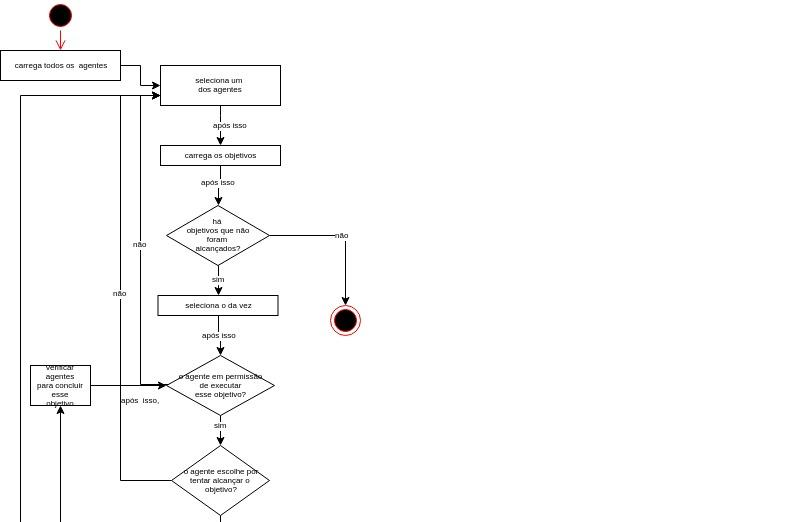
\includegraphics[width=1.1\linewidth]{figure/diag1.jpg} 
  \caption{Diagrama de atividades do modelo (1)}
  \label{atividiagram1}
\end{figure}


\begin{figure}[H]
  \centering
  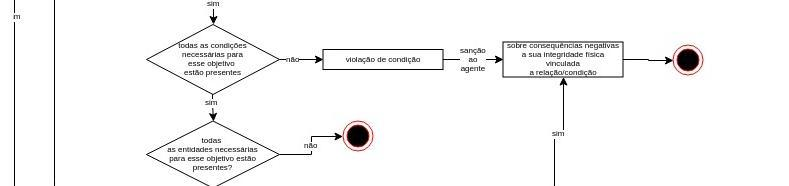
\includegraphics[width=1.1\linewidth]{figure/diag2.jpg} 
  \caption{Diagrama de atividades do modelo (2)}
  \label{atividiagram2}
\end{figure}

\begin{figure}[H]
  \centering
  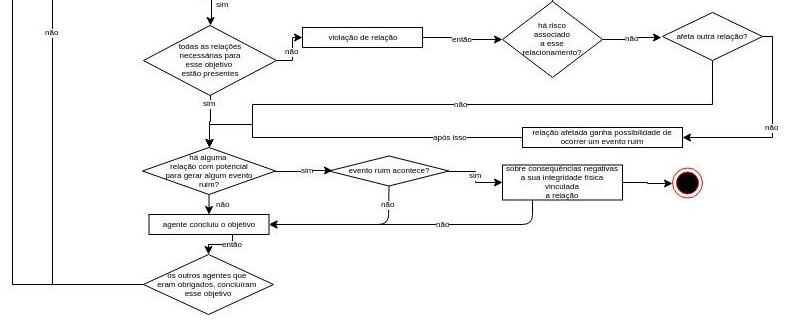
\includegraphics[width=1.1\linewidth]{figure/diag3.jpg} 
  \caption{Diagrama de atividades do modelo (3)}
  \label{atividiagram3}
\end{figure}


O ponto de decisão "todas as relações para esse objetivo estão presentes" e "violação de relação" representam a regra \ref{relationViol}. Isso se deve ao fato de que essas atividades avaliam se uma das relações necessárias para cumprir com o objetivo não está presente, resultando em uma violação de relacionamento. 

As atividades "violação de condição", e "sobre consequências negativas a sua integridade física vinculada a relação/condição" condizem com a regra \ref{consconditionViol} que define as consequências de uma violação de condição. A atividade "violação de relação" em conjunto com a segunda atividade das presentes na sentença anterior fazem referência a regra \ref{consrelationViol}, pois apresenta as sanções relacionadas a uma violação de relacionamento. 

O ponto de decisão "há risco associado a esse relacionamento?", "afeta  outra relação" e "relação afetada ganha possibilidade de ocorrer um evento ruim", apontam para a regra \ref{entityViolaffect} pois ambas situações representam como a ocorrência de uma violação de relacionamento afeta um outro relacionamento. A regra \ref{paybutiamnotguilty} corresponde aos seguintes aspectos do diagrama, "há alguma relação com potencial para gerar algum evento ruim?", "evento ruim acontece?","sobre consequências negativas a sua integridade física vinculadas a relação" tendo em vista a equivalência semântica entre esses elementos sendo que ambas as representações se preocupam com a análise de relações que possuem possibilidades de algum evento ruim surgir sobre o agente do objetivo. 

A regra \ref{consvioent} é representada por "violação de entidade" e pelo elemento que indica o fim do programa. Isso se deve ao fato de que a regra \ref{consvioent} determina o encerramento do processo na ocorrência de uma violação de entidade. 

Os eventos "agente concluiu o objetivo", "os outros agentes que eram obrigados, concluíram esse objetivo" e "verificar agentes para concluir esse objetivo" apontam para as regras \ref{rolenextgoal}, \ref{rolelastgoal}. Esse conjunto de atividades e pontos de decisões apresentam os critérios para definir quando um objetivo foi totalmente alcançado (que é a mesma finalidade dessas regras justificando a equivalência entre ambos formalismos).  A regra \ref{wenStop} é explicitada no diagrama toda vez que a atividade "sobre consequências negativas a integridade física vinculada  a relação/condição" aponta para o fim do programa, tendo em vista que ambras representações definem o encerramento das atividades na ocorrência de feridos. 

O diagrama presente nas Figuras \ref{atividiagram1}, \ref{atividiagram2} e \ref{atividiagram3} apresenta \ref{conditionViol} como a primeira regra de violação a ser executada. O motivo disto reside no fato de que essa regra verifica se o agente respeitou todas as condições do ambiente. Se o agente não fizer isso, ele está sujeito a penalidades físicas encerrando o programa. Ou seja, não abre margens para verificação de outras violações, porque em um caso real, alguém que executa uma atividade sem que todas as condições estejam presentes, então esse alguém está fadado a encerrar qualquer ação em curso. Mesmo que esse alguém estivesse na condição de cometer outras violações, não seria possível fazê-las pois esta primeira violação cometida por ele foi o suficiente para interromper os procedimentos como um todo. Esse mesmo principio fundamenta o sequenciamento das demais regras, sendo que logo em seguida é a \ref{entityViol}, pois se alguma entidade  necessária (ferramenta), não estiver presente no cenário,então não existe possibilidade da continuidade dos procedimentos inviabilizando a realização das relações não fazendo sentido verificar \ref{relationViol}. Contudo, os engenheiros definem essa estrutura apenas como uma proposta que deve ser modificada em função dos interesses da aplicação. Por exemplo, supondo que uma equipe tenha o interesse de usar este modelo para desenvolver jogos sérios com a intenção de analisar todas as violações que podem ser cometidas por um jogador um dado cenário, então para esse caso não há sentido usar esse fluxo de atividades. Em uma condição assim, os engenheiros do jogo devem - usando as mesmas regras - mudar o fluxo do diagrama de atividade para verificar todas as regras de violação antes de analisar se o programa deve ou não ser interrompido.

		\subsection{Predicados Abertos e Fechados} \label{cenarios}
		
			Esse estudo apresenta duas categorias de predicados: \textit{abertos} e \textit{fechados}. Os predicados fechados são aqueles cujo usuário do modelo não possui a liberdade de definir sua
estrutura interna por intermédio de outras regras lógicas ou por valores. Isso se dever ao fato de que esses vocábulos tem sua estrutura alicerçada nas concepções deste modelo sendo que 
são essencias para que o sistema funcione como foi concebido para ser. Assim sendo, o modelador deve fazer uso delas apenas com o propósito de especificar os objetos de interesse. 
Em termos práticos não existe dificuldade em identificar esses predicados, pois sua própria natureza não abre margem para que o modelador consiga escrever novos predicados e novas regras para 
determinar o seu respectivo valor. 

Esses predicados são $thereIsRelation(r_l,e_i,e_k)$, $hasRole(ag_n,\rho_m)$, $hasObligation(\rho_m,g_j)$,
$hasPermission(\rho_m, g_j)$, $isReached(g_k)$, $stopIn(g_n, ag_m)$, $nextGoal(g_i,g_j)$, $hasCondition(g_i,cg_n)$,
$hasEntity(g_i,eg_m)$, $hasRelation(g_i,rg_m)$, $violationCondition(ag_i,g_j,c_k) $, $ violationRelation(ag_i,g_j,r_k) $,
$ violationEntity(ag_i,g_j,e_k) $,  $ hasRisk(X, risk_j, cs_k) $, $possibilityHappensBadEvent(r_l)$, 
$affectsOtherRelations(r_k,r_n)$, $consequenceOfBadEvenet(g_k, ag_i,risk_k,cs_m)$  e $lastGoal(g_i,\rho_m)$. 


Para exemplificar, pode-se considerar o predicado $thereIsRelation(r_l,e_i,e_k)$. Se existir uma entidade $A$,
uma entidade $B$ e uma relação entre $relAB$, então esse termo é escrito desta forma: 
$thereIsRelation(relAB,A,B)$. O valor verdade deste predicado não pode ser modificado para a criação de algum 
cenário e nem pode determinado por outras regras. Se modelador fizer isso então estará modificando a estrutura 
do modelo. Ou seja, esse é um predicado fechado no que tange a aspectos fundamentais aos aspectos semanticos 
desta representação. 

Por outro lados os predicados \textit{abertos} possuem um correspondente sintatico e semântico no modelo mas 
os seus valores devem ser forçados conforme o cenário que se deseja criar ou conforme outras regras de 
implicabilidade. A não determinação destes predicados inviabilizam que o modelo seja analisador de forma 
procedural. Faz parte deste conjunto os seguintes termos: $isPresent(X)$,$tryReach(ag_i,g_j)$ e $happensBadEvent(r_m)$.

Pode-se considerar o seguinte exemplo: Um agente $ag_a$ deve executar o objetivo $g_1$ e $g_2$, os predicados 
a seguir implementam este modelo para o exemplo:

\begin{itemize}
    \item $nextGoal(g_1,g_2)$
    \item $thereIsRelation(rAB,entA,entB)$
    \item $thereIsRelation(rCE,entC,entE)$
    \item $entA \in eg_1 ,entB \in eg_1$
    \item $entC \in eg_2, entD \in eg_2$
    \item $rAB \in rg_1$,
    \item $rCE \in rg_2 $
    \item $cond_1 \in {cg_1} $
    \item $ hasCondition(g_1,cg_1)$
    \item $ hasCondition(g_2,cg_2 )$
    \item $ hasEntity(g_1,eg_1) $
    \item $ hasEntity(g_2,eg_2) $
    \item $ hasRelation(g_1, rg_1 )$
    \item $ hasRelation(g_2, rg_2)$ 
    \item $ affectsOtherRelations(rAB,rCE) $ 
    \item $hasRisk(cg_1,risk_1,cs_1)$
    \item $hasRisk(rCE,risk_2,cs_2)$
    \item $hasRole(ag_a,\rho_1)$
    \item $hasObligation(\rho_1,g_1)$
    \item $hasObligation(\rho_1,g_2)$
\end{itemize}

Apesar de todos os predicados denotarem uma dada condição e de serem o suficientes para definir uma certa 
representação de mundo, não é possível fazer raciocínio algum. Isso, pois não se sabe quais são as ações 
dos agentes e não se sabe quais condições e cenários se deseja representar.  

Para isso, se faz necessário definir um cenário de mundo. Por exemplo, pode-se definir o seguinte cenário; 
$tryReach(ag_a,g_1)$, $\neg isPresent(rAB), tryReach(ag_b,g_2)$ e $ possibilityHappensBadEvent(rCE) \to $  
$happensBadEvent(rCE)$. 

Para esse caso é possível obter as 
seguintes relações de inferência: 

\begin{eqnarray}
	hasRelation(g_1,rg_1)\wedge \neg isPresent(rAB) \wedge (rAB \in rg_1) \wedge tryReach(ag_a,g_1) \to \nonumber \\
	violationRelation(ag_a,g_1,rAB) 
\end{eqnarray}

\begin{eqnarray}
	violationRelation(ag_a,g_1,rAB)  \wedge affectsOtherRelations(rAB,rCE) \nonumber \\
    \to possibilityHappensBadEvent(rCE)  
\end{eqnarray}


\begin{eqnarray}
	possibilityHappensBadEvent(rCE) \to happensBadEvent(rCE) 
\end{eqnarray}



\begin{eqnarray}\label{paybutiamnotguilty}
	possibilityHappensBadEvent(rCE) \wedge  \nonumber \\
    happensBadEvent(rCE) \wedge  \nonumber \\
    hasRelation(g_2,rg_2) \wedge  \nonumber \\
    (rCE \in rg_2) \nonumber \wedge  \nonumber \\
    hasRisk(rCE,risk_2,cs_2) \wedge  \nonumber \\
    tryReach(ag_a,g_2) \nonumber  \nonumber \\
	\to consequenceOfBadEvent(g_2,ag_a,risk_2,cs_2) 
\end{eqnarray}


\begin{eqnarray}\label{badcons}
	consequenceOfBadEvent(g_2,ag_a,risk_2,cs_2) \to stopIn(g_2) 
\end{eqnarray}


Esses racicínios e conclusões só foram possíveis porque o modelador forçou o valor de três predicados e definiu uma relação de implicação. 
Isso acontece por conta de três motivos: 1 - Esse é um modelo de \textit{SMA}, 2 - esse modelo apresenta grau de liberdade para escolher 
a disposição das entidades, condições e relações e 3 - não há como definir a solução de uma possibilidade. 

Para o primeiro caso o predicado $tryReach(ag_i,g_j)$ é resultado de estados internos do agente. Por exemplo, o desenvolvedor pode 
programar um agente que possui o estado de medo, então sobre certas condições ele resolve não tentar alcançar o objetivo gerando 
valor falso para esse predicado, ou pode definir um agente que ponderá pouco ao decidir se deve ou não tentar alcançar um dado objetivo. 
Isso pode ser feito por meio de modelos de agentes tais como: agentes lógicos, arquitetura BDI, 
agentes reativos e agentes em camada. Se for do interesse do modelador, o mesmo pode simplesmente definir o valor verdade para o 
predicado em certas condições. 

O mesmo se aplica para o $isPresent(X)$ onde desenvolvedor pode definir um cenário que, por meio de 
estados internos, os agentes esqueceram uma determinada ferramenta em um certo local ou, por exemplo, que o agente apresenta um 
algoritmo para determinar qual ferramenta é a mais apropriada para uma dada condição. Assim como o moleador é livrer para 
gerar diferentes cenários simplesmente por definir valores diferentes para $isPresent(X)$. Por exemplo, supondo que uma equiple está 
desenvolvendo um jogo sério para avaliar profissionais de uma certa industria. Para avaliar a competencia dos trabalhadores, o 
modelador poderá usar este predicado por adicionar o remover com base nas necessidades de avaliação.

O terceiro motivo reside no fato de que o predicado $possibilityHappensBadEvent(X)$ denota apenas que existe uma possibilidade de ocorrer 
algum determinado evento ruim  $happensBadEvent(X)$. Contudo, se esse evento ocorrerá ou não, não é 
possível definir pois isso depende de questões estatísticas do objeto de estudo. Assim sendo, o usuário deste 
modelo possui algumas possibilidades de ação, tais como: quando $possibilityHappensBadEvent(X)$  for verdade, 
então definir $happensBadEvent(X)$ por meio de um número aleatório, para dadas situações onde ocorre 
$possibilityHappensBadEvent(X)$ tratar $happensBadEvent(X)$ como verdade e para dadas situações 
tratar $happensBadEvent(X)$ como falso ou definir verdade para $happensBadEvent(X)$ como base em algum estudo 
probabilistico. Isso dependerá da finalidade dos modeladores. 


	\section{Caso de Estudo} \label{studycase}


			O estudo de caso desta pesquisa consiste em sete profissionais de linha viva (profissionais que realizam manutenção em equipamentos elétricos energizados) são designados com o propósito de realizar a substituição de um isolador de pedestal. Os papeis desses desses profissionais são; um supervisor e seis executores. A manutenção deve ser executada apenas sobre as seguintes condições: céu ensolarado e umidade relativa do ar menor que 70 porcento. Todos os profissionais devem possuir os EPI's necessários: capacete, óculos de sol, roupa isolante e antichamas, luvas isolantes e botas isolantes. Os profissionais que entram no potencial devem estar vestidos de roupa condutiva e cabo guarda. As ferramentas necessárias para resolver esse problema são: bastão garra de diâmetro 64 x 3600 mm, sela de diâmetro 65, colar, corda de fibra sintética, carretilha, chave com catraca, bastão universal, soquete adequado, locador de pino e bastão com soquete multiangular. O método selecionado para esse tipo de manutenção é a distância onde o eletricista não acessa diretamente o potencial, mas faz isso por intermédio de um bastão isolante. A substituição do isolador 
de pedestal pode ser escrita nos seguintes objetivos: 

\begin{enumerate}
	\item Limpar, secar e testar corda.
	\item Instalar Bastão Garra na estrutura com o pedestal a ser substituído.
	\item Instalar sela com colar na estrutura
	\item Amarrar o bastão na parte superior da estrutura com a corda.
	\item Amarrar o olhal do bastão ao cavalo da sela atrás de uma corda.
	\item Instalar um segundo conjunto bastão e sela no lado oposto da estrutura.
	\item Enforcar um estropo de Náilon no corpo do isolador.
	\item Colocar a extremidade do estropo no gancho da corda de serviço.
	\item Afrouxar os parafusos do conector que prendem a barra ao isolador.
	\item Terminar de retirar os parafusos com o bastão com o soquete multiangular.
	\item Elevar a barra através da corda que une a sela ao bastão.
	\item Apertar o colar através da porca borboleta.
	\item Segurar firmemente a corda de serviço.
	\item Sacar parafusos da base da coluna.
	\item Baixar o isolador ao solo
	\item Içar o Isolador
	\item Colocar Parafusos na base da coluna.
	\item Baixar a barra para que a mesma apoie no novo isolador.
	\item Colocar os parafusos do conector que prende a barra ao novo isolador. 
	\item Retirar Equipamentos
\end{enumerate}

A tabela \ref{agents} apresenta todos os agentes que fazem parte da manutenção. 
\begin{table}[H]
\scalefont{0.8}
\centering
\begin{tabular}{|l|l|}
\hline
\textbf{símbolo} & \textbf{significado} \\ \hline
agente1 & Um dos agentes participantes da manutenção \\ \hline
agente2 & Um dos agentes participantes da manutenção \\ \hline
agente3 & Um dos agentes participantes da manutenção \\ \hline
agente4 & Um dos agentes participantes da manutenção \\ \hline
agente5 & Um dos agentes participantes da manutenção \\ \hline
agente6 & Um dos agentes participantes da manutenção \\ \hline
agente7 & Um dos agentes participantes da manutenção \\ \hline
\end{tabular}
\caption{Os agentes que constituem uma manutenção}
\label{agents}
\end{table}

 A tabela \ref{roles} apresenta todas as funções que deverão ser exercidas pelos agentes.

\begin{table}[H]
\scalefont{0.8}
\centering
\begin{tabular}{|l|l|}
\hline
\textbf{papel} & \textbf{descrição} \\ \hline
supervisor & Atribui papel a outros profissionais \\ \hline
executor1 & Tem como por finalidade executar certas atividades manuais vinculadas a manutenção \\ \hline
executor2 & Tem como por finalidade executar certas atividades manuais vinculadas a manutenção \\ \hline
executor3 & Tem como por finalidade executar certas atividades manuais vinculadas a manutenção \\ \hline
executor4 & Tem como por finalidade executar certas atividades manuais vinculadas a manutenção \\ \hline
executor5 & Tem como por finalidade executar certas atividades manuais vinculadas a manutenção \\ \hline
\end{tabular}
\caption{Os papeis relevantes para a ocorrência da manutenção}
\label{roles}
\end{table}

A tabela \ref{agentsroles} define o predicado $hasRole(ag_n,\rho_m)$ onde $ag_n$ é representado pela coluna agente e $\rho_m$ é representado pela coluna papel.

\begin{table}[H]
\scalefont{0.8}
\centering
\begin{tabular}{|l|l|}
\hline
\textbf{agente} & \textbf{papel} \\ \hline
agente1 & supervisor \\ \hline
agente2 & executor1 \\ \hline
agente3 & executor1 \\ \hline
agente4 & executor2 \\ \hline
agente5 & executor3 \\ \hline
agente6 & executor4 \\ \hline
agente7 & executor5 \\ \hline
\end{tabular}
\caption{Relação $hasRole(ag_n,\rho_m)$}
\label{agentsroles}
\end{table}

A tabela \ref{artefacts} apresenta todos artefatos que fazem parte da descrição deste estudo de caso.

\begin{table}[H]
\scalefont{0.8}
\centering
\begin{tabular}{|l|p{0.8\linewidth}|}
\hline
\textbf{artefato} & \textbf{descrição} \\ \hline
capacete & EPI usado pelo profissional para proteger a cabeça \\ \hline
óculos & Óculos usado para evitar dificuldades de enxergar presentes em dias claros \\ \hline
roupagem & Consiste em roupas isolantes e anti-chamas \\ \hline
luva & Luvas Isolantes \\ \hline
bota & Botas Isolantes para evitar que o profissional seja eletrocutado \\ \hline
bastaoGarra & bastão isolante que possui uma ferramenta em estrutura de garra. 64 X 3600 mm \\ \hline
sela & Possui diâmetro 65 mm, é fixada na torre para sustentar o bastão. \\ \hline
colar & Estrutura que fica fixa na sela, bastão isolante é travado no colar. \\ \hline
corda & Corda Isolante. \\ \hline
carretilha & Carretilha que, em conjunto com a corda, é usada para mover material na vertical. \\ \hline
bastaoUniversal & Bastão isolante que permite o acoplamento de múltiplas ferramentas. \\ \hline
soquete & Usado na manipulação de parafusos. \\ \hline
locador & Usado como pino direcional em alinhamento de furo de parafusos, auxiliado na inserção de pinos e parafusos. \\ \hline
bastaoGarra & Bastão Universal que possui uma garra. \\ \hline
isoladorVelho & Isolador de pedestal danificado a ser substituído \\ \hline
isoladorNovo & Isolador de pedestal novo que será posicionado no local do isolador velho. \\ \hline
torre & Estrutura metálica onde fica fixo o isolador \\ \hline
condutor & Em formato de cabo, fica fixo sobre o topo do isolador.e é por onde passa grandes quantidades de energia elétrica. \\ \hline
estropo & pano firme usado para segurar Isolador quando estiver suspenso \\ \hline
pano & pano usado para limpar ferramentas \\ \hline
glicerina & substância usada para limpar as ferramentas adequadamente \\ \hline
condutímetro & Medidor de corrente de fuga sobre o bastão universal. \\ \hline
parafuso & Parafusos prendem o conector condutor-Isolador e também prendem o Isolador a base \\ \hline
conector & Estrutura que tem como por finalidade manter condutor,cabeçote do isolador em conjunto. \\ \hline
\end{tabular}
\caption{Definindo todos os artefatos presentes na manutenção}
\label{artefacts}
\end{table} 

As etapas da atividade anteriormente postas foram analisadas em conjunto com engenheiros da área e foram estruturadas com base nos objetivos expostos na tabela \ref{g}. Essa tabela também apresenta as especificações para o predicado $nextGoal(g_i,g_j)$ onde \textit{Objetivo} representa $g_i$, \textit{Próximo} $g_j$ e \textit{Descrição} é referente a $g_i$.

\begin{table}[H]
\scalefont{0.8}
\centering
\begin{tabular}{|l|l|p{0.6\linewidth}|}
\hline
\textbf{Objetivo} & \textbf{Próximo} & \textbf{Descrição} \\ \hline
gSupervisor & g1,g6 & Atribui objetivos aos demais agentes. \\ \hline
g0 &  gSupervisor & Vestir os AP'Is \\ \hline
g1 &  g2 & Limpar, secar e testar ferramentas com material isolante. \\ \hline
g2 &  g3 & Medir a corrente de fuga de ferramentas isolantes \\ \hline
g3 &  g4 & Instalar sela com colar na estrutura \\ \hline
g4 &  g5 & Passar o bastão garra por dentro do olhal do colar. \\ \hline
g5 &  g12 & Amarrar o bastão garra na parte superior da estrutura com a corda, fixar no condutor \\ \hline
g6 &  g7 & Amarrar o olhal do bastão garra ao cavalo da sela atrás de uma corda. \\ \hline
g7 &  g8 & Instalar sela com colar no outro lado da estrutura estrutura \\ \hline
g8 &  g9 & Passar o bastão universal por dentro do olhal do colar \\ \hline
g10 & g11 & Pender carretilha no bastão Universal. \\ \hline
g11 & g12 & Amarrar o bastão universal na parte superior da estrutura com a corda; \\ \hline
g12 & g13 & Rotacionar estrutura olhal garra em 45 graus. \\ \hline
g13 & g14 & Enforcar um estropo de Náilon no corpo do isolador velho. \\ \hline
g14 & g15 & Colocar a extremidade do estropo no gancho da corda de serviço. \\ \hline
g15 & g16 & Afrouxar os parafusos do conector que prendem a barra ao isolador. \\ \hline
g16 & g17 & Terminar de retirar os parafusos com o bastão com o soquete multiangular. \\ \hline
g17 & g18 & Elevar o condutor através da corda que une a sela ao bastão. \\ \hline
g18 & g19 & Apertar o colar através da porca borboleta. \\ \hline
g19 & g20 & Sacar parafusos da base da coluna. \\ \hline
g20 & g21 & Segurar firmemente a corda de serviço,baixar o isolador ao solo \\ \hline
g21 & g22 & Passar Estropo no Isolador Novo \\ \hline
g22 & g23 & Colocar a extremidade do estropo no gancho da corda de serviço. \\ \hline
g23 & g24 & Içar o Isolador \\ \hline
g24 & g25 & Colocar Parafusos na base da coluna. \\ \hline
g25 & g26 & Baixar o condutor para que a mesma se sustente no novo isolador. \\ \hline
g26 & g27 & Colocar os parafusos do conector que prende a barra ao novo isolador. \\ \hline
g27 &     & Retirar Equipamentos \\ \hline
\end{tabular}
\caption{Define e descreve os objetivos bem como os respectivos pré-requisitos}
\label{g}
\end{table}

A tabela \ref{condition} apresenta $c_k$ dado pela coluna condição e pela coluna descrição. Essa tabela define $hasRisk(c_k,risk_j,cs_m)$ onde $risk_j$ é descrito pela coluna risco e $cs_m$ é descrito como consequência. 

\begin{table}[H]
\scalefont{0.8}
\centering
\begin{tabular}{|l|p{0.6\linewidth}|l|l|}
\hline
\textbf{condição} & \textbf{descrição} & \textbf{risco} & \textbf{consequência} \\ \hline
umidade70 & Umidade Relativa do Ar deve ser inferior a setenta porcento. & eletrocutado & morte \\ \hline
noVento & Não deve haver vento durante os procedimentos de manutenção. & eletrocutado & morte \\ \hline
noChuva & Não deve haver chuva durante o ato da manutenção & eletrocutado & morte \\ \hline
sol & O dia deve estar ensolarado & eletrocutado & morte \\ \hline
\end{tabular}
\caption{Define as condições necessárias para que a manutenção tenha possibilidade de acontecer}
\label{condition}
\end{table}


As tabelas \ref{relationEntEnt1}, \ref{relationEntEnt2} apresentam a especificação para dois predicados onde uma deles é $thereIsRelation(r_l,e_i,e_k)$ 
tal que $r_l$ é definido pela coluna \textit{relacionamento}, $e_i$ e $e_k$ pelas \textit{entidades envolvidas}. 
O outro predicado é dado por $hasRisk(r_k,risk_j,cs_m)$ onde $risk_j$ é dado pela coluna risco e $cs_m$ é dado pela coluna $consequencia$. 
Algumas relações (instâncias do conjunto $Relation$) serão apresentadas usando o termo $X$. O objetivo disto consiste tornar as tabelas mais enxutas por intermédio de uma regra a qual é;
A variável $X$ deve ser substituída pelo agente que tem a permissão de executar alguma ação em dado objetivo em prol a sua função. 
Essa regra pode ser sintetizada na seguinte expressão para um agente $ag_n$ que é referenciado por $AGENT$:

\begin{eqnarray}\label{whenusex} \nonumber
    hasRole(AGENT,\rho_m) \wedge hasPermission(\rho_m,g_i) \wedge (relXotherEntity \in rg_n)  \\ 
    \wedge hasRelation(g_i,rg_n) \to relAGENTotherEntity 
\end{eqnarray}


Para mostrar como se dá o uso desta regra pode-se considerar um relacionamento $ relXCapacete$ entre $X$ e $capacete$ (essa relação será melhor descrita nas tabelas \ref{relationEntEnt1}, \ref{relationEntEnt2}). Essa relação acontece no objetivo $g_0$ onde o trabalhador deve colocar o capacete em sua cabeça, por conta disto se aplica a todos os agentes que representam esses profissionais. Nesta implementação, esses agentes são: $agente1$, $agente2$, $agente3$, $agente4$, $agente5$, $agente6$ e $agente7$. Aplicando a regra \ref{whenusex} para esse caso, obtêm-se as seguintes relações: $relAgente1Capacete$, $relAgente2Capacete$, $relAgente3Capacete$, $relAgente4Capacete$, $relAgente5Capacete$, $relAgente6Capacete$ e $relAgente7Capacete$. Portanto, nas tabelas \ref{relationEntEnt1}, \ref{relationEntEnt2}, ao ler:  

\begin{eqnarray}
	relXCapacete | X,capacete |
\end{eqnarray}

Para o objetivo $g_0$, essa linha é equivalente a: 

\begin{eqnarray}
relAgente1Capacete | Agente1 ,capacete | \nonumber \\
relAgente2Capacete | Agente2 ,capacete | \nonumber \\ 
relAgente3Capacete | Agente3 ,capacete | \nonumber \\ 
relAgente4Capacete | Agente4 ,capacete | \nonumber \\
relAgente5Capacete | Agente5 ,capacete | \nonumber \\
relAgente6Capacete | Agente6 ,capacete | \nonumber \\
relAgente7Capacete | Agente7 ,capacete | \nonumber \\
\nonumber \\
\end{eqnarray}

\begin{table}[H]
\centering
\scalefont{0.6}
\begin{tabular}{|l|l|l|l|}
\hline
\textbf{relacionamento}                  & \textbf{entidades envolvidas}                & \textbf{risco}                & \textbf{consequência}              \\ \hline
relXCapacete                             & X,capacete                                     & nenhum                          & nenhum                               \\ \hline
relXOculos                               & X,oculos                                       & nenhum                          & nenhum                               \\ \hline
relXRoupagem                             & X,roupagem                                     & nenhum                          & nenhum                               \\ \hline
relXLuva                                 & X,luva                                         & nenhum                          & nenhum                               \\ \hline
relXBotas                                & X,bota                                         & nenhum                          & nenhum                               \\ \hline
relXPano                                 & X,pano                                         & nenhum                          & nenhum                               \\ \hline
relPanoGlicerina                         & pano,glicerina                                 & nenhum                          & nenhum                               \\ \hline
relPanoCorda                             & pano,corda                                     & nenhum                          & nenhum                               \\ \hline
relPanoBastoaUniversal                   & pano,bastaoUniversal                           & nenhum                          & nenhum                               \\ \hline
relPanoSoquete                           & pano,soquete                                   & nenhum                          & nenhum                               \\ \hline
\end{tabular}
\caption{Descrição das entidades em função das relações}
\label{relationEntEnt1}
\end{table}


\begin{table}[H]
\centering
\scalefont{0.6}
\begin{tabular}{|l|l|l|l|}
\hline
\textbf{relacionamento}                  & \textbf{entidades envolvidas}                  & \textbf{risco}                  & \textbf{consequência}              \\ \hline
relPanoBastaoUniversal                   & pano,bastaoGarra                               & nenhum                          & nenhum                               \\ \hline
relXSela                                 & X,sela                                         & nenhum                          & nenhum                               \\ \hline
relXColar                                & X,colar                                        & nenhum                          & nenhum                               \\ \hline
relXBastaoGarra                          & X,bastaoGarra                                  & nenhum                          & nenhum                               \\ \hline
relTorreSela                             & torre,sela                                     & nenhum                          & nenhum                               \\ \hline
relSelaColar                             & sela,colar                                     & nenhum                          & nenhum                               \\ \hline
relColarBastaoGarra                      & colar,bastaoGarra                              & nenhum                          & nenhum                               \\ \hline
relBastaoGarraCondutor                   & bastaoGarra,condutor                           & eletrocutado                    & morte                                \\ \hline
relXBastaoUniversal                      & X,bastaoUniversal                              & nenhum                          & nenhum                               \\ \hline
relCordaBastaoUniversal                  & corda,bastaoUniversal                          & nenhum                          & nenhum                               \\ \hline
relCordaCarretilha                       & corda,carretilha                               & nenhum                          & nenhum                               \\ \hline
relBastaoUniversalCarretilha             & bastaoUniversal,carretilha                     & nenhum                          & nenhum                               \\ \hline
relBastaoUniversalColar                  & bastaoUniversal,colar                          & nenhum                          & nenhum                               \\ \hline
relBastaoUniversalEstopo                 & bastaoUniversal,estopo                         & nenhum                          & nenhum                               \\ \hline
relCordaEstropo                          & corda,estropo                                  & eletrocutado                    & morte                                \\ \hline
relEstropoIsoladorVelho                  & estropo,isoladorVelho                          & nenhum                          & nenhum                               \\ \hline
relXChaveCatraca                         & X,chaveCatraca                                 & nenhum                          & nenhum                               \\ \hline
relChaveCatracaBastaoUniversal           & chaveCatraca,bastaoUniversal                   & nenhum                          & nenhum                               \\ \hline
relChaveCatracaParafuso                  & chaveCatraca,parafuso                          & eletrocutado                    & morte                                \\ \hline
relParafusoConector                      & parafuso,conector                              & eletrocutado                    & morte                                \\ \hline
relXBastaoSoquete                        & X,bastaoSoquete                                & nenhum                          & nenhum                               \\ \hline
relSoqueteParafuso                       & soquete,parafuso                               & eletrocutado			        & morte                                \\ \hline
relXCorda                                & X,corda                                        & eletrocutado                    & morte                                \\ \hline
relXIsoladorVelho                        & X,isoladorVelho                                & nenhum                          & nenhum                               \\ \hline
relXIsoladorNovo                         & X,isoladorNovo                                 & nenhum                          & nenhum                               \\ \hline
relCordaBastaoGarra                      & corda,bastaoGarra                              & nenhum                          & nenhum                               \\ \hline
relBastaoGarraSela                       & bastaoGarra, sela                              & nenhum                          & nenhum                               \\ \hline
relXCarretilha                           & X,carretilha                                   & nenhum                          & nenhum                               \\ \hline
relBastaoUniversalCorda                  & bastaoUniversal,corda                          & nenhum                          & nenhum                               \\ \hline
relBastaoUniversalTorre                  & bastaoUniversal,torre                          & nenhum                          & nenhum                               \\ \hline
relEstropoCorda                          & estropo,corda                                  & eletrocutado                    & morte                                \\ \hline
relEstropoIsoladorNovo                   & estropo,isoladorNovo                           & nenhum                          & nenhum                               \\ \hline
relBastaoUniversalSela                   & universal,sela                                 & nenhum                          & nenhum                               \\ \hline
relBastaoGarraTorre                      & bastaoGarra,torre                              & nenhum                          & nenhum                               \\ \hline
relBastaoUniversalEstropo                & bastaoUniversal,estropo                        & nenhum                          & nenhum                               \\ \hline
relXColar                                & X,colar                                        & nenhum                          & nenhum                               \\ \hline
relParafusoTorre                         & parafuso,torre                                 & eletrocutado                    & morte                                \\ \hline
relCondutivimetroCorda                   & condutímetro,corda                             & nenhum                          & nenhum                               \\ \hline
relCondutivimetroBastaoUniversal         & condutímetro,bastaoUniversal                   & nenhum                          & nenhum                               \\ \hline
relCondutivimetroBastaoGarra             & condutímetro,bastaoGarra                       & nenhum                          & nenhum                               \\ \hline
relCondutivimetroSoquete                 & condutímetro,soquete                           & nenhum                          & nenhum                               \\ \hline
\end{tabular}
\caption{Descrição das entidades em função das relações}
\label{relationEntEnt2}
\end{table}

As tabelas \ref{relation1},\ref{relation2} e \ref{relation3} apresentam a relação $affectsOtherRelations(r_k,r_n)$ onde $r_k$ é representado pela coluna relacionamento-errado e $r_n$ é representado 
pela coluna relacionamento-afetado. 

\begin{table}[H]
\centering
\scalefont{0.6}
\begin{tabular}{|l|l|}
\hline
\textbf{relacionamento-errado} & \textbf{relacionamento-afetado}   \\ \hline
relXCapacete                                    & relBastaoGarraCondutor                           \\ \hline
relXCapacete                                    & relCordaEstropo                                  \\ \hline
relXCapacete                                    & relChaveCatracaParafuso                          \\ \hline
relXCapacete                                    & relParafusoConector                              \\ \hline
relXCapacete                                    & relSoqueteParafuso                               \\ \hline
relXCapacete                                    & relXCorda                                        \\ \hline
relXCapacete                                    & relEstropoCorda                                  \\ \hline
relXOculos                                      & relBastaoGarraCondutor                           \\ \hline
relXOculos                                      & relCordaEstropo                                  \\ \hline
relXOculos                                      & relChaveCatracaParafuso                          \\ \hline
relXOculos                                      & relParafusoConector                              \\ \hline
relXOculos                                      & relSoqueteParafuso                               \\ \hline
relXOculos                                      & relXCorda                                        \\ \hline
relXOculos                                      & relEstropoCorda                                  \\ \hline
relXLuva                                        & relBastaoGarraCondutor                           \\ \hline
relXLuva                                        & relCordaEstropo                                  \\ \hline
relXLuva                                        & relChaveCatracaParafuso                          \\ \hline
relXLuva                                        & relParafusoConector                              \\ \hline
relXLuva                                        & relSoqueteParafuso                               \\ \hline
relXLuva                                        & relXCorda                                        \\ \hline
relXLuva                                        & relEstropoCorda                                  \\ \hline
relXBotas                                       & relBastaoGarraCondutor                           \\ \hline
relXBotas                                       & relCordaEstropo                                  \\ \hline
relXBotas                                       & relChaveCatracaParafuso                          \\ \hline
relXBotas                                       & relParafusoConector                              \\ \hline
relXBotas                                       & relSoqueteParafuso                               \\ \hline
relXBotas                                       & relXCorda                                        \\ \hline
relXBotas                                       & relEstropoCorda                                  \\ \hline
relXPano                                        & relBastaoGarraCondutor                           \\ \hline
\end{tabular}
\caption{Define o impacto que o erro em um relacionamento gera em outro relacionamento}
\label{relation1}
\end{table}

\begin{table}[H]
\centering
\scalefont{0.6}
\begin{tabular}{|l|l|l|}
\hline
\textbf{relacionamento-errado}                  & \textbf{relacionamento-afetado}                  \\ \hline
relXPano                                        & relCordaEstropo                                  \\ \hline
relXPano                                        & relChaveCatracaParafuso                          \\ \hline
relXPano                                        & relParafusoConector                              \\ \hline
relXPano                                        & relSoqueteParafuso                               \\ \hline
relXPano                                        & relXCorda                                        \\ \hline
relXPano                                        & relEstropoCorda                                  \\ \hline
relPanoGlicerina                                & relBastaoGarraCondutor                           \\ \hline
relPanoGlicerina                                & relCordaEstropo                                  \\ \hline
relPanoGlicerina                                & relChaveCatracaParafuso                          \\ \hline
relPanoGlicerina                                & relParafusoConector                              \\ \hline
relPanoGlicerina                                & relSoqueteParafuso                               \\ \hline
relPanoGlicerina                                & relXCorda                                        \\ \hline
relPanoGlicerina                                & relEstropoCorda                                  \\ \hline
relPanoCorda                                    & relCordaEstropo                                  \\ \hline
relPanoCorda                                    & relXCorda                                        \\ \hline
relPanoCorda                                    & relEstropoCorda                                  \\ \hline
relPanoBastaoUniversal                          & relBastaoGarraCondutor                           \\ \hline
relPanoBastaoUniversal                          & relChaveCatracaParafuso                          \\ \hline
relPanoBastaoUniversal                          & relParafusoConector                              \\ \hline
relPanoBastaoUniversal                          & relBastaoGarraCondutor                           \\ \hline
relPanoSoquete                                  & relBastaoGarraCondutor                           \\ \hline
relPanoSoquete                                  & relCordaEstropo                                  \\ \hline
relPanoSoquete                                  & relChaveCatracaParafuso                          \\ \hline
relPanoSoquete                                  & relParafusoConector                              \\ \hline
relPanoSoquete                                  & relSoqueteParafuso                               \\ \hline
relPanoSoquete                                  & relXCorda                                        \\ \hline
relPanoSoquete                                  & relEstropoCorda                                  \\ \hline
relCondutivimetroCorda                          & relBastaoGarraCondutor                           \\ \hline
\end{tabular}
\caption{Define o impacto que o erro em um relacionamento gera em outro relacionamento}
\label{relation2}
\end{table}

\begin{table}[H]
\centering
\scalefont{0.6}
\begin{tabular}{|l|l|l|}
\hline
\textbf{relacionamento-errado}                  & \textbf{relacionamento-afetado}                   \\ \hline
relCondutivimetroCorda                          & relCordaEstropo                                  \\ \hline
relCondutivimetroCorda                          & relChaveCatracaParafuso                          \\ \hline
relCondutivimetroCorda                          & relParafusoConector                              \\ \hline
relCondutivimetroCorda                          & relSoqueteParafuso                               \\ \hline
relCondutivimetroCorda                          & relXCorda                                        \\ \hline
relCondutivimetroCorda                          & relEstropoCorda                                  \\ \hline
relCondutivimetroCorda                          & relParafusoTorre                                 \\ \hline
relPanoBastaoUniversal                          & relBastaoGarraCondutor                           \\ \hline
relPanoBastaoUniversal                          & relChaveCatracaParafuso                          \\ \hline
relPanoBastaoUniversal                          & relParafusoConector                              \\ \hline
relPanoBastaoUniversal                          & relParafusoTorre                                 \\ \hline
relPanoBastaoUniversal                          & relBastaoGarraCondutor                           \\ \hline
relPanoSoquete                                  & relBastaoGarraCondutor                           \\ \hline
relPanoSoquete                                  & relCordaEstropo                                  \\ \hline
relPanoSoquete                                  & relChaveCatracaParafuso                          \\ \hline
relPanoSoquete                                  & relParafusoConector                              \\ \hline
relPanoSoquete                                  & relSoqueteParafuso                               \\ \hline
relPanoSoquete                                  & relXCorda                                        \\ \hline
relPanoSoquete                                  & relEstropoCorda                                  \\ \hline
relPanoSoquete                                  & relParafusoTorre                                 \\ \hline
relCondutivimetroCorda                          & relBastaoGarraCondutor                           \\ \hline
relCondutivimetroCorda                          & relCordaEstropo                                  \\ \hline
relCondutivimetroCorda                          & relChaveCatracaParafuso                          \\ \hline
relCondutivimetroCorda                          & relParafusoConector                              \\ \hline
relCondutivimetroCorda                          & relSoqueteParafuso                               \\ \hline
relCondutivimetroCorda                          & relXCorda                                        \\ \hline
relCondutivimetroCorda                          & relEstropoCorda                                  \\ \hline
relCondutivimetroCorda                          & relParafusoTorre                                 \\ \hline
\end{tabular}
\caption{Define o impacto que o erro em um relacionamento gera em outro relacionamento por mudar a possibilidade de algo errado acontecer.}
\label{relation3}
\end{table}


As tabelas \ref{deontic1}, \ref{deontic2}, \ref{deontic3} e \ref{deontic4},  apresentam a relação $hasObligation(\rho_m,g_i)$ onde $\rho_m$ é representado pela coluna papel e $g_i$ é representado pela coluna objetivo. 

\begin{table}[H]
\centering
\scalefont{0.8}
\begin{tabular}{|l|l|}
\hline
\textbf{papel} & \textbf{objetivo} \\ \hline
executor1 & g0 \\ \hline
executor2 & g0 \\ \hline
executor3 & g0 \\ \hline
executor4 & g0 \\ \hline
executor5 & g0 \\ \hline
supervisor & g0 \\ \hline
supervisor & gSupervisor \\ \hline
executor1 & g1 \\ \hline
executor2 & g1 \\ \hline
executor1 & g2 \\ \hline
executor2 & g2 \\ \hline
executor1 & g3 \\ \hline
executor2 & g2 \\ \hline
executor1 & g4 \\ \hline
executor2 & g4 \\ \hline
executor1 & g5 \\ \hline
executor2 & g5 \\ \hline
executor3 & g6 \\ \hline
executor4 & g6 \\ \hline
executor5 & g6 \\ \hline
executor3 & g7 \\ \hline
executor4 & g7 \\ \hline
executor5 & g7 \\ \hline
executor3 & g8 \\ \hline
executor4 & g8 \\ \hline
executor5 & g8 \\ \hline
executor3 & g9 \\ \hline
executor4 & g9 \\ \hline
executor5 & g9 \\ \hline
\end{tabular}
\caption{Objetivos que devem ser atingidos pelo agente que assumir um dada função}
\label{deontic1}
\end{table}

\begin{table}[H]
\centering
\scalefont{0.8}
\begin{tabular}{|l|l|}
\hline
\textbf{papel} & \textbf{objetivo} \\ \hline
executor3 & g10 \\ \hline
executor4 & g10 \\ \hline
executor5 & g10 \\ \hline
executor3 & g11 \\ \hline
executor4 & g11 \\ \hline
executor5 & g11 \\ \hline
executor1 & g12 \\ \hline
executor2 & g12 \\ \hline
executor3 & g12 \\ \hline
executor4 & g12 \\ \hline
executor1 & g13 \\ \hline
executor2 & g13 \\ \hline
executor3 & g13 \\ \hline
executor4 & g13 \\ \hline
executor1 & g14 \\ \hline
executor2 & g14 \\ \hline
executor3 & g14 \\ \hline
executor4 & g14 \\ \hline
executor2 & g15 \\ \hline
executor3 & g15 \\ \hline
executor4 & g15 \\ \hline
executor5 & g15 \\ \hline
executor2 & g16 \\ \hline
executor3 & g16 \\ \hline
executor4 & g16 \\ \hline
executor5 & g16 \\ \hline
executor1 & g17 \\ \hline
\end{tabular}
\caption{Objetivos que devem ser atingidos pelo agente que assumir um dada função}
\label{deontic2}
\end{table}


\begin{table}[H]
\centering
\scalefont{0.8}
\begin{tabular}{|l|l|}
\hline
\textbf{role} & \textbf{g} \\ \hline
executor3 & g17 \\ \hline
executor4 & g17 \\ \hline
executor5 & g17 \\ \hline
executor1 & g18 \\ \hline
executor3 & g18 \\ \hline
executor4 & g18 \\ \hline
executor5 & g18 \\ \hline
executor1 & g19 \\ \hline
executor3 & g19 \\ \hline
executor4 & g19 \\ \hline
executor5 & g19 \\ \hline
executor1 & g20 \\ \hline
executor3 & g20 \\ \hline
executor4 & g20 \\ \hline
executor5 & g20 \\ \hline
executor1 & g21 \\ \hline
executor3 & g21 \\ \hline
executor4 & g21 \\ \hline
executor5 & g21 \\ \hline
executor1 & g22 \\ \hline
executor2 & g22 \\ \hline
executor3 & g22 \\ \hline
executor5 & g22 \\ \hline
executor1 & g23 \\ \hline
executor2 & g23 \\ \hline
executor3 & g23 \\ \hline
\end{tabular}
\caption{Objetivos que devem ser atingidos pelo agente que assumir um dada função}
\label{deontic3}
\end{table}

\begin{table}[H]
\centering
\scalefont{0.8}
\begin{tabular}{|l|l|}
\hline
\textbf{role} & \textbf{g} \\ \hline
executor5 & g23 \\ \hline
executor1 & g24 \\ \hline
executor2 & g24 \\ \hline
executor3 & g24 \\ \hline
executor5 & g24 \\ \hline
executor1 & g25 \\ \hline
executor2 & g25 \\ \hline
executor3 & g25 \\ \hline
executor4 & g25 \\ \hline
executor1 & g26 \\ \hline
executor2 & g26 \\ \hline
executor3 & g26 \\ \hline
executor4 & g26 \\ \hline
executor1 & g27 \\ \hline
executor2 & g27 \\ \hline
executor3 & g27 \\ \hline
executor4 & g27 \\ \hline
executor5 & g27 \\ \hline
\end{tabular}
\caption{Objetivos que devem ser atingidos pelo agente que assumir um dada função}
\label{deontic4}
\end{table}

A tabela \ref{entities} apresenta as entidades que constituem os conjuntos \textbf{eg}.

\begin{table}[H]
\centering
\scalefont{0.8}
\begin{tabular}{|l|l|}
\hline
\textbf{entidades}                                                                                                    & \textbf{eg} \\ \hline
capacete,óculos,roupagem,luvas,botas X = \{agentes em relação aos objetivos\}                                      & eg0         \\ \hline
pano,glicerina,carretilha,bastaoUniversal,corda,bastaoGarra,X = \{agentes em relação aos objetivos\}               & eg1         \\ \hline
pano,glicerina,carretilha,bastaoUniversal,corda,bastaoGarra,condutímetro,X = \{agentes em relação aos objetivos\}  & eg2         \\ \hline
sela,colarX = \{agentes em relação aos objetivos\}                                                                 & eg3         \\ \hline
colar,bastaoGarraX = \{agentes em relação aos objetivos\}                                                          & eg4         \\ \hline
corda,bastaoGarra,bastaoGarraTorre,condutorX = \{agentes em relação aos objetivos\}                                & eg5         \\ \hline
bastaoGarra,selaX = \{agentes em relação aos objetivos\}                                                           & eg6         \\ \hline
sela,colarX = \{agentes em relação aos objetivos\}                                                                 & eg7         \\ \hline
sela,bastaoUniversal,Colar,X = \{agentes em relação aos objetivos\}                                                & eg8         \\ \hline
bastaoUniversal,carretilha,X = \{agentes em relação aos objetivos\}                                                & eg9         \\ \hline
corda,bastaoUniversal,corda,torre,X = \{agentes em relação aos objetivos\}                                         & eg10        \\ \hline
bastaoUniversal,corda,colar,selaX = \{agente que tenta alcançar o objetivo\}                                       & eg11        \\ \hline
colar,X = \{agentes em relação aos objetivos\}                                                                     & eg12        \\ \hline
bastaoUniversal,estropo,isoladorVelhoX = \{agentes em relação aos objetivos\}                                      & eg13        \\ \hline
bastaoUniversal,corda,estropoX = \{agentes em relação aos objetivos\}                                              & eg14        \\ \hline
chaveCatraca,bastaoUniversal,prafusoX = \{agentes em relação aos objetivos\}                                       & eg15        \\ \hline
bastaoSoquete,parafuso,X = \{agentes em relação aos objetivos\}                                                    & eg16        \\ \hline
bastaoGarra,condutorcordaX = \{agentes em relação aos objetivos\},                                                 & eg17        \\ \hline
colar,X = \{agentes em relação aos objetivos\},                                                                    & eg18        \\ \hline
chaveCatraca,bastaoUniversal,prafusobastaoSoquete,parafuso,torreX = \{agentes em relação aos objetivos\}           & eg19        \\ \hline
cordaX = \{agentes em relação aos objetivos\}                                                                      & eg20        \\ \hline
estropo, isoladorNovo,X = \{agentes em relação aos objetivos\}                                                     & eg21        \\ \hline
bastaoUniversal,corda,estropoX = \{agentes em relação aos objetivos\}                                              & eg22        \\ \hline
cordaX = \{agentes em relação aos objetivos\}                                                                      & eg23        \\ \hline
chaveCatraca,bastaoUniversal,prafusobastaoSoquete,parafuso,torreX = \{agentes em relação aos objetivos\}           & eg24        \\ \hline
bastaoGarra,condutorcordaX = \{agentes em relação aos objetivos\},                                                 & eg25        \\ \hline
chaveCatraca,bastaoUniversal,prafusoX = \{agentes em relação aos objetivos\}                                       & eg26        \\ \hline
sela,colar,bastaoGarra,bastaoUniversal,bastaoSoquete,corda,carretilha,chaveCatraca,torre,condutor                  & eg27        \\ \hline
\end{tabular}
\caption{Entidades que formam os conjuntos $eg_n$. Cada conjunto destes estão relacionados com um objetivo e determinam as entidades necessárias para que o mesmo tenha codição de ser alcançado.}
\label{entities}
\end{table}


As tabelas \ref{relationsgroup1},\ref{relationsgroup2} apresentam as relações que constituem os conjuntos \textbf{rg}.
\begin{table}[H]
\centering
\scalefont{0.7}
\begin{tabular}{|p{0.8\linewidth}|l|}
\hline
\textbf{relacionamentos}                                                                                                                                                                                                                                                                                                                  & \textbf{rg} \\ \hline
relXcapacete relXoculos relXroupagem relXluva relXbotas                                                                                                                                                                                                                                                                                   & rg0         \\ \hline
relXPano relPanoGlicerina relPanoCorda relPanoBastaoUniversal relPanoBastaoGarra relPanoSoquete                                                                                                                                                                                                                                           & rg1         \\ \hline
relCondutivimetroCorda relCondutivimetroBastaoUniversal relCondutivimetroBastaoGarra relCondutivimetroSoquete                                                                                                                                                                                                                                & rg2         \\ \hline
relCondutivimetro                                                                                                                                                                                                                                                                                                                         & rg3         \\ \hline
relXBastaoGarra relColarBastaoGarra                                                                                                                                                                                                                                                                                                      & rg4         \\ \hline
relXBastaoGarra relXCordarelCordaBastaoGarra relBastaoGarraTorre relBastaoGarraCondutor                                                                                                                                                                                                                                                    & rg5         \\ \hline
relBastaoGarraSela relXBastaoGarra relXSela                                                                                                                                                                                                                                                                                               & rg6         \\ \hline
relXSela relXColar relTorreSela                                                                                                                                                                                                                                                                                                           & rg7         \\ \hline
relBastaoUniversalColar relXBastaoUniversal                                                                                                                                                                                                                                                                                              & rg8         \\ \hline
relXBastaoUniversal relXCarretilha relBastaoUniversalCarretilha                                                                                                                                                                                                                                                                           & rg9         \\ \hline
relXCorda relXBastaoUniversal relBastaoUniversalCorda relBastaoUniversalTorre                                                                                                                                                                                                                                                             & rg10        \\ \hline
relXCorda relXBastaoUniversal relXColar relBastaoUniversalColar relBastaoUniversalSela                                                                                                                                                                                                                                                    & rg11        \\ \hline
relXColar                                                                                                                                                                                                                                                                                                                                 & rg12        \\ \hline
relXBastaoUniversal relBastaoUniversalEstropo relEstropoIsoladorVelho                                                                                                                                                                                                                                                                     & rg13        \\ \hline
relXBastaoUniversal relBastaoUniversalCordarelCordaEstropo relEstropoCorda                                                                                                                                                                                                                                                                & rg14        \\ \hline
relChaveCatracaBastaoUniversal relXChaveCatraca relXBastaoUniversal relChaveCatracaParafuso                                                                                                                                                                                                                                               & rg15        \\ \hline
relXBastaoSoquete relSoqueteParafuso                                                                                                                                                                                                                                                                                                      & rg16        \\ \hline
relXCorda relCordaBastaoGarra relBastaoGarraCondutor                                                                                                                                                                                                                                                                                      & rg17        \\ \hline
relXColar                                                                                                                                                                                                                                                                                                                                 & rg18        \\ \hline
relChaveCatracaBastaoUniversal relXChaveCatraca relXBastaoUniversal relChaveCatracaParafuso relParafusoTorre relXBastaoSoquete relSoqueteParafuso                                                                                                     & rg19        \\ \hline
relXCorda                                                                                                                                                                                                                                                                                                                                 & rg20        \\ \hline
relXEstropo relEstropoIsoladorNovo                                                                                                                                                                                                                                                                                                        & rg21        \\ \hline
relXBastaoUniversal relBastaoUniversalCorda relCordaEstropo relEstropoCorda                                                                                                                                                                                                                                                               & rg22        \\ \hline
relXCorda                                                                                                                                                                                                                                                                                                                                 & rg23        \\ \hline
\end{tabular}
\caption{Relacionamentos que formam os conjuntos $rg_n$. Cada conjunto $rg_n$ está relacionado com um objetivo A relação entre $rg_n$ e $goal_m$ determina os relacionamentos necessários para que um dado objetivo tenha condição de ser atingido.}
\label{relationsgroup1}
\end{table}


\begin{table}[H]
\centering
\scalefont{0.7}
\begin{tabular}{|p{0.8\linewidth}|l|}
\hline
\textbf{relacionamentos}                                                                                                                                                                                                                                                                                                                  & \textbf{rg} \\ \hline
relChaveCatracaBastaoUniversal relXChaveCatraca relXBastaoUniversal relChaveCatracaParafuso relParafusoTorrerelXBastaoSoquete relSoqueteParafuso                                                                                                                                                                                           & rg24        \\ \hline
relXCorda relCordaBastaoGarra relBastaoGarraCondutor                                                                                                                                                                                                                                                                                      & rg25        \\ \hline
relChaveCatracaBastaoUniversal relXChaveCatraca relXBastaoUniversal relChaveCatracaParafuso                                                                                                                                                                                                                                               & rg26        \\ \hline
relXSela relXColarrelXBastaoGarrarelXBastaoUniversal relXBastaoSoquete relXCorda relXCarretilha relXChaveCatraca relColarBastaoGarra relCordaBastaoGarra relBastaoGarraTorre relBastaoGarraCondutor relBastaoUniversalCarretilha relBastaoGarraSela relBastaoUniversalSela relSelaColar relTorreSela relBastaoUniversalCorda relBastaoGarraCorda & rg27  \\ \hline
\end{tabular}
\caption{Relacionamentos que formam os conjuntos $rg_n$. Cada conjunto $rg_n$ está relacionado com um objetivo A relação entre $rg_n$ e $goal_m$ determina os relacionamentos necessários para que um dado objetivo tenha condição de ser atingido.}
\label{relationsgroup2}
\end{table}




A tabela \ref{conditions} apresenta as condições que constituem os conjuntos \textbf{cg}.

\begin{table}[H]
\centering
\scalefont{0.8}
\begin{tabular}{|l|l|}
\hline
\textbf{condições}         & \textbf{cg} \\ \hline
umidade70,noVento,noChuva,sol & cg1         \\ \hline
\end{tabular}
\caption{Todas as condições que constituem o conjunto $cg_n$. Este conjunto está relacionando com um ou mais objetivos e determina quais são as condições que devem ser mantidas para que o agente tenha uma situação razoável para tentar alcançar um certo objetivo}
\label{conditions}
\end{table}


As tabelas \ref{goalsrelationsentity1} e \ref{goalsrelationsentity2} definem o predicado $hasRelation(g_i,rg_n)$ onde a coluna objetivo é representada por $g_i$, define o predicado  $hasEntity(g_i,eg_m)$ e o predicado $hasCondition(g_i,cg_n)$.  

\begin{table}[H]
\centering
\scalefont{0.6}
\begin{tabular}{|l|l|l|l|}
\hline
\textbf{objetivo}  & \textbf{rg} & \textbf{eg} & \textbf{cg} \\ \hline
goal0 & rg0 & eg0 & cg1 \\ \hline
goal1 & rg1 & eg1 & cg1 \\ \hline
goal2 & rg2 & eg2 & cg1 \\ \hline
goal3 & rg3 & eg3 & cg1 \\ \hline
goal4 & rg4 & eg4 & cg1 \\ \hline
goal5 & rg5 & eg5 & cg1 \\ \hline
goal6 & rg6 & eg6 & cg1 \\ \hline		
\end{tabular}
\caption{Define a relação entre os objetivos, conjuntos $rg_n$, $eg_n$ e $cg_n$ }
\label{goalsrelationsentity1}
\end{table}

\begin{table}[H]
\centering
\scalefont{0.6}
\begin{tabular}{|l|l|l|l|}
\hline
\textbf{objetivo}  & \textbf{rg} & \textbf{eg} & \textbf{cg} \\ \hline
goal7 & rg7 & eg7 & cg1 \\ \hline
goal8 & rg8 & eg8 & cg1 \\ \hline
goal9 & rg9 & eg9 & cg1 \\ \hline
goal10 & rg10 & eg10 & cg1 \\ \hline
goal11 & rg11 & eg11 & cg1 \\ \hline
goal12 & rg12 & eg12 & cg1 \\ \hline
goal13 & rg13 & eg13 & cg1 \\ \hline
goal14 & rg14 & eg14 & cg1 \\ \hline
goal15 & rg15 & eg15 & cg1 \\ \hline
goal16 & rg16 & eg16 & cg1 \\ \hline
goal17 & rg17 & eg17 & cg1 \\ \hline
goal18 & rg18 & eg18 & cg1 \\ \hline
goal19 & rg19 & eg19 & cg1 \\ \hline
goal20 & rg20 & eg20 & cg1 \\ \hline
goal21 & rg21 & eg21 & cg1 \\ \hline
goal22 & rg22 & eg22 & cg1 \\ \hline
goal23 & rg23 & eg23 & cg1 \\ \hline
goal24 & rg24 & eg24 & cg1 \\ \hline
goal25 & rg25 & eg25 & cg1 \\ \hline
goal26 & rg26 & eg26 & cg1 \\ \hline
goal27 & rg27 & eg27 & cg1 \\ \hline
\end{tabular}
\caption{Define a relação entre os objetivos, conjuntos $rg_n$, $eg_n$ e $cg_n$ }
\label{goalsrelationsentity2}
\end{table}

	\section{Raciocínio} \label{rac}


			\label{racs}

Uma vez que o modelo foi definido e que foi implementado em um estudo de caso, é possível avaliar as conclusões possíveis dado certa condição de mundo. Essa seção demonstra como esse modelo cumpre o proposto por demonstrar certos raciocínios tendo em vista o caso de estudo em análise. 

\subsection{Raciocínio - 1} 
\label{raciocinio1}

O raciocínio a seguir mostra o que acontece se o $agente4$ esquecer de passar glicerina no pano, dado pela relação $relPanoGlicerina$, designados a ele no objetivo $g1$. 
Todos os predicados vinculados a essa situação são;

\begin{enumerate}
	\item $adoptsRole(agente4,executor2)$ 
	\item $hasObligation(executor2,g1)$
	\item $hasRelation(g1,rg1)$ 
	\item $relPanoCorda \in rg1$
	\item $ x = agente4 $
	\item $tryReach(agente4,g1)$
	\item $affectsOtherRelations(relPanoGlicerina,relBastaoGarraCondutor)$
	\item $affectsOtherRelations(relPanoGlicerina,relCordaEstropo)$  
	\item $affectsOtherRelations(relPanoGlicerina,relChaveCatracaParafuso)$
	\item $affectsOtherRelations(relPanoGlicerina,relParafusoConector)$ 
	\item $affectsOtherRelations(relPanoGlicerina,relSoqueteParafuso)$ 
	\item $affectsOtherRelations(relPanoGlicerina,relAgente4Corda)$ 
	\item $affectsOtherRelations(relPanoGlicerina,relEstropoCorda)$	
\end{enumerate}

Com base nisso, as relações de implicabilidade resultantes são;

\begin{eqnarray}\nonumber
	hasRelation(g1,rg1)\wedge \neg isPresent(relPanoGlicerina)  \nonumber \\ 
	\wedge (relPanoGlicerina\in rg_1) \wedge tryReach(agente4,g1) \nonumber \\ 
	\to \nonumber \\ 
	violationRelation(agente4,g1,relPanoGlicerina) \nonumber \\	
\end{eqnarray}

\begin{eqnarray}\nonumber
	violationRelation(agente4,g1,relPanoGlicerina)  \nonumber \\ 
	\wedge affectsOtherRelations(relPanoGlicerina,relBastaoGarraCondutor)   \nonumber \\ 
	\to \nonumber \\  
	possibilityHappensBadEvent(relBastaoGarraCondutor) 
\end{eqnarray}

\begin{eqnarray}\nonumber
	violationRelation(agente4,g1,relPanoGlicerina)  \nonumber \\ 
	\wedge affectsOtherRelations(relPanoGlicerina,relCordaEstropo)   \nonumber \\ 
	\to \nonumber \\  
	possibilityHappensBadEvent(relCordaEstropo) 
\end{eqnarray}

\begin{eqnarray}\nonumber
	violationRelation(agente4,g1,relPanoGlicerina)  \nonumber \\ 
	\wedge affectsOtherRelations(relPanoGlicerina,relParafusoConector)   \nonumber \\ 
	\to \nonumber \\  
	possibilityHappensBadEvent(relParafusoConector) 
\end{eqnarray}

\begin{eqnarray}\nonumber
	violationRelation(agente4,g1,relPanoGlicerina)  \nonumber \\ 
	\wedge affectsOtherRelations(relPanoGlicerina,relSoqueteParafuso)   \nonumber \\ 
	\to \nonumber \\  
	possibilityHappensBadEvent(relSoqueteParafuso) 
\end{eqnarray}

\begin{eqnarray}\nonumber
	violationRelation(agente4,g1,relPanoGlicerina)  \nonumber \\ 
	\wedge affectsOtherRelations(relPanoGlicerina,relAgente4Corda)   \nonumber \\ 
	\to \nonumber \\  
	possibilityHappensBadEvent(relAgente4Corda) 
\end{eqnarray}

\begin{eqnarray}\nonumber
	violationRelation(agente4,g1,relPanoGlicerina)  \nonumber \\ 
	\wedge affectsOtherRelations(relPanoGlicerina,relEstropoCorda)   \nonumber \\ 
	\to \nonumber \\  
	possibilityHappensBadEvent(relEstropoCorda) 
\end{eqnarray}

\begin{eqnarray}\nonumber
	violationRelation(agente4,g1,relPanoGlicerina)  \nonumber \\ 
	\wedge affectsOtherRelations(relPanoGlicerina,relEstropoCorda)   \nonumber \\ 
	\to \nonumber \\  
	possibilityHappensBadEvent(relEstropoCorda) 
\end{eqnarray}



\subsection{Raciocínio - 2} 
\label{raciocinio2}
O raciocínio a seguir mostra o que acontece se o pano não estiver presente no local da manutenção quando os eletricistas alcançarem o $g1$. A lista a seguir exibe todos os predicados necessários para averiguar essa condição de mundo. 


\begin{enumerate}
	\item $adoptsRole(agente2,executor1)$ 
	\item $adoptsRole(agente3,executor1)$	 	
	\item $adoptsRole(agente4,executor2)$	 
	\item $hasObligation(executor1,g1)$
	\item $hasObligation(executor2,g1)$
	\item $tryReach(agente2,g1)$ 
	\item $tryReach(agente3,g1)$	 	
	\item $tryReach(agente4,g1)$	
	\item $requiresEntity(g1,eg1)$		
	\item $pano \in eg1$
	\item $\neg isPresent(pano)$
\end{enumerate}

\begin{eqnarray}\nonumber
	requiresEntity(g1,eg1) \nonumber \\ 
	\wedge \neg isPresent(pano) 	\nonumber \\ 
	\wedge (pano \in eg1) \wedge tryReach(agente2,g1) \to \nonumber \\ 
	violationEntity(agent2,g1,pano) \nonumber \\
\end{eqnarray}

\begin{eqnarray}\nonumber
	requiresEntity(g1,eg1) \nonumber \\ 
	\wedge \neg isPresent(pano) 	\nonumber \\ 
	\wedge (pano \in eg1) \wedge tryReach(agente3,g1) \to \nonumber \\ 
	violationEntity(agente3,g1,pano) \nonumber \\
\end{eqnarray}

\begin{eqnarray}\nonumber
	requiresEntity(g1,eg1) \nonumber \\ 
	\wedge \neg isPresent(pano) 	\nonumber \\ 
	\wedge (pano \in eg1) \wedge tryReach(agente4,g1) \to \nonumber \\ 
	violationEntity(agente4,g1,pano) \nonumber \\
\end{eqnarray}

\begin{eqnarray}
	violationEntity(agente4,g1,pano) \to stopIn(g1)
\end{eqnarray}



\subsection{Raciocínio - 3} 
\label{raciocinio3}

O raciocínio a seguir mostra o que acontece se o $agente5$ tentar alcançar o objetivo $g11$ com a umidade relativa do ar superior a setenta porcento. A lista a seguir exibe todos os predicados necessários para averiguar essa condição de mundo. 

\begin{enumerate}
	\item $adoptsRole(agente5,executor3)$
	\item $hasObligation(executor3,g11)$	
	\item $tryReach(agente5,g11)$ 
	\item $requiresCirc(g11,cg1)$
	\item $umidade70 \in cg1$	
	\item $\neg isPresent(umidade70)$
	\item $hasRisk(umidade70,eletrocutado,morte)$
\end{enumerate}

\begin{eqnarray}
	requiresCirc(g11,cg1) \nonumber \\ 
	\wedge \neg isPresent(umidade70) \nonumber \\
	\wedge umidade70 \in cg1 \nonumber \\
	\wedge tryReach(agente5,g11) \to \nonumber \\  
	violationCondition(agente5,g11,umidade70) \nonumber \\
\end{eqnarray}

\begin{eqnarray} \nonumber
	violationCondition(agente5,g11,umidade70) \nonumber \\
	\wedge hasRisk(umidade70,eletrocutado,morte) \to \nonumber \\  
	consequenceOfBadEvent(g11,agente5,eletrocutado,morte)
\end{eqnarray}


\begin{eqnarray}
	consequenceOfBadEvent(g11,agente5,eletrocutado,morte) \to stopIn(g11)
\end{eqnarray}
\subsection{Raciocínio - 4} 
\label{raciocinio4}
O raciocínio a seguir mostra o que acontece se o $agente3$ errar a forma adequada de realizar o relacionamento $relChaveCatracaParafuso$ no objetivo $g15$. Os predicados envolvidos são;

\begin{enumerate}
	\item $adoptsRole(agente4,executor2)$
	\item $hasObligation(executor4,g15)$	
	\item $tryReach(agente4,g15)$ 
	\item $hasRelation(g15,rg15)$
	\item $relChaveCatracaParafuso \in rg15$	
	\item $\neg isPresent(relChaveCatracaParafuso)$
	\item $hasRisk(relChaveCatracaParafuso,eletrocutado,morte)$
\end{enumerate}

\begin{eqnarray}
	hasRelation(g15,rg15) \nonumber \\
	\wedge \neg isPresent(relChaveCatracaParafuso)  \nonumber \\ 
	\wedge (relChaveCatracaParafuso \in rg15) \nonumber \\
	\wedge tryReach(agente4,g15) \nonumber \\ 
	\to \nonumber \\ 
	violationRelation(agente4,g15,relChaveCatracaParafuso) \nonumber \\
\end{eqnarray}

\begin{eqnarray}\nonumber
	violationRelation(agente4,g15,relChaveCatracaParafuso) \nonumber \\ 
	 \wedge hasRisk(relChaveCatracaParafuso,eletrocutado,morte) \nonumber \\ 
	\to \nonumber \\ 
	consequenceOfBadEvent(g15,agente4,eletrocutado,morte)
\end{eqnarray}

\begin{eqnarray}
	consequenceOfBadEvent(g15,agente4,eletrocutado,morte) \to stopIn(g15)
\end{eqnarray}

\subsection{Raciocínio - 5} 
\label{raciocinio5}
A finalidade dessa demonstração consiste em mostrar como um agente pode ser submetido a consequências ruins tendo em vista erros cometidos por outros profissionais. O raciocínio 1 mostra que o fato do $agente4$ não conseguir realizar o relacionamento $relPanoGlicerina$ resulta na violação $violationRelation(agente4,g1,relPanoGlicerina)$. Essa violação, por sua vez, impacta diversas outras relações, em que $possibilityHappensBadEvent(relParafusoConector)$ é uma delas. Assim sendo, antes do $agente4$ cometer o erro, a possibilidade da ocorrência de um evento ruim acontecer era 0, se o agente realizar a relação $relParafusoConector$ sem cometer violação alguma. Contudo, após a ocorrência do erro cometido pelo $agente4$, existe uma possibilidade de um evento ruim acontecer na relação $relParafusoConector$ mesmo que tudo seja feito de acordo com os conformes. Assim sendo, a lista de predicados e o raciocínio mostra o que acontece dado a seguinte situação; o possível evento ruim presente em $relParafusoConector$ se torna uma realidade;  

\begin{enumerate}
	\item $relParafusoConector \in rg19$	
	\item $hasRelation(g19,rg19)$		
	\item $hasObligation(executor3,g19)$
	\item $hasObligation(executor4,g19)$
	\item $hasObligation(executor5,g19)$		
	\item $tryReach(agente5,g19)$
	\item $tryReach(agente6,g19)$
	\item $tryReach(agente7,g19)$									
	\item $adoptsRole(agente5,executor3)$
	\item $adoptsRole(agente6,executor4)$
	\item $adoptsRole(agente7,executor5)$
	\item $hasRisk(relParafusoConector,eletrocutado,morte)$
	\item $possibilityHappensBadEvent(relParafusoConector)$
	\item $happensBadEvent(g19,relParafusoConector)$	
\end{enumerate}


\begin{eqnarray}\nonumber
    possibilityHappensBadEvent(relParafusoConector) \nonumber \\
    \wedge happensBadEvent(relParafusoConector) \nonumber \\ 
    \wedge hasRelation(g19,rg19)  \nonumber \\  
    \wedge (relParafusoConector \in rg19) \nonumber \\ 
    \wedge hasRisk(relParafusoConector,eletrocutado,morte) \nonumber \\  
    \wedge tryReach(agente5,g19) \nonumber \\ 
    \to consequenceOfBadEvent(g19,agente5,eletrocutado,morte) \\ \nonumber
\end{eqnarray}

\begin{eqnarray}
	consequenceOfBadEvent(g19,agente5,eletrocutado,morte) \to stopIn(g19)
\end{eqnarray}

\begin{eqnarray}\nonumber
   possibilityHappensBadEvent(relParafusoConector) \nonumber \\
    \wedge happensBadEvent(relParafusoConector) \nonumber \\ 
    \wedge hasRelation(g19,rg19)  \nonumber \\  
    \wedge (relParafusoConector \in rg19) \nonumber \\ 
    \wedge hasRisk(relParafusoConector,eletrocutado,morte) \nonumber \\  
    \wedge tryReach(agente6,g19) \nonumber \\ 
    \to consequenceOfBadEvent(g19,agente6,eletrocutado,morte) \\ \nonumber
\end{eqnarray}

\begin{eqnarray}
	consequenceOfBadEvent(g19,agente6,eletrocutado,morte) \to stopIn(g19)
\end{eqnarray}

\begin{eqnarray}\nonumber
   possibilityHappensBadEvent(relParafusoConector) \nonumber \\
    \wedge happensBadEvent(relParafusoConector) \nonumber \\ 
    \wedge hasRelation(g19,rg19)  \nonumber \\  
    \wedge (relParafusoConector \in rg19) \nonumber \\ 
    \wedge hasRisk(relParafusoConector,eletrocutado,morte) \nonumber \\  
    \wedge tryReach(agente7,g19) \nonumber \\ 
    \to consequenceOfBadEvent(g19,agente7,eletrocutado,morte) \\ \nonumber
\end{eqnarray}

\begin{eqnarray}
	consequenceOfBadEvent(g19,agente7,eletrocutado,morte) \to stopIn(g19)
\end{eqnarray}


\subsection{Raciocínio - 6}
\label{raciocinio6}
Esse raciocínio tem a finalidade de mostrar como se dá os raciocínios para quando se faz necessário verificar se um objetivo foi atingido. O objetivo $g23$ deve ser atingido pelos agentes com as funções de $executor1$,$executor2$,$executor3$ e $executor5$. Isso implica dizer que os agentes; $agente2$,$agente3$,$agente4$,$agente5$ e $agente7$ devem tentar alcançar esses resultados. Considerando que $agg23$ são todos os agentes que tentaram alcançar o objetivo e $ago23$ os agentes que são obrigados a fazer isso, segue o raciocínio;


\begin{enumerate}
	\item $agente2 \in agg23$	
	\item $agente3 \in agg23$
	\item $agente4 \in agg23$
	\item $agente5 \in agg23$
	\item $agente7 \in agg23$								
	\item $agente2 \in ago23$	
	\item $agente3 \in ago23$
	\item $agente4 \in ago23$
	\item $agente5 \in ago23$
	\item $agente7 \in ago23$	
	\item $ago23 \subset agg23$
	\item $\neg stopIn(g23,agg23)$										
\end{enumerate}

\begin{eqnarray}\label{rel15}
	\neg stopIn(g23,agg23) \wedge (ago23 \subset agg23) \to isReached(g23)
\end{eqnarray}

\subsection{Raciocínio - 7}
\label{raciocinio7}
O raciocínio para o caso onde $agente1$ tente alcançar o objetivo $g23$.  

\begin{enumerate}
	\item $adoptsRole(agente1,supervisor)$
	\item $hasObligation(agente1,g23) \to F$										
\end{enumerate}

Isso implica uma afirmação falsa, então esse mundo não é possível segundo o modelo implementado para este estudo de caso.
	
	\section{Validação} \label{validation}

			A validação dessa implementação foi feita usando \textit{Prolog}, uma linguagem de programação logico-matemática. Se se deu por escrever tanto as regras como 
as especificações dos predicados expostas em \textit{Caso de Estudo} nesta linguagem de programação. A seguir há um exemplo da regra \ref{reldeonticrole} escrita em prolog.

hasPermission(RHO,GOAL) :- hasObligation(RHO,GOAL).

A seguir há um exemplo da especificação $hasRole(agente1,supervisor)$ implementada em prolog.

hasRole(agente1,supervisor).

A validação dos raciocínios em \ref{racs} é feita por meio "queries" ao sistema. Em prolog isso é feito por escrever a especificação do implicador ($implicador \to implicado$) e por meio do algoritmo de \textit{Backtracking}, é 
possível encontrar todos os predicados que são verdade. Por exemplo, para validar o Raciocíno 3 se faz necessário fazer as seguintes "queries": $? - stopIn(g1)$, $? - violationEntity(agente4,g1,pano)$, $? - violationEntity(agente3,g1,pano)$, 
$? - violationEntity(agent2,g1,pano)$. Se o programa retorna como verdade todos os predicados implicadores que se espera pela verificação analítica, então é razoavel concluir que os raciocinios foram validados. 

Os sete raciocínos aqui expostos apresentaram o mesmo resultado na implimentação em Prolog. Isso permitiu concluir que as regras foram usadas adequadamente para analisar como o sistema raciocina o estudo de caso. 

\chapter{Discussão}

	Esse capítulo tem dois propósitos sendo que o primeiro consiste discutir o modelo conceitual proposto nesse estudo em relação aos demais modelos e linguagens e isso é feito na seção  \ref{analisecomparativa}. O segundo objetivo consiste em discutir a metodologia como os resultados e isso é feito na seção \ref{constresult}.

	\section{Analise Comparativa}\label{analisecomparativa}

		\label{analisecomparativa}

		Uma vez estruturada a problemática da representação de cenários de acidentes em termos de um modelo computacional, é possível discutir semelhanças e diferenças de arcabouços existentes na literatura. Isso possibilita inferir implicações que ocorrem ao fazer uso de um arcabouço em específico (tendo o modelo conceitual desse estudo como parâmetro). Os aracabouços selecionados para comparação são: \textit{MOISE+} \cite{moiseframework}, Modelo presente no texto do Dastani \cite{dastaniframework}, o \textit{V3S} \cite{v3sframework} e o modelo \textit{NormMAS Framework} \cite{normas}. Portanto, as próximas seções apresentam os seguintes aspectos: análise da estrutura do modelo para aqueles onde isso não foi feito na fundamentação, Tabelas que realizam uma análise comparativa entre os arcabouços selecionados e o modelo conceitual proposto (os atributos foram escolhidos caso a caso com base nas características de cada modelo) e uma análise única de todos os modelos em uma Tabela para avaliar a expressividade em certos atributos.
		
		\subsection{Modelo MOISE+}

A relação entre duas entidades é algo que se faz parte no levantamento conceitual desse modelo e é formalizado por meio do predicado $thereIsRelation(r_l,e_i,e_k)$. O \textit{MOISE+} não apresenta estruturas para formalizar essa relação de maneira tão genérica como é tratada por esse predicado, até porque tanto o conceito de entidade como o conceito de relação entre duas entidades nem mesmo existem nesse arcabouço. Contudo é possível dizer que esse predicado é abordado de forma específica na consideração dos $link's$ entre dois agentes bem como da natureza do mesmo. Isso também se dá com o operador \textit{compatibilidade}. 

Os predicados $adoptsRole(ag_n,\rho_m)$, $hasObligation(\rho_m,g_k)$ e $hasPermission(\rho_m,g_k)$ por serem inspirados na estrutura conceitual do próprio \textit{MOISE+} denotam que podem ser especificados por esse \textit{arcabouços}. Contudo, o \textit{MOISE+} trabalha a relação deônticas entre $\rho$ com um conjunto $m$ que representa missões que devem ser atingidas pelos agentes. Essas missões são \textit{containers} de objetivos.

O conceito que é tradizo pelo predicado $nextGoal(g_i,g_k)$ podem ser tratados pelo \textit{MOISE+} por intermédio da árvore de objetivos que averigua paralelismo e sequencialismo. O \textit{MOISE+} aprofunda a dinâmica desse problema por considerar estruturas subordinação entre objetivos. 

O \textit{MOIISE+} não apresenta condições, em sua estrutura, para especificar o que está levantado nos demais predicados dese modelo computacional. 

Em termos de regras o \textit{MOISE+} é capaz de especificar apenas a regra \ref{reldeonticrole} e isso pode ser feito por meio da relação presente em \ref{deonticRuleMoise}. No que tange as demais regras não foi possível encontrar estruturas conceituais que apresentam capacidade de lidar com as mesmas dentro deste \textit{Arcabouço}.  
		
		\subsection{Modelo DASTANI}

A tabela \ref{dastanitb1} apresenta uma comparação entre o \textit{DASTANI+} e o modelo proposto neste estudo.

\begin{center}
\begin{longtable}[H]{|l|p{0.3\linewidth}|p{0.3\linewidth}|}
\hline			
\textbf{Atributos}
& 
\textbf{DASTANI}
& 
\textbf{Modelo deste Estudo} 
\\ \hline
Finalidade
&
Modelo de \textit{SMA} que leva em consideração questões atreladas à normas, sanções e violações. 
&
Representar cenários de Acidentes 
\\ \hline
Agentes
&
Não define os estados mentais do agente
&
Não define os estados mentais do agente
\\ \hline
Generalização
&
Trata de cenários onde se tem o interesse de representar agentes, normas, violações e sanções. 
&
Trata de cenários específicos para acidentes com a finalidade de identificar as causas destes. 
\\ \hline
Normas 
&
Presença de regras que permite expressar violações e sanções para os mais diversos casos possíveis. 
&
Presença de regras que permite expressar violações e sanções para cenários de acidentes.
\\ \hline
Estrutura da Linguagem
& 
Linguagem de Programação baseada em Lógica de Predicados de Primeira Ordem 
&
Teoria de Conjuntos e Lógica de Predicados de Primeira Ordem
\\ \hline
Raciocínios
& 
Permite representar raciocínios que considera agentes cometendo ou não violações e tendo que lidar com as respectivas sanções. Esses raciocínios levam em consideração conceitos como eventos e ações (estados que geram a transição de eventos)
& 
Presença de regras que possibilitam reproduzir cenários de acidentes entre os agentes. Não apenas isso, mas faz parte da estrutura dessas regras questões atreladas à normas, violações e sanções. Esses raciocínios também representam cenários onde agentes sofrem consequências negativas mesmo não sendo responsáveis pelas causas dos acidentes e fazem isso por levar em consideração questões possibilísticas e influências entre relações.
\\ \hline
\caption{Comparação entre o \textit{DASTANI+} e o modelo proposto neste estudo}
\label{dastanitb1}
\end{longtable}
\end{center}
	
		\subsection{Modelo V3S}\label{v3smodel}

V3S é um modelo com a finalidade de gerar ambientes para desenvolver treinamentos complexos em ambiente de realidade virtual visando atividades de risco e de emergência. O modelo é composto por três submodelos: \textit{Domain Model}, \textit{Activity Model} e \textit{Risk Model} \cite{v3sframework}. O \textit{Domain Model} é o núcleo do sistema. Todos os objetos, ações e relações são descritos por uma ontologia. 
A Figura \ref{domainmodel} exibe a estrutura de classe desta ontologia.

\begin{figure}[H]
  \centering
    \caption{Ontologia que descreve \textit{Domain Model} no modelo V3S }
  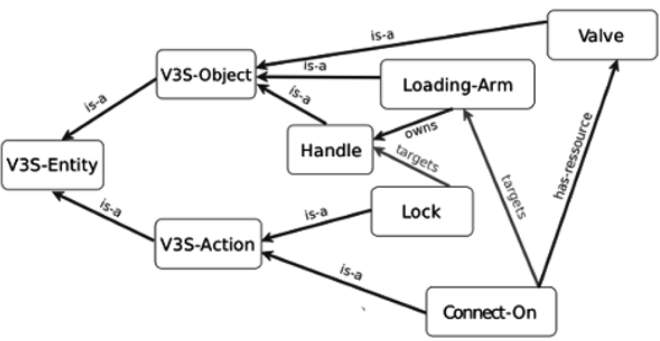
\includegraphics[width=0.5\linewidth]{figure/ontologyv3.png} 
  \begin{center}
  \cite{v3sframework}
  \end{center}
  \label{domainmodel}
\end{figure}

\textit{Activity Model} é estruturado sobre uma linguagem de descrição conhecido por \textit{ACTIVITY-DL}. Um dos elementos dessa linguagem é baseado na álgebra de Allen's que tem como finalidade definir raciocínios temporais \cite{allenalgebric}. As relações definidas por essa álgebra é dada por:

\begin{enumerate}
	\item $X < Y$ onde $X$: ocorre antes de $Y$ 
	\item $X m Y$,$Y mi X$: $X$ encontra $Y$
	\item $X o Y$, $X oi Y$: $X$ sobrepõem a $Y$
	\item $X s Y$, $Y si X$: $X$ começa $Y$
	\item $X d Y$, $Y di X$: $X$ ocorre durante $Y$	  
	\item $X f Y$, $Y fi X$: $X$ termina junto com $Y$	  	
	\item $X = Y$ $X$ é igual a $Y$	  		
\end{enumerate}

A \textit{Activity Model} define construtores que são semanticamente equivalente a certos operadores da álgebra de Allen's. Esses construtores (atuantes sobre atividades) são definidos pela Tabela \ref{acticonstruct}

\begin{table}[H]
\centering
\caption{Construtores da linguagem \textit{ACTIVITY-DL} \cite{v3sframework}}
\begin{tabular}{|l|l|l|}
\hline
Construtor & Nome         & Relações de Allen \\ \hline
IND        & Independent  & $A \{ <,>,m,mi,o,oi,s,si,d,di,f,fi,= \} B$\\ \hline
SEQ        & Sequential   & $A \{ <,>,m,mi \} B$\\ \hline
SEQ-ORD    & Ordered      & $A \{ <,>,m \} B$\\ \hline
PAR        & Parallel     & $A \{ o,oi,s,si,d,di,f,fi,= \} B$ \\ \hline
PAR-SIM    & Simultaneous & $A \{ = \} B$\\ \hline
PAR-START  & Start        & $A \{ s,si,= \} B$\\ \hline
PAR-END    & End          & $A \{ f,fi,= \} B$ \\ \hline
\end{tabular}
\label{acticonstruct}
\\
\begin{center}
Autoria Própria
\end{center}
\end{table}

As relações temporais entre as subatividades são especificadas por intermédio de construtores que são formalmente definidos no estudo \cite{allenalgebric}. Essas relações são intermediadas pelo vocábulo \textit{Pré-condição} que tem como propósito apresentar o contexto sobre qual uma atividade deve ser executada. A Tabela \ref{precondition} apresenta esses contextos.

\begin{table}[H]
\centering
\caption{As pré-condições possíveis para as atividades}
\begin{tabular}{|l|l|p{0.3\linewidth}|}
\hline
\textbf{Categoria} & \textbf{Pré-condição} & \textbf{Descrição}                                                                                                                                                                                                                                              \\ \hline
Condições para perceber  & Nomológico            & Descreve o estado de mundo necessário para que a tarefa seja fisicamente realizável. Condições dependem diretamente das regras de ação definidas no modelo de domínio. Exemplo: abre a porta se estiver fechada.                                                \\ \hline
Condições para perceber  & Regulamentar          & Descreve o estudo de mundo necessário para uma boa realização da atividade de acordo com prescrito em procedimento. Exemplo: para desconectar o tubo, as proteções devem ser desgastadas. \\ \hline
Condições para examinar & Contextual            & Descreve o estado de mundo em que a atividade é relevante. Quando essa condição é falsa, então a atividade deve ser ignorada. Exemplo: limpar o tubo é relevante apenas se o tubo estiver sujo.                                                                 \\ \hline
Condições para examinar & Favorável             & Descreve o estado de mundo onde a tarefa é preferencial sobre as demais. Essas condições ajudam a escolher entre várias tarefas quando existe uma alternativa para a realização de uma tarefa decomposta. Exemplo: se o parafuso estiver enferrujado, desarmar. \\ \hline
\end{tabular}
\begin{center}
\cite{v3sframework}
\end{center}
\label{precondition}
\end{table}

No que tange a questões referentes a segurança e violação, a linguagem \textit{ACTIVITY-DL} deve lidar com atividades em estados de alta degradação bem como com compromissos cognitivos  que são um grande potencial para a geração de risco. Essa condição possibilita a verificação de erros nos seguintes aspectos: atividades de aprendizagem e demonstração de comportamentos similares tendo como base personagens virtuais \cite{v3sframework}. Por conta disso, a linguagem \textit{ACTIVITY-DL} incorpora os conceitos de BCTUs e BATUs. Ambas tags trabalham com o fato de que, ao menos em partes, o profissional decide por cometer uma violação tendo em vista a inviabilidade (ou por não ser prático) efetuar a ação com base no que é definido pelos manuais. 

\textit{Risk Models} é a parte do modelo que define a análise de risco. Existem duas categorias: risco de análise clássico e método de análise de confiabilidade humana. A primeira categoria permite definir uma análise quantitativa de risco, contudo falha ao definir a complexidade dos resultados frente a fatores humanos. Em contrapartida, a segunda categoria considera fatores humanos, contudo falha em definir medidas objetivas sobre questões de segurança \cite{v3sframework}. O \textit{V3S} combina ambas situações usando a abordagem MELISSA \cite{melissaproject,v3sframework}. Essa abordagem é baseada em três pontos (1) atividades relacionadas em cenários de acidentes, (2) descrição das tarefas de representação e (3) fatores influentes em potencial nas atividades. MELISSA representa os cenário de acidente por meio do gráfico \textit{Bowtie}, o qual consiste na identificação de todos os cenários de acidentes bem como no provisionamento e uma listagem de barreiras para os mesmos. O risco aceitável consiste em escolhas que verificam o número e desempenho dessas barreiras. Os ponto central do gráfico de \textit{Bowtie} consiste em eventos críticos, a parte da esquerda desse gráfico implica as causas do evento e a parte direita do mesmo corresponde as consequências do evento \cite{v3sframework,melissaproject}. Essa descrição pode ser analisada na Figura \ref{bowtiegraf}. 


\begin{figure}[H]
  \centering
  \caption{Gráfico de Bowtie}
  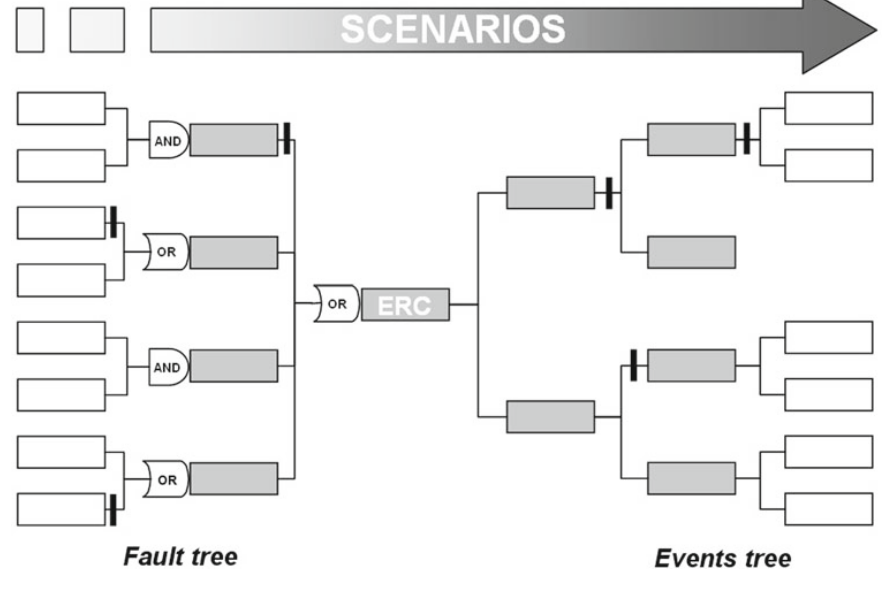
\includegraphics[width=0.5\linewidth]{figure/bowtie.png}
  \begin{center}
  \cite{melissaproject}
  \end{center} 
  \label{bowtiegraf}
\end{figure}


Com o propósito de gerar reflexões no que tange aos riscos de dada atividade, o \textit{V3S} trabalha com o conceito de personagens virtuais em um ambiente. Os raciocínios a cerca destes personagens são feitos usando um formalismo matemático denominado por redes de Petri, ou - mais especificamente Máquinas de Estado \cite{v3sframework} tendo como base simular a complexidade, flexibilidade e variabilidade de comportamentos que podem ser verificados em um ser humano. Por conta disso, os cientistas desse estudo decidiram modelar esse comportamento usando sistemas multi-agentes, mas especificamente um \textit{framework} conhecido como MASVERP (tratado na seção \ref{agent}).

O \textit{V3S} tem como finalidade providenciar um modelo que seja coerente, relevante, variado e eficiente em termos de cenário de treinamento com a finalidade de proporcionar atividades de aprendizagem. Esse modelo também apresenta um módulo que monitora cenários adaptativos conhecidos por \textit{HERA}. Em vez de interromper o usuário de forma sistemática a fim de explicar os seus erros, o \textit{framework} possibilita que o agente cometa erros e observe suas respectivas consequências no mundo virtual. Portanto, a dinâmica do cenário adaptativo permite trazer situações de treinamento relevantes. 

\textit{HERA}, por intermédio de regras baseadas em modelos pedagógicos, fornece o respaldo ao instrutor. Esse retorno é feito por intermédio dos seguintes critérios pedagógicos: escala de modificação - ampliar determinadas partes de um objeto com a finalidade de melhorar a visualização; reificação - verificar como o aprendiz lida com determinados conceitos e abstrações em termos concretos, restrições nos limites das ações do aprendiz que consistem em envio de mensagem ao agente quando ele comete sérios erros e superposição de informações se o aprendiz cometer e argumentar sobre as consequências das ações. \textit{HERA} é integrado ao módulo de reconhecimento que tem como finalidade usar técnicas que permitem redefinir as relações de atividades usando a linguagem \textit{ACTIVITY-DL} parametrizando-se nas ações, erros e violações. Essa parte do \textit{V3S} é capaz de distinguir entre os tipos de erros, que são: 1 - erros relacionados a atividades, 2 - erros relacionados ao ato de cumprir com o objetivo, 3 - erros de \textit{BATU}, 4 - erros de função e 5 - erros de ponto de vista.

	
		\textit{Activity Model} é estruturado sobre uma linguagem de descrição conhecido por \textit{ACTIVITY-DL}. Um dos elementos dessa linguagem é baseado na álgebra de Allen's que tem como por finalidade definir raciocínios temporais \cite{allenalgebric}. 
As relações definidas por essa álgebra é dada por; 

\begin{enumerate}
	\item $X < Y$ onde $X$: ocorre antes de $Y$ 
	\item $X m Y$,$Y mi X$: $X$ encontra $Y$
	\item $X o Y$, $X oi Y$: $X$ sobrepõem a $Y$
	\item $X s Y$, $Y si X$: $X$ começa $Y$
	\item $X d Y$, $Y di X$: $X$ ocorre durante $Y$	  
	\item $X f Y$, $Y fi X$: $X$ termina junto com $Y$	  	
	\item $X = Y$ $X$ é igual a $Y$	  		
\end{enumerate}

A \textit{Activity Model} define construtores que são semanticamente equivalente a certos operadores da álgebra de Allen's. Esses construtores (atuantes sobre atividades) são definidos pela tabela \ref{acticonstruct}

\begin{table}[H]
\centering
\begin{tabular}{|l|l|l|}
\hline
Construtor & Nome         & Relações de Allen \\ \hline
IND        & Independent  & $A \{ <,>,m,mi,o,oi,s,si,d,di,f,fi,= \} B$\\ \hline
SEQ        & Sequential   & $A \{ <,>,m,mi \} B$\\ \hline
SEQ-ORD    & Ordered      & $A \{ <,>,m \} B$\\ \hline
PAR        & Parallel     & $A \{ o,oi,s,si,d,di,f,fi,= \} B$ \\ \hline
PAR-SIM    & Simultaneous & $A \{ = \} B$\\ \hline
PAR-START  & Start        & $A \{ s,si,= \} B$\\ \hline
PAR-END    & End          & $A \{ f,fi,= \} B$ \\ \hline
\end{tabular}
\caption{Construtores da linguagem \textit{ACTIVITY-DL} \cite{v3sframework}}
\label{acticonstruct}
\end{table}

As relações temporais entre as sub-atividades são especificadas por intermédio de construtores que são formalmente definidos no estudo \cite{allenalgebric}. Essas relações são intermediadas pelo vocábulo \textit{Pré-condição} que tem como por propósito apresentar o contexto sobre qual uma dada atividade deve ser executada. A tabela \ref{precondition} apresenta esses contextos.

\begin{table}[H]
\begin{tabular}{|l|l|p{0.6\linewidth}|}
\hline
\textbf{Categoria} & \textbf{Pré-condição} & \textbf{Descrição}                                                                                                                                                                                                                                              \\ \hline
Condições para perceber  & Nomológico            & Descreve o estado do mundo necessário para que a tarefa seja fisicamente realizável. Condições dependem diretamente das regras de ação definidas no modelo de domínio. Exemplo: Abre a porta se estiver fechada.                                                \\ \hline
Condições para perceber  & Regulamentar          & Descreve o estudo do mundo necessário para uma boa realização da atividade de acordo com prescrito em procedimento. Exemplo: Para desconectar o tubo, a proteções devem ser desgastado.                                                                         \\ \hline
Condições para  Examinar & Contextual            & Descreve o estado de mundo em que a atividade é relevante. Quando essa condição é falsa, então a atividade deve ser ignorada. Exemplo: Limpar o tubo é relevante apenas se o tubo estiver sujo.                                                                 \\ \hline
Condições para  Examinar & Favorável             & Descreve o estado de mundo onde a tarefa é preferencial sobre as demais. Essas condições ajudam a escolher entre várias tarefas quando existe uma alternativa para a realização de uma tarefa decomposta. Exemplo: se o parafuso estiver enferrujado, desarmar. \\ \hline
\end{tabular}
\caption{As pré-condições possíveis para as atividades \cite{v3sframework}}
\label{precondition}
\end{table}


No que tange a questões referentes a segurança e violação, a linguagem \textit{ACTIVITY-DL} deve lidar com atividades em estados de alta degradação bem como com compromissos cognitivos  que são um grande potencial para a geração de risco. Essa condição possibilita a verificação de erros nos seguintes aspectos: atividades de aprendizagem e demonstração de comportamentos similares tendo como base personagens virtuais \cite{v3sframework}. Por conta disso, a linguagem \textit{ACTIVITY-DL} incorpora os conceitos de BCTUs e BATUs cujos fundamentos científicos estão descritos em \ref{risksec}. Ambas tags trabalham com o fato de que, ao menos em partes, o profissional decide por cometer uma dada violação tendo em vista a inviabilidade (ou por não ser prático) efetuar a ação com base no que é definido pelos manuais. 

\textit{Risk Models} é a parte do modelo que define a análise de risco. Existe duas categorias; risco de análise clássico e método de análise de confiabilidade humana. A primeira categoria permite definir uma análise quantitativa de risco, contudo falha ao definir a complexidade dos resultados frente a fatores humanos. Em contrapartida, a segunda categoria considera fatores humanos, contudo falha em definir medidas objetivas sobre questões de segurança \cite{v3sframework}. O \textit{V3S} combina ambas situações usando a abordagem MELISSA \cite{melissaproject} \cite{v3sframework}. Essa abordagem é baseada em três pontos (1) atividades relacionadas em cenários de acidentes, (2) descrição das tarefas de representação e (3) fatores influentes em potencial nas atividades. MELISSA representa os cenário de acidente por meio do gráfico \textit{Bowtie}. Isso consiste na identificação de todos os cenários de acidentes bem como no provisionamento e uma listagem de barreiras para os mesmos. O risco aceitável consiste em escolhas que verificam o número e desempenho dessas barreiras. Os ponto central do gráfico de \textit{Bowtie} consiste em eventos críticos, a parte a esquerda desse gráfico implica as causas do evento e a parte direita do mesmo corresponde as consequências do evento \cite{v3sframework}, \cite{melissaproject}. Essa descrição pode ser analisada na figura \ref{bowtiegraf}. 


\begin{figure}[H]
  \centering
  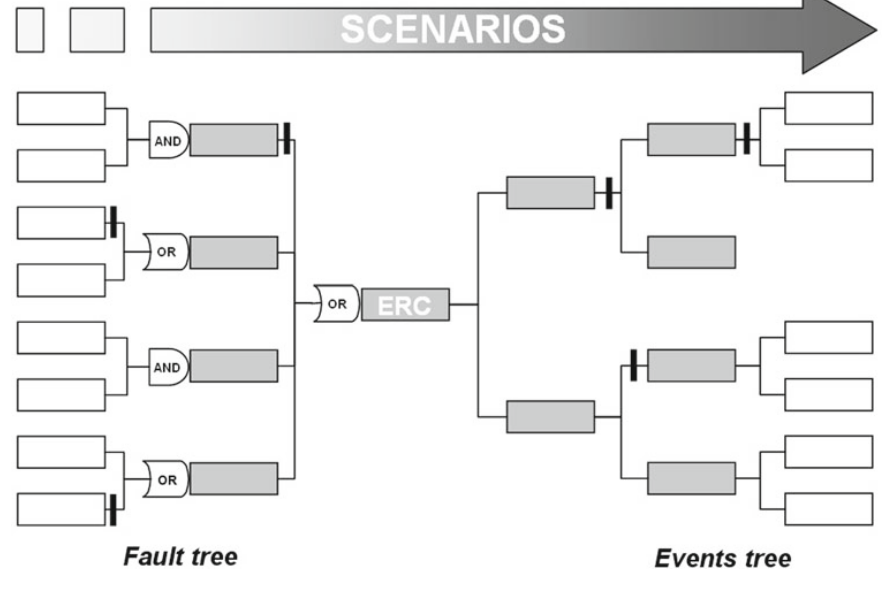
\includegraphics[width=0.5\linewidth]{figure/bowtie.png} 
  \caption{Gráfico de BowTie do texto \cite{melissaproject}}
  \label{bowtiegraf}
\end{figure}


Com o propósito de gerar reflexões no que tange aos riscos de dada atividade, o \textit{V3S} trabalha com o conceito de personagens virtuais em um ambiente. Os raciocínios a cerca destes personagens são feitos usando um formalismo matemático denominado por redes de Petri, ou - mais especificamente máquinas de estado \cite{v3sframework} tendo como base simular a complexidade, flexibilidade e variabilidade de comportamentos que podem ser verificados em um ser humano. Por conta disso, os cientistas desse estudo decidiram modelar esse comportamento usando sistemas multi-agentes, mas especificamente um \textit{framework} conhecido como MASVERP (tratado na seção \ref{agent}).

O \textit{V3S} tem como por finalidade providenciar um modelo que seja coerente, relevante, variado e eficiente em termos de cenário de treinamento com a finalidade de proporcionar atividades de aprendizagem. Esse modelo também apresenta um módulo que monitora cenários adaptativos conhecidos por \textit{HERA}.Em vez de interromper o usuário de forma sistemática a fim de explicar os erros dele, o framework possibilita que o agente cometa erros e observe suas respectivas consequências no mundo virtual. Portanto, a dinâmica do cenário adaptativo permite trazer situações de treinamento relevantes. 

\textit{HERA}, por intermédio de regras baseadas em modelos pedagógicos, fornece o respaldo ao instrutor. Esse retorno é feito por intermédio dos seguintes critérios pedagógicos; escala de modificação - amplia determinadas partes de um objeto com a finalidade de melhorar a visualização, reificação - verificar como o aprendiz lida com determinados conceitos e abstrações em termos concretos, restrições nos limites das ações do aprendiz que consiste em envio de mensagem ao agente quando ele comete sérios erros e superposição de informações se o aprendiz cometer e argumentar sobre as consequências das ações. \textit{HERA} é integrado ao módulo de reconhecimento que tem como por finalidade usar técnicas que permitem redefinir as relações de atividades usando a linguagem \textit{ACTIVITY-DL} se parametrizando nas açõe,s erros e violações. Essa parte do \textit{V3S} é capaz de distinguir entre os tipos de erros, que são: 1 - erros relacionados a atividades, 2 - erros relacionados ao ato de cumprir com o objetivo, 3 - erros de \textit{BATU}, 4 - erros de função e 5 - erros de ponto de vista.

As tables a seguir exibiem uma comparação entre o \textit{VS3} e o modelo proposto neste estudo.

\begin{table}[H]
\centering
\begin{tabular}{|l|p{0.3\linewidth}|p{0.3\linewidth}|}
\hline			
\textbf{Atributos}
& 
\textbf{VS3}
& 
\textbf{Modelo deste Estudo} 
\\ \hline
Finalidade
&
Representar cenários de Acidentes a fim de simula-los com propósito de treinamento profissional 
&
Representar cenários de Acidentes 
\\ \hline
Artefatos-Objetos
&
Representa objetos através da classe (da ontologia atrelada ao módulo \textit{Domain Model}) \textit{V3S-Object}
&
Representa objetos através do conjunto \textit{Artefact}
\\ \hline
Relações entre Entidades
&
Representa as relações entre objetos através da classe (da ontologia atrelada ao módulo \textit{Domain Model}) \textit{V3S-Action} através de relacionamentos com a classe \textit{V3S-Object}
&
Representa as relações entre as entidades através do predicado $possEntityRel(r_l,e_i,e_k)$
\\ \hline
Representação dos Objetivos
& 
Faz uso do modelo \textit{ACTIVITY-DL} - Permite expressar os seguintes racicínios; tarefas independentes, tarefas sequenciais, tarefas que se iniciam mediante a uma solicitação (pedido ou ordem), tarefas paralelas, tarefas  simultâneas, tarefas que se iniciam no mesmo instante e tarefas que são encerradas no mesmo instante)
&
Possui uma estrutura simples para representar objetivos que avalia apenas questões de pré-requisitos.
\\ \hline
\end{tabular}
\end{table}


\begin{table}[H]
\centering
\begin{tabular}{|l|p{0.3\linewidth}|p{0.3\linewidth}|}
\hline			
\textbf{Atributos}
& 
\textbf{VS3}
& 
\textbf{Modelo deste Estudo} 
\\ \hline
Riscos e Acidentes
&
Modelo \textit{MELISSA} (BATU E BCTU)
&
Uso de Normas, Violações, Sanções e Lógica Possibilistica aplicadas a contextos específicos por meio das regras \ref{conditionViol}, \ref{relationViol}, \ref{entityViol}, \ref{consconditionViol} e \ref{consrelationViol}
\\ \hline 
Agentes     	
& 
Uso do framework MASVERP 
& 
Não representar os processos mentais do agente 
\\ \hline 
Estrutura da Linguagem
& 
Diferentes formalismos da computação tais como; Ontologias, Lógica de Primeira Ordem, Algoritmos e entre outros
&
Teoria de Conjuntos e Lógica de Predicados
\\ \hline 
Estruturas para Avaliação e Treinamento
& 
HERA
&
Não Consta
\\ \hline
\end{tabular}
\end{table}
	
		\section{Modelo NormMAS}
\textit{NormMAS} é um modelo usado para definir comportamento normativo de sistemas multiagentes \cite{normas}. No que tange questões referentes ao comportamento normativo, o modelo trabalha com duas definições \cite{normas}.

		
		\textbf{Definição 1.} \textit{Um norma é definida por meio de uma tupla} $N = \langle \mu,\kappa,\chi,\tau,\rho \rangle$

\begin{itemize}
    \item $\mu \in \{obligation,prohibition\}$ representa as modalidades de norma.
    \item $\kappa \in \{action,state\}$ representa o tipo de \textit{trigger} da condição.
    \item $\chi$ representa o conjunto de estados em que uma norma se aplica.
    \item $\tau$ representa a norma da condição de \textit{trigger}
    \item $\rho$ representa a sanção aplicava pela violação do agente.
\end{itemize}

A definição 1 pode ser compreendida sobre o seguinte exemplo; 

\textit{Todos os imigrantes que possuem passaporte válido, devem ser aceitos. A falha resulta na perda de 5 créditos}. 

Dentro da definição 1, o exemplo fica;

\begin{eqnarray} 
    \langle obligation,action,valid(Passport),accept(Passport),loss(5)\rangle
\end{eqnarray}

\textit{NormMAS} define um \textit{Registro de ação} que é dado pela definição 2. 

\textbf{Definição 2.} \textit{Um Registro de Ação é definido por meio de uma tupla} $R = \langle \gamma,\alpha,\beta \rangle$

\begin{itemize}
    \item $\gamma$ representa o agente executando uma ação;
    \item $\alpha$ representa a ação sendo executada pelo agente $\gamma$
    \item $\beta$ representa os estados internos do agente $\gamma$ no momento da execução.
\end{itemize}

Para demonstrar como se dá o uso dessa definição pode-se considerar a seguinte sentença;

\textit{O oficial John aprovou passaport 3225. O passaporte 3225 é definido como validado.}

Nessa sentença, $John$ é o agente dado por $\gamma$, o ato de aprovar o passaporte é o $\gamma$ que pode ser definido pelo predicado por $approve(3225)$ e o estado de ser validado por ser dado pelo predicado $valid(3225)$.  

Usando a \textbf{Definição 2}, isso poder ser especificado da seguinte maneira; 

\begin{eqnarray} 
    \langle John, approve(3225), valid(3225)\rangle
\end{eqnarray}

As tabelas a seguir exibem uma comparação entre o \textit{NORMMAS} e o modelo proposto neste estudo.

\begin{table}[H]
\centering
\begin{tabular}{|l|p{0.3\linewidth}|p{0.3\linewidth}|}
\hline          
\textbf{Atributos}
& 
\textbf{NORMMAS}
& 
\textbf{Modelo deste Estudo} 
\\ \hline
Finalidade
&
Representar agentes considerando questões atreladas a Normas, Sanções e Violações
&
Representar cenários de Acidentes 
\\ \hline
Generalização
&
Trata de cenários onde se tem o interesse de representar agentes, normas, violações e sanções. 
&
Trata de cenários específicos para acidentes onde se deseja as causas do acidente. 
\\ \hline
Agentes
&
Não define os estados mentais do agente
&
Não define os estados mentais do agente
\\ \hline
Representação de Objetivos
& 
Não possui estrutura para representar objetivos
&
Possui uma estrutura simples para representar objetivos. Essa estrutura considera apenas questões de pré-requisitos. 
\\ \hline
Normas 
&
Presença de tuplas que permite expressar proibições e sanções para os mais diversos casos possíveis. 
&
Presença de regras que permite expressar violações e sanções para cenários de acidentes.
\\ \hline
Generalização
&
Trata de cenários onde se tem o interesse de representar agentes, normas, violações e sanções. 
&
Trata de cenários específicos para acidentes onde se desejeva verificar as causas do acidente.
\\ \hline
Estrutura da Linguagem
& 
Lógica de Primeira Ordem (definições dos conceitos em termos de Tuplas)
&
Teoria de Conjuntos e Lógica de Predicados  
\\ \hline
\end{tabular}
\end{table}
		
		\subsection{NORMMAS}

A tabela a seguir exibem uma comparação entre o \textit{NORMMAS} e o modelo proposto neste estudo.

\begin{table}[H]
\centering
\begin{tabular}{|l|p{0.3\linewidth}|p{0.3\linewidth}|}
\hline          
\textbf{Atributos}
& 
\textbf{NORMMAS}
& 
\textbf{Modelo deste Estudo} 
\\ \hline
Finalidade
&
Representar agentes considerando questões atreladas a Normas, Sanções e Violações
&
Representar cenários de Acidentes 
\\ \hline
Generalização
&
Trata de cenários onde se tem o interesse de representar agentes, normas, violações e sanções. 
&
Trata de cenários específicos para acidentes onde se deseja as causas do acidente. 
\\ \hline
Agentes
&
Não define os estados mentais do agente
&
Não define os estados mentais do agente
\\ \hline
Representação de Objetivos
& 
Não possui estrutura para representar objetivos
&
Possui uma estrutura simples para representar objetivos. Essa estrutura considera apenas questões de pré-requisitos. 
\\ \hline
Normas 
&
Presença de tuplas que permite expressar proibições e sanções para os mais diversos casos possíveis. 
&
Presença de regras que permite expressar violações e sanções para cenários de acidentes.
\\ \hline
Generalização
&
Trata de cenários onde se tem o interesse de representar agentes, normas, violações e sanções. 
&
Trata de cenários específicos para acidentes onde se desejeva verificar as causas do acidente.
\\ \hline
Estrutura da Linguagem
& 
Lógica de Primeira Ordem (definições dos conceitos em termos de Tuplas)
&
Teoria de Conjuntos e Lógica de Predicados  
\\ \hline
\end{tabular}
\end{table}

\subsection{Comparação Genérica entre os Modelos}

Tendo como base as análises feitas nas seções anteriores, é possível chegar na tabela \ref{comparemodel} que apresenta uma análise comparativa dos arcabouços no que tange a expressividade do modelo computacional proposto nesse texto. Por expressividade, se entende capacidade de expressar, representar o objeto de interesse. Para essa análise 
foi feita a seguinte escala: nenhuma expressividade $\prec$ pouco expressivo $\prec$ expressivo $\prec$ muito expressivo $\prec$ altamente expressivo. O termo nenhuma expressividade não indica que é impossível definir a estrutura em observação dentro do modelo em voga, mas sim que o engenheiro de modelagem terá que criar uma estrutura conceitual ad hoc. Sobre o mesmo aspecto reside pouco expressivo, contudo o modelo - neste caso - possui algumas estruturas pré-definidas que diminuem o esforço da especificação. O termo expressivo deixa claro que o modelo permite especificar o objeto de interesse sem que o engenheiro tenha de criar muitos atributos para o domínio de interesse. O termo muito expressivo define que o modelo apresenta diversos conceitos específicos para representar o objeto em interesse, contudo ainda há margem para que o modelador tenha que criar um ou mais atributos. O termo altamente expressivo define o caso onde o modelo especifica o objetivo de interesse muito bem fazendo com que o modelador não precise definir nenhum critério conceitual a mais (ou terá que montar poucas definições).   

\begin{table}[H]
    \centering
    \scalefont{0.6}
    \begin{tabular}{|l|l|l|l|l|}
        \hline
        \textbf{Critérios} & \textbf{MOISE+}        & \textbf{DASTANI}     & \textbf{V3S}         & \textbf{NORMMAS}          \\ \hline
        \textbf{Agente}    & pouco                  & pouco                & muito                & pouco                     \\ \hline
        \textbf{SMA}       & altamente              & pouco                & expressivo           & pouco                     \\ \hline
        \textbf{Artefato}  & nenhuma                & pouco                & expressivo           & pouco                     \\ \hline
        \textbf{Norma}     & nenhuma                & altamente            & pouco                & altamente                 \\ \hline
        \textbf{Violação}  & nenhuma                & altamente            & pouco                & altamente                 \\ \hline
        \textbf{Sanção}    & nenhuma                & altamente            & pouco                & altamente                 \\ \hline
        \textbf{Risco}     & nenhuma                & pouco                & altamente            & pouco                     \\ \hline
        \textbf{P.O.A.E}   & nenhuma                & pouco                & pouco                & pouco                     \\ \hline
        \textbf{Objetivos} & muito                  & pouco                & muito                & pouco                     \\ \hline
        \textbf{C.A}       & nenhuma                & pouco                & pouco                & pouco                     \\ \hline
        \textbf{I.AG.AR}   & nenhuma                & pouco                & pouco                & pouco                    \\ \hline
        \textbf{D.C.A}     & nenhuma                & pouco                & altamente            & pouco 
    \\ \hline
    \end{tabular}
    \caption{Análise comparativa sobre a expressividade desses modelos no que tange aos objetivos deste estudo. A sigla P.E.R significa Possibilidade de Algo Errado, a sigla C.A consiste em 
    Condições Ambientes, a sigla I.AG.AR significa Interação entre Agente e Artefato e a sigla D.C.A significa Descrição de Cenário de Acidente}
    \label{comparemodel}
\end{table}

O critério \textbf{Agente} condiz com representação dos estados internos que um agente pode ter. O critério \textbf{SMA} condiz com presença de elementos que são necessários para especificar um \textit{Sistema Multiagente}. O critério \textbf{Artefato} condiz com elementos que correspondem a definição presente na seção \ref{artefact}. O critérios de \textbf{Norma} corresponde a regras que devem ser acatadas pelos agentes. \textbf{Violação} define o que corresponde o não cumprimento de uma dada regra. \textbf{Sanção} implica penalidade que está sobre o agente. \textbf{Risco} consiste no evento ruim que tem um potencial de ocorrer sobre o agente. \textbf{P.O.A.E} significa Possibilidade de Ocorrer algo Errado e corresponde a expressar condições onde existe potencial de acontecer algo inapropriado sobre o agente mesmo que esse realize sua função com excelência.  \textbf{Objetivos} implica alvos que devem ser atingidos pelos agentes. \textbf{C.A} consiste em condições ambientes que interagem com a atividade executada pelos agentes. \textbf{I.AG.AR} representa as interações entre agentes e artefatos. \textbf{D.C.A} - Descrição de Cenários de Acidentes, consiste na capacidade de desenvolver raciocínios a fim de representar cenários de acidentes.

As subseções anteriores em conjunto com a tabela \ref{comparemodel} permitem concluir que esse trabalho é inovador no que tange a ter um vocabulário específico para representar cenários de risco e de acidentes (tanto sobre o responsável pelo acidente bem como a vitima) de atividades manuais usando para isso, o conceito de sistema multiagente normativo. Esse vocabulário apresenta limitações as quais serão debatidas na próxima seção. 
		

	\section{Consistência dos Resultados}\label{constresult}

		A discussão dos resultados que estão expostos nas sub-seções \ref{mods}, \ref{predic}, \ref{regras} foi feita na própria apresentação dos mesmos. Isso se deve a natureza desses resultados , não é possível realizar a exposição deles sem discutir os fundamentos conceituais que justifiquem a existência dos mesmos. Essa situação não se aplica no texto presente em \ref{studycase} e em \ref{rac} onde os resultados estão apenas expostos mas não foram discutidos. O mesmo acontece com a Metodologia usada para chegar nesses resultados, foi exposta mas não foi discutida. O texto a seguir fará uma discussão desses elementos apresentando as principais dificuldades que foram encontradas na realização desse estudo. 

\subsection{Considerações sobre Critérios Metodológicos ao estudo de caso} \label{conscritmetcasoestudo}

A primeira fase consistiu em descrever a manutenção em termos de objetivos que as vezes são organizados em série e as vezes em paralelo. Não houve grandes dificuldades para fazer isso, pois essa atividade é claramente composta de subatividades. O que foi um ponto relativamente complicado de se verificar nesse estudo, é que os profissionais não precisam executar os objetivos na estrutura em que o modelo foi apresentado. Inclusive, muitas vezes os técnicos planejam a manutenção de um jeito e ao chegar no ambiente de execução eles mudam o encadeamento dos objetivos. Há um número finito e relativamente pequeno (é difícil definir um número, mas as observações permitem concluir que este número está na ordem de 10 formas diferentes) sobre como esses objetivos podem ser organizados e isso ameniza a falta de previsibilidade de como a manutenção será realizada. 

O problema da organização dos objetivos pode ser resolvida de três maneiras diferentes. Em uma delas o engenheiro de manutenção modela o problema para todos os cenários possíveis. Portanto, se houver 10 formas diferentes de organizar esses objetivos, o engenheiro deverá refletir acerca dessas 10 formas. Outra forma consiste em definir todas as relações possíveis que o predicado $nextGoal(g_i,g_j)$ permite em uma única estrutura. Nessa implementação do modelo, o agente por intermédio dos seus estados internos, escolhe a qual objetivo ele deverá tentar alcançar. Essa questão não foi levada em consideração no estudo de caso em análise porque o autor estava interessados em realizar a análise necessária sobre a possibilidade de usar este modelo em um problema real. É possível argumentar que aquele arranjo de objetivos não é o único possível, contudo não deixa de ser um arranjo real e que pode servir de referência aos profissionais. A terceira solução a ser considerara consiste no estudo e uso de algoritmos de \textit{Partial Order Planning} aplicados a essa problemática \cite{planning}. 

O autor desse estudo não sabe afirmar se o arranjo dos objetivos interferem no predicado $affectsRels(r_k,r_n)$. Para que isso seja analisado se faz necessário aplicar esse modelo para diversas situações diferentes onde todas devem apresentar a problemática do arranjo de objetivos. Se em uma dessas situações a especificação do predicado $affectsRels(r_k,r_n)$ mudar, então a proposição - o arranjo de objetivos que afeta o predicado $affectsRels(r_k,r_n)$) - deve ser tida como verdadeira, contudo se não mudar, não é possível afirmar que essa proposição é falsa. 

A utilização do conceito de papel e da relação entre o agente e o seu papel foram muito adequados para as análises desse modelo. Isso se deu por observar como ocorre a distribuição dos objetivos aos agentes. Isso, pois na manutenção em linha viva todos os profissionais são tidos como executores, contudo existe uma distribuição de tarefas tendo em vista o conhecimento e a experiência de cada profissional ali envolvido. Portanto, para enquadrar essa questão nos moldes do modelo em análise se fez necessário encontrar um padrão de como os objetivos são distribuídos em função das atividades dos agentes. Com base nisso o autor concluiu o que está exposto na Tabela \ref{agentsroles}.

Os conceitos de artefato e de relação foram adequados para esse estudo de caso não tendo a necessidade de definir nenhuma outra abordagem para isso. Todo o rol de ferramentas e de equipamentos foram definidos como artefatos. A fim de tornar a modelagem mais expressiva, o autor desta dissertação criou subconjuntos de artefatos definindo um apenas para ferramentas e outro apenas para equipamentos. Isso não foi feito para não induzir os leitores desse estudo ao erro por entender que essa divisão pertence a estrutura conceitual do modelo propriamente dito. Uma taxonomia dessas seria adequada apenas para esse caso em estudo, caso contrário diminuiria o poder de generalização do modelo. 

Os conceitos de condição, risco e consequência bem como predicado $hasRisk(c_k,risk_k,cs_m)$ cujas instâncias e o relacionamento do predicado para o estudo de caso são apresentados na Tabela \ref{condition} foram muito apropriados tanto no contexto do modelo em si como também em aplicação ao caso de estudo. Isso se deve ao fato de que uma condição não é um agente e não é um artefato mas é algo que está presente no meio da atividade e interfere com grande intensidade no andamento dos processos, portanto desconsiderar esse conceito ou compactá-lo como parte de outras estruturas implicaria uma representação míope da realidade. O autor entende que essas condições são o suficiente para poder realizar a representação desse modelo. As relações entre condição, risco e consequência foram apropriadas para representar diversos cenários dentro do estudo de caso. 

Uma consideraçao que deve ser feita sobre os conceitos de risco e consequência (cujas instâncias para o estudo de caso estão apresentadas nas Tabelas \ref{condition}, \ref{relationEntEnt1}) em relação ao estudo de caso é a de que foi considerado apenas um único risco, que é o de ser eletrocutado e uma única consequência, que é a morte. Contudo, há considerações que devem ser feitas no que tange a realidade, pois essa atividade exibe outros riscos tais como: queda, animais peçonhentos, queimadura entre outros que, assim como eletrocutado, podem apresentar outras consequências além da morte. Esses riscos a mais não foram considerados no caso em estudo porque os raciocínios exibidos na subseção \ref{rac} puderam ser feitos sem a necessidade deles. Outro ponto que corroborou com isso consiste no fato de que o autor estava interessados em obter primeiramente uma versão mais simples do modelo para então, se necessário, torná-lo mais complexo. Isso implica em realizar algumas escolhas pragmáticas e uma delas consiste na verificação de qual risco é o mais importante e o mais temeroso na atividade. A análise com os profissionais mostram que o risco de ser eletrocutado é o principal e é mais preocupante ao executar uma atividade de manutenção em linha viva. Outro ponto reside na verificação das consequências desse risco o que remete a uma pergunta: Um profissional de linha viva ao executar manutenção em uma subestação de energia pode se envolver em um acidente em que ele é eletrocutado, e ainda sobreviver? A resposta a essa pergunta é sim, porém muito improvável. Descargas de equipamentos que operam a 69 kV 1500 kVA  (o que é relativamente baixo) costumam matar o profissional eletrocutado mesmo que os disjuntores atuem na ordem de milissegundos. Portanto, outras consequências além da morte tal como: queimaduras e perda de membros, contudo na grande maioria dos casos o profissional recairá no óbito. 

O predicado $possEntityRel(r_l,e_i,e_k)$, em que as instâncias para o estudo de caso são apresentada na tabela \ref{relationEntEnt1}, define como se dá a relação entre duas entidades. Essa estrutura se tornou muito útil para fazer diversos raciocínios interessantes que estão presentes nas regras. Portanto o autor desta dissertação conclui que ela foi adequada, necessária e importante para essa representação e para esse estudo de caso, contudo, ela tornou a especificação da modelagem um processo muito custoso, porque o modelador teve de refletir em todas as relações possíveis que são executadas na atividade e depois disso, teve que ver quais relações se enquadravam em cada objetivo. Esse custo também está presente nos raciocínios que devem ser feitos pois dependendo da situação há uma série de relações que devem ser avaliadas. Essa questão nos permite refletir sobre a viabilidade de um modelo assim, para situações onde o número de artefatos bem como o número de relações entre esses artefatos tendem ao infinito. Contudo, o fato do modelador ter que refletir sobre todas as relações bem como seus respectivos riscos, permite a realização de uma análise muito mais profunda da atividade e de como a segurança dos profissionais pode ser afetada de situação para situação. 

O predicado $affectsRels(r_k,r_n)$ (cujas instâncias dos conceitos bem como a relação está presente na Tabela \ref{relation1}) agregou dificuldades tanto na concepção como na aplicação ao estudo de caso. Houve muitas tentativas de resolver essa questão sem ter que abstrair tanto quanto esse predicado faz. Contudo, realizar um mapeamento minucioso de como se dão as atividades, resulta em uma carga de trabalho relativamente custosa e que pode apresentar diversas fragilidades no que tange à consistência lógica (ou seja, um sistema que se contradiz). Portanto, em uma primeira abordagem, admitir que a não execução (ou a má execução) de uma relação afeta negativamente outra relação implica uma visão pragmática e simples para resolver o problema onde um eletricista se envolve em um acidente sobre o qual ele não tem responsabilidade alguma. O autor desse estudo admite que esse é um ponto do modelo a ser melhorado a fim de se obter representações consistentes, expressivas e em com relativo baixo custo de modelagem. 

Os predicados $requiresCirc(circ_n,g_m)$, $requiresEntity(goal_i, e_j)$, $instanceOfRel(circ_n)$ e $instanceOfCond(circ_n)$ (em que as instâncias para esses predicados estão presentes em \ref{relationsgroup1} e \ref{entitygoals}) apresentam a especificação dos relacionamentos entre entidades, relações e condições com os objetivos. O lado positivo dessa abordagem é a possibilidade de ter uma descrição lógico-formal da manutenção altamente detalhada. Isso permite a equipe responsável pela manutenção avaliar o problema com mais profundidade e, portanto, tomar decisões mais eficientes. O problema dessa abordagem reside na mesma situação atrelada à Tabela \ref{relationEntEnt1} que consiste em um processo altamente custoso em termos de tempo e de trabalho a fim de especificar as relações, entidades e condições com os objetivos. 

\subsection{Considerações sobre Critérios Metodológicos ao Raciocínios} \label{conscritmetrac}

Os raciocínios feitos sobre o modelo são de crucial importância para definir a eficácia desse projeto pois é com base nisso que se torna possível avaliar o quão efetivo vem a ser essa representação. Os raciocínios 1 e 5, dados respectivamente pelas subsubseções \ref{raciocinio1} e \ref{raciocinio5} apresentam o problema com bastante expressividade. Tendo em vista o fato de que a Glicerina  é um composto químico relevante para manter o isolamento da parte não condutiva do bastão universal, esquecer de realizar isso gera um potencial acidente de ser eletrocutado em todas as outras situações onde o bastão será usado (a não ser nas situações onde o bastão universal não será usado em condutores energizados). Tanto os predicados como as regras que estão atreladas a violação de relação e suas respectivas consequências representaram essa condição com sucesso. Nesse caso não aconteceu nenhuma sanção sobre o agente 4, portanto nem toda violação de relação gera necessariamente uma sanção. O predicado $possOfNegConseqFor$ conseguiu trazer com êxito a sensação de possibilidade que existe em fenômeno desse gênero. 

Quando o autor concebeu esse modelo, considerou a possibilidade de trabalhar problemas dos raciocínios 1 e 5 por meio do conceito de \textit{Probabilidade}. Isso é interessante porque um predicado que consegue expressar fenômenos estatísticos válidos com excelência, apresenta possibilidades de aplicações extremamente elevadas. Contudo, trabalhar com probabilidade resulta em diversas complicações de modelagem. Uma dessas complicações consiste na coleta de dados de uma amostragem significativa de uma população de acidentes e na análise estatística adequada para descrever a probabilidade de um acidente acontecer. Entretanto, isso não é o suficiente pois essa probabilidade é condicionada a ocorrência de uma determinada relação. O raciocínio 1, por exemplo, demonstra que a não execução de $relPanoGlicerina$ resulta na possibilidade de ocorrer um acidente em $relBastaoGarraGondutor$. Se o autor estivesse trabalhando com o conceito de probabilidade, então é necessário desenvolver técnicas que verificam a probabilidade de acontecer algo ruim na relação $relBastaoGarraGondutor$ para o caso da relação $relPanoGlicerina$ não ser efetivada com sucesso. Contudo, se a não execução de uma outra relação também afetar $relBastaoGarraGondutor$, então também se faz necessário encontrar essa outra probabilidade. Além de aumentar a complexidade desse modelo, abre diversas indagações no que tange a como fazer isso, o que pode ser um potencial campo de investigação científica. Com a finalidade de viabilizar uma primeira versão do modelo, o autor optou por usar o conceito de possibilidade em vez de probabilidade. Apesar de diminuir a expressividade do modelo no que tange a questão que existe um componente sobre aleatoriedade, isso simplifica o processo de especificação, facilita o desenvolvimento de raciocínios e evita que o modelo seja estruturado sob proposições falsas (por exemplo, definir uma probabilidade para uma condição de mundo que não é precisamente valorada). 

O vocabulário definido neste modelo foi apropriado para representar a condição de mundo presente no Raciocínio 2 que está exposto na subsubseção \ref{raciocinio2}. Em uma situação onde não há um pano para poder limpar todas as ferramentas, a manutenção é interrompida e essa situação ficou claramente representada por esse raciocínio onde a geração da violação de entidades corresponde a finalização da manutenção. Há a possibilidade de existir um cenário onde os profissionais criam algum tipo de técnica alternativa para poder transpassar a falta de algum artefato, inclusive se esse não apresentar grande complexidade estrutural como é o caso de um pano. Contudo, o autor decidiu por não incorporar esse tipo de situação no modelo por conta de complexidades que isso pode trazer a estrutura da representação. Manter o modelo assim permite representar os cenários mais prováveis, tendo vista que a ausência de diversos tipos de artefatos muitas vezes não permite a continuidade da atividade.    

A execução de uma manutenção em linha viva deve seguir a risca as condições ambientais adequadas para essa finalidade. Uma dessas condições é a umidade relativa do ar, que deve estar necessariamente inferior a setenta por cento. O raciocínio 3 em \ref{raciocinio3} demonstra esse tipo de situação onde um agente tenta executar uma atividade com a umidade relativa dor ar em níveis inapropriados para isso, ocasionando o surgimento de uma violação de condição gerando uma sanção no agente que corresponde a ser eletrocutado e, consequentemente, morto. É interessante observar que nem toda violação de condição, no mundo real, resulta necessariamente em uma sanção ao violador. A umidade relativa do ar recai nessa situação, pois pode ser que o profissional cometa essa violação sem se envolver em um acidente. Isso pode ser resolvido por construir regras tratando condições em relação ao predicado $possOfNegConseqFor$. Contudo, a desobediência de condições ambientes normalmente resultam em acidentes. Portanto, essa condição - apesar de não tratar todos os cenários possíveis, trata um bom número dos mesmos.

A chave catraca é usada pelo profissional de linha viva para remover um parafuso que está preso ao conector. Uma execução inapropriada dessa relação resulta na ocorrência do eletricista ser eletrocutado e morto. Há diversas formas de como isso pode acontecer, sendo que uma delas consiste no profissional se posicionar de forma inapropriada para realizar essa relação e, por consequência, esbarrar tanto com o corpo quanto com a ferramenta em algum condutor de forma inapropriada. Portanto é de crucial importância que o profissional realize a execução com excelência. Esse comportamento é descrito pelo Raciocínio dado na subsubseção \ref{raciocinio4}. Assim como na situação relacionada condição, a realidade dos fatos pode produzir cenários possíveis "nesse caso" que não são adequadamente representados por esse modelo. Um possível cenário para essa situação consiste no fato do profissional simplesmente não conseguir executar a relação, sem que isso resulte em algum acidente. Contudo, a situação descrita pelo modelo apresenta o pior cenário possível. 

Em um acidente pessoas que não são responsáveis por atos cometidos podem sofrer duras consequências desses atos. Essa situação está demonstrada no raciocínio 5 presente na subsubseção \ref{raciocinio5}. Nessa situação, não passar glicerina no pano pode gerar um acidente ao montar a relação parafuso conector, porque o bastão isolante a ser usado nesse  processo, não estará em condições operacionais seguras, uma vez que a superfície dessa ferramenta pode conter algum tipo de impureza que corrobore com aumento de corrente de fuga em níveis suficientemente altos para matar alguém. O raciocínio 1 apresentou com excelência essa influência que a falta do uso de glicerina tem sobre a possibilidade de ocorrer algo errado no momento em que um certo profissional remover o parafuso usando o bastão. O autor entende, portanto que todos os predicados usados para representar essa situação foram necessários sendo que a ausência de um ou de outro, descaracteriza completamente essa representação. Nessa condição, se faz necessário saber com qual objetivo $relParafusoConector$ está atrelado, e isso é feito por intermédio do $\in$ e de $requiresCirc(goal_i,circ_j)$. Além disso, não é possível efetuar nenhum tipo de raciocínio sobre essa condição sem levar em consideração se os agentes tentam alcançar esse objetivo, e isso é feito por meio do predicado $starts(agent_n,g_m)$. O fato de ocorrer um acidente, ser independente do agente que está executando o objetivo, é muito bem representado pelos predicados $possOfNegConseqFor$ e $happensNegConseqFor$. Pela regra \ref{paybutiamnotguilty}, essa reunião de fatores em conjunto com os riscos associados ao evento dão como verdade para o predicado $possOfNegConseqForEven$ gerando a morte do profissional e a interrupção da manutenção. 

A presença do raciocínio 6 dado em \ref{raciocinio6} demonstrou que o modelo é capaz de interpretar quando o objetivo $g23$ for atingido. Em conjunto com o predicado $enabledToStart(ag_i,g_j)$, com a programação dos estados internos do agente e com a regra \ref{rolenextgoal} é possível verificar uma relação de continuidade para a representação (desde que o modelador defina os critérios que levam o agente a tentar atingir um dado objetivo). 

O raciocínio 7 dado por \ref{raciocinio7} apresenta como o modelo se comporta quando é feito uma consulta que não corresponde a realidade, ou seja quando $agente1$ tente alcançar o objetivo $g23$ sendo que este não faz parte dos objetivos que devem ser alcançados por aquele. O resultado objetivo foi o que o autor esperava. 

O autor conclui que o estudo de caso foi representado de forma apropriada pelos predicados e regras presentes nesse texto. Contudo, muitos raciocínios não foram capazes de apresentar todos os cenários possíveis a uma dada circunstância. Porém, todos os cenários resultantes do modelo correspondem a circunstâncias reais da manutenção. Não apenas isso, mas são tanto as circunstâncias mais prováveis como as mais sérias. Assim sendo, escapa ao poder de modelo representar muitos cenários, contudo os cenários mais importantes foram muito bem computados por essa representação.

	\section{Aplicações}\label{application}
		
		Essa representação pode ser usada para conceber uma especificação a fim de por usar um dado arcabouço com o propósito de  desenvolvimento de sistemas de informação com muitas possíveis finalidades diferentes. Uma dessas finalidades implica desenvolver um sistema para realizar o planejamento de atividades com o propósito de fazer uma análise dos riscos possíveis. Isso, pois ao especificar uma dada atividade profissional nos moldes desse modelo, o modelador é induzido ao raciocínio de estruturar a atividade em forma de objetivos, é induzido a pensar em todas as entidades e relações importantes, e deve refletir nos riscos e consequências de cada relação e condição. 

Uma outra aplicação para esse modelo consiste em simular as atividades de interesse. 
Essa situação permite que os engenheiros de modelagem realizem diferentes cenários a fim de entender o que realmente acontece com os profissionais nessas condições. Criar um sistema \textit{mobile} para celular (ou qualquer outra forma de computador móvel) a fim de auxiliar os profissionais na execução de uma dada atividade também é outra possível aplicação desse modelo. Por ultimo, esse modelo apresenta potencial para ser usado em jogos sérios com a finalidade de emular algum dado procedimento a fim 
de analisar como os profissionais se comportam em condições de risco. 

Esse estudo fez uso da linguagem de programação \textit{PROLOG} para analisar um estudo de caso. Contudo, outras linguagens podem ser usadas para essa finalidade. Uma dessas é \textit{SQL} onde as classes podem ser definidas por meio de tabelas, as relações entre as classes por meio de chaves estrangeiras e as instâncias por meio de registros. As regras podem ser resolvidas por meio de consultas específicas que são definidas em tabelas temporárias usando condicionadores sentenciais \textit{if ... them ...} em procedimentos específicos para isso. Contudo, a maneira mais prática de tratar as regras consiste em escrevê-las em alguma linguagem de programação (estruturado em um algoritmo) que realiza consulta ao banco com as tabelas e relacionamentos do modelo. 

Bancos não relacionais com \textit{MONGO-DB} (usa a estrutura de dados em grafo conhecido com \textit{JSON}) também são apropriados para esse tipo de situação. Esse tipo 
de banco não usa relacionamentos o que apresenta uma dificuldade a mais para a implementação de um modelo dessa natureza, contudo isso pode ser resolvido por forçar os relacionamentos artificialmente na estrutura do banco permitindo consultas similares as presentes em \textit{SQL}.

Linguagens de programação orientadas a objeto (Java, C$\#$, PHP, C++) também são apropriadas para esse tipo de situação. As classes do modelo podem ser representadas pelas classes da linguagem e os relacionamentos podem ser concebidos por intermédio de métodos. O código pode apresentar um módulo que contem todas as regras do modelo. Assim, 
para cada evento que acontece no sistema, todas as regras são consultadas computando a solução para o dado de entrada. Nessa situação, a especificação é feita instanciando as classes. 

A natureza da implementação deverá ser ponderada com base no uso final do sistema. Para uma situação onde os profissionais necessitam de um sistema para planejar a manutenção, fazer uso de uma estrutura onde a especificação e os relacionamentos são definidos em banco de dados e as regras são estruturada em uma linguagem de programação é o melhor caminho. Isso, pois os profissionais terão de escrever registros no sistema diversas vezes durante o seu respectivo uso e isso necessita de uma estrutura preparada para esse trânsito de informação. Em contrapartida, deixar as regras em prol da linguagem de programação permite que o sistema efetive os raciocínios de maneira muito mais rápida quando houver necessidade. Nesse modelo o sistema realiza a consulta necessária ao banco de dados, escreve o retorno na memória \textit{RAM} e o computa
nas regras. 

Se a implementação dessa representação for usada em um jogo de computador, escrever as classes, relacionamentos, instâncias e regras em uma linguagem de programação eliminando o uso de banco de dados é a alternativa mais interessante nessa situação. Isso se deve ao fato de que muitas vezes um jogo necessita de alto desempenho para funcionar. Eliminar o banco de dados evita o tempo de consulta a memórias lentas remove um custo computacional significativo. Se se os profissionais optarem por manter um banco de dados, devem tentar resolver a situação com o menor número de consultas possíveis - talvez apenas uma ao carregar o jogo, escrevendo todos os dados na memória tornando-as disponíveis para serem constantemente computadas nas regras. Contudo, as diferentes maneiras de realizar essa implementação estão em função das demandas finais. 



\label{chap:anacomp}

\chapter{Conclusão}
\label{chpa:conc}
	
	\section{Avaliação dos Objetivos}

		Os autores entendem que o objetivo geral do estudo foi atingido com êxito. Para demostrar isso, será feito uma análise detalhada do correspondente do objetivo geral no que tange ao texto do estudo. A seguinte parte do objetivo geral: "\textit{Sintetizar, construir e avaliar, por intermédio de observações, de análises de documentos técnicos, de análises de modelos computacionais e de entrevista com profissionais da área}, foi trabalhada nas seguintes partes do texto; \ref{revexpanalcamp} (metodologia usada para investigar essa questão), \ref{resrevisaoexploratoria} (resultados atrelados a essa parte do objetivo).  A seguinte parte do objetivo geral: "\textit{um modelo conceitual que define os conceitos e as relações para representar os cenários de ambientes de atividades, bem como os respectivos acidentes que podem acontecer}", foi trabalhada nas seguintes partes do texto; \ref{modconceitual} (metodologia), \ref{estconceitual} (resultado e discussão) e \ref{conscritmetcasoestudo} (discussão do modelo referente a estudo de caso). A seguinte parte do objetivo geral; "\textit{em que a validação ocorre por verificar se os raciocínios (para um dado estudo de caso do setor de energia elétrica) resultantes desse modelo são correspondentes com a realidade}" foi trabalhada nas seguintes partes do texto; \ref{inferencias} (metodologia), \ref{casestudy} (resultados), \ref{conscritmetrac} (discussão). A seguinte parte do objetivo geral: "\textit{a fim de levantar um entendimento formal do problema para a comunidade acadêmica no que tange a que tipo de representação computacional é mais apropriada para determinado contexto}" foi trabalhada nas seguintes partes do texto: \ref{possarc} e \ref{analisecomparativa}.

No que tange aos objetivos específicos, pode-se concluir que o objetivo \textit{Idetificar os pontos essenciais que devem ser avaliados pelo modelo em relação aos riscos e consequências (acidentes) para os atores e atividades (continuidade), que sejam relevantes na prática da atividade de manutenção, em caso de falha na operação} foi verificado nas seguintes partes do texto: \ref{revexpanalcamp} (metodologia usada para investigar essa questão), \ref{resrevisaoexploratoria} (resultados). O objetivo específico \textit{Construir um modelo conceitual que implementável computacionalmente e que produza as inferências que respondam às questões definidas como essenciais} foi avaliado em \ref{modconceitual} (metodologia), \ref{estconceitual} (resultado e discussão) e \ref{conscritmetcasoestudo} (discussão do modelo referente a estudo de caso). O objetivo específico \textit{Validar o modelo por aplica-lo a um dado estudo de caso a fim de averiguar se os raciocínios produzidos nessa situação estão de acordo com a realidade} foi avaliado em \ref{inferencias} (metodologia), \ref{casestudy} (resultados), \ref{conscritmetrac} (discussão). O objetivo específico \textit{Analisar modelos computacionais em relação ao modelo conceitual desse estudo a fim de ter um levantamento formal do estado do problema} foi averiguado em \ref{possarc} e \ref{analisecomparativa}.

	\section{Trabalhos Futuros}

		Esse estudo abre margem para muitos trabalhos futuros. Alguns desses residem no fato de que este texto apresenta análises de certos arcabouços na representação do modelo conceitual aqui posto. Tendo em vista isso, para cada arcabouço é possível derivar um estudo futuro a fim de usar o modelo conceitual aqui posto para conceber a formulação de requisitos e especificações. 

O texto presente em \ref{conscritmetrac} discute, para cada um dos cinco primeiros raciocínios, elementos que foram muito bem representados assim como elementos que não foram representados adequadamente. Verificar como cada um desses problemas podem ser resolvidos também resultam em estudos futuros. 



\clearpage % this is need for add +1 to pageref of bibstart used in 'ficha catalografica'.
\label{bibstart}
\bibliography{reflatex} % geracao automatica das referencias a partir do arquivo reflatex.bib
\label{bibend}

\apendice
\chapter{Nome do Ap\^endice}

\anexo
\chapter{Nome do Anexo}


\end{document}

compnormas
